\documentclass[12pt,twoside,a4paper]{book} 

%
% Macros.tex - global macros file
%
% Created:
%   10 September 1996
%
% Updates:
%   Leo Cheng 31 May 1998, macros for DES software names
%   Leo Cheng 19 August 1998, added units for grams and kg
%   Leo Cheng 18 January 1999, added units for ohmcm
%   Leo Cheng 17 May 1999, adding modified url package and macros
%   Chris Bradley, 1 Dec 1999, adding \unitseparator.
%   Chris Bradley, 7 September 2000, Changed \lps to \Lps and \mMpLpms etc.
%     to \mmolpLpms etc.
%   Mark Trew, 8 June 2001. Made all macro arguments raised to a power
%   protected by {}, e.g. replaced #2^ with {#2}^.


%
% Necessary packages
%
\usepackage{alltt}
\usepackage[centertags]{amsmath}
\usepackage{amssymb}
\usepackage{epsfig} %package for eps figures
\usepackage{ifthen}
\usepackage{xspace}
\usepackage{url}


% URL commands
%
\newcommand{\email}     {\begingroup \urlstyle{sf}\Url}
\newcommand{\directory} {\begingroup \urlstyle{sf}\Url}
\newcommand{\file}      {\begingroup \urlstyle{sf}\Url}
\renewcommand{\url}     {\begingroup \urlstyle{sf}\Url}




%
% Software
%
\newcommand{\CMISS} {\textsf{CMISS}\xspace}
\newcommand{\CM}    {\textsf{CM}\xspace}       %note upper case to distinguish from centimeters
\newcommand{\CMGUI} {\textsf{CMGUI}\xspace}
\newcommand{\UNEMAP}{\textsf{UnEmap}\xspace}





%
% New commands
%
\newcommand{\Index}[1]{#1\index{#1}}
%\newcommand{\newabbrev}[2]{\newcommand{#1}{#2\xspace}}
%\newcommand{\newabbrevs}[3]{\newcommand{#1}{#2\xspace}\newcommand{#3}{#2s\xspace}}
\newcommand{\clearemptydoublepage}{\newpage{\pagestyle{empty}\cleardoublepage}}
%\newcommand{\newion}[3]{\newcommand{#1}{\ion{#2}{#3}}} % new ion
%\newcommand{\newunit}[2]{\newcommand{#1}{\units{#2}}} % new unit
%
% New enironments
%
\newenvironment{code}[0]{\small\begin{alltt}}{\end{alltt}\normalsize}
%
% Figures etc.
%
\newcommand{\pstexfigure}[4]{ %
  \begin{figure}[htbp] \centering %
    \input{#1} %
    \ifthenelse{\equal{#2}{}}{ %
      \caption{#3}}{ %
      \caption[#2]{#3} %
      } %
    \label{#4} %
  \end{figure} %
  } % pstex figure i.e. xfig or gnuplot
    % e.g. \pstexfigure{figure}{short caption}{long caption}{label}
    % or \pstexfigure{figure}{}{caption}{label}

\newcommand{\epsfigure}[4]{ %
  \begin{figure}[htbp] \centering %
    \epsfig{#1} %
    \ifthenelse{\equal{#2}{}}{ %
      \caption{#3}}{ %
      \caption[#2]{#3} %
      } %
    \label{#4} %
  \end{figure} %
  } % eps figure
    % e.g. \epsfigure{epsfig options}{short caption}{long caption}{label}
    % or \epsfigure{epsfig options}{}{caption}{label}

\newcommand{\incgrfigure}[5]{ %
  \begin{figure}[htbp] \centering %
    \includegraphics[#1]{#2} %
    \ifthenelse{\equal{#3}{}}{ %
      \caption{#4}}{ %
      \caption[#3]{#4} %
      } %
    \label{#5} %
  \end{figure} %
  } % include graphics figure
    % e.g. \incgrfigure{height/width options}{epsfig options}{short caption}
    %                  {long caption}{label}
    % or \incgrfigure{height/width options}{epsfig options}{}{caption}{label}
%
% Formats for references to equations, tables etc.
%
\newcommand{\appendref}[1]{Appendix~\ref{#1}} % Appendix reference
\newcommand{\Appendref}[1]{Appendix~\ref{#1}} % Appendix reference
\newcommand{\appendrefs}[2]{Appendices~\ref{#1} and~\ref{#2}} % Appendices ref.
\newcommand{\Appendrefs}[2]{Appendices~\ref{#1} and~\ref{#2}} % Appendices ref.
\newcommand{\appendthrurefs}[2]{Appendices~\ref{#1}--\ref{#2}} % Appendices--
\newcommand{\Appendthrurefs}[2]{Appendices~\ref{#1}--\ref{#2}} % Appendices--
\newcommand{\bref}[1]{(\ref{#1})} % bracketed () reference
\newcommand{\chapref}[1]{Chapter~\ref{#1}} % Chapter reference
\newcommand{\Chapref}[1]{Chapter~\ref{#1}} % Chapter reference
\newcommand{\chaprefs}[2]{Chapters~\ref{#1} and~\ref{#2}} % Chapters reference
\newcommand{\Chaprefs}[2]{Chapters~\ref{#1} and~\ref{#2}} % Chapters reference
\newcommand{\chathrurefs}[2]{Chapters~\bref{#1}--\bref{#2}} % Chapters-- ref.
\newcommand{\Chathrurefs}[2]{Chapters~\bref{#1}--\bref{#2}} % Chapters-- ref.
\newcommand{\eqnref}[1]{Equation~\bref{#1}} % Equation reference
\newcommand{\Eqnref}[1]{Equation~\bref{#1}} % Equation reference
\newcommand{\eqnrefs}[2]{Equations~\bref{#1} and~\bref{#2}} % Equations ref.
\newcommand{\Eqnrefs}[2]{Equations~\bref{#1} and~\bref{#2}} % Equations ref.
\newcommand{\eqnthrurefs}[2]{Equations~\bref{#1}--\bref{#2}} % Equations-- ref.
\newcommand{\Eqnthrurefs}[2]{Equations~\bref{#1}--\bref{#2}} % Equations-- ref.
\newcommand{\figref}[1]{Figure~\ref{#1}} % Figure reference
\newcommand{\Figref}[1]{Figure~\ref{#1}} % Figure reference
\newcommand{\figrefs}[2]{Figures~\ref{#1} and~\ref{#2}} % Figures reference
\newcommand{\Figrefs}[2]{Figures~\ref{#1} and~\ref{#2}} % Figures reference
\newcommand{\figthrurefs}[2]{Figures~\bref{#1}--\bref{#2}} % Figures-- ref.
\newcommand{\Figthrurefs}[2]{Figures~\bref{#1}--\bref{#2}} % Figures-- ref.
\newcommand{\pagref}[1]{page~\pageref{#1}} % page reference
\newcommand{\Pagref}[1]{Page~\pageref{#1}} % Page reference
\newcommand{\pagrefs}[2]{pages~\pageref{#1} and~\pageref{#2}} % pages reference
\newcommand{\Pagrefs}[2]{Pages~\pageref{#1} and~\pageref{#2}} % Pages reference
\newcommand{\pagthrurefs}[2]{pages~\pageref{#1}--\pageref{#2}} % pages--
\newcommand{\Pagthrurefs}[2]{Pages~\pageref{#1}--\pageref{#2}} % Pages--
\newcommand{\secref}[1]{Section~\ref{#1}} % Section reference
\newcommand{\Secref}[1]{Section~\ref{#1}} % Section reference
\newcommand{\secrefs}[2]{Sections~\ref{#1} and~\ref{#2}} % Sections reference
\newcommand{\Secrefs}[2]{Sections~\ref{#1} and~\ref{#2}} % Sections reference
\newcommand{\secthrurefs}[2]{Sections~\bref{#1}--\bref{#2}} % Sections-- ref.
\newcommand{\Secthrurefs}[2]{Sections~\bref{#1}--\bref{#2}} % Sections-- ref.
\newcommand{\tabref}[1]{Table~\ref{#1}} % Table reference
\newcommand{\Tabref}[1]{Table~\ref{#1}} % Table reference
\newcommand{\tabrefs}[2]{Tables~\ref{#1} and~\ref{#2}} % Tables reference
\newcommand{\Tabrefs}[2]{Tables~\ref{#1} and~\ref{#2}} % Tables reference
\newcommand{\tabthrurefs}[2]{Tables~\bref{#1}--\bref{#2}} % Tables-- ref.
\newcommand{\Tabthrurefs}[2]{Tables~\bref{#1}--\bref{#2}} % Tables-- ref.



% Miscellaneous
%
\newcommand{\remark}[1]{\textbf{[Remark: #1]}}
\newcommand{\todo}[1]{\textbf{[#1]}}
\newcommand{\colloq}[1]{``#1''} % colloquialism 
\newcommand{\compfile}[1]{\texttt{#1}}
\newcommand{\compcode}[1]{\texttt{#1}}
\newcommand{\compcom}[1]{\texttt{#1}}
\newcommand{\compin}[1]{\texttt{#1}}
\newcommand{\compout}[1]{\texttt{#1}}



%
% Ions
%
\newcommand{\chemical}[1]{\ensuremath{\mathrm{#1}}} % chemical formulae
\newcommand{\conc}[2]{\ensuremath{ %
    [\mathrm{#1}]_{#2} %
    }} % concentration e.g. \conc{Na}{o} => [Na]_o
\newcommand{\ion}[2]{\ensuremath{\mathrm{{#1}^{#2}}}\xspace} % ion
\newcommand{\ionCa}{\ion{Ca}{2+}} % calcium ion


\newcommand{\ionCl}{\ion{Cl}{-}} % chloride ion
\newcommand{\ionH}{\ion{H}{+}} % hydrogen ion
\newcommand{\ionK}{\ion{K}{+}} % potassium ion
\newcommand{\ionMg}{\ion{Mg}{2+}} % magnessium ion
\newcommand{\ionNa}{\ion{Na}{+}} % sodium ion
\newcommand{\ionphosphate}{\ion{PO_{4}}{3-}} % phosphate ion
\newcommand{\ionbicarbonate}{\ion{HCO_{3}}{-}} % bicarbonate ion
%
% Units
%
\newcommand{\units}[1]{\ensuremath{\mathrm{#1}}\xspace} % units
\newcommand{\nunit}[2]{\ensuremath{ %
    #1~#2 %
    }} % number + unit e.g. \nunit{10}{\m} => 10 m
\newcommand{\nrunit}[3]{\ensuremath{ %
    #1\text{--}#2~#3 %
    }} % number range + unit e.g. \nrunit{10}{20}{\m} => 10--20 m


\newcommand{\mg}{\units{mg}} % milligrams
\newcommand{\g}{\units{g}} % grams
\newcommand{\kg}{\units{kg}} % kilograms
\newcommand{\dB}{\units{dB}} % decibels
\newcommand{\degC}{\units{\degree C}} % degrees Celcius
\newcommand{\kPa}{\units{kPa}} % kilopascals
\newcommand{\MPa}{\units{MPa}} % Megapascals
\newcommand{\GPa}{\units{GPa}} % Gigapascals
\newcommand{\N}{\units{N}} % Newtons
\newcommand{\kN}{\units{kN}} % kilonewtons
\newcommand{\ml}{\units{ml}} % millilitres
%\newcommand{\L}{\units{L}} % litres
\newcommand{\Hz}{\units{Hz}} % Hertz
\newcommand{\kHz}{\units{kHz}} % kilohertz
\newcommand{\MHz}{\units{MHz}} % Megahertz
\newcommand{\nm}{\units{nm}} % nanometres
\newcommand{\um}{\units{\mu m}} % micrometres
\newcommand{\mm}{\units{mm}} % millimetres
\newcommand{\cm}{\units{cm}} % centimetres
\newcommand{\m}{\units{m}} % metres
\newcommand{\A}{\units{A}} % amps
\newcommand{\mA}{\units{mA}} % milliamps
\newcommand{\uA}{\units{\mu A}} % microamps
\newcommand{\nA}{\units{nA}} % nanoamps
\newcommand{\mM}{\units{mM}} % milliMolar
\newcommand{\mmol}{\units{mmol}} % millimolar
\newcommand{\us}{\units{\mu s}} % microseconds
\newcommand{\ms}{\units{ms}} % milliseconds
\newcommand{\s}{\units{s}} % seconds
\newcommand{\uS}{\units{\mu S}} % microSiemens
\newcommand{\mS}{\units{mS}} % milliSiemens
\newcommand{\V}{\units{V}} % volts
\newcommand{\mV}{\units{mV}} % millivolts
\newcommand{\uV}{\units{\mu V}} % micro volts
\newcommand{\ohm}{\units{\Omega}} % Ohms
\newcommand{\mohm}{\units{m\Omega}} % milli Ohms
\newcommand{\percent}{\units{\%}} % percent
\newcommand{\Henrys}{\units{H}} % Henrys
\newcommand{\uF}{\units{\mu F}} %micro-Farads
\newcommand{\kB}{\units{kB}} % kilobyte
\newcommand{\MB}{\units{MB}} % megabyte
\newcommand{\GB}{\units{GB}} % gigabyte

% Derived units
%\newcommand{\unitseparator}{\cdot}
\newcommand{\unitseparator}{\thickspace}


\newcommand{\Hpm}{\units{\H\unitseparator\m^{-1}}} % Henrys/metre
\newcommand{\kNpm}{\units{\kN\unitseparator\m^{-1}}} % kilo-Newtons/metre
\newcommand{\Lps}{\units{L\unitseparator\s^{-1}}} % litres/second
\newcommand{\mhom}{\units{\mho\unitseparator\m}} % mho-metres
\newcommand{\mhopm}{\units{\mho\unitseparator\m^{-1}}} % mho/metres
\newcommand{\mps}{\units{\m\unitseparator\s^{-1}}} % metres/second
\newcommand{\msqps}{\units{\m^{2}\unitseparator\s^{-1}}} % metres/second
\newcommand{\mpsps}{\units{\m\unitseparator\s^{-2}}} % metres/(second^2)
\newcommand{\mmps}{\units{\mm\unitseparator\s^{-1}}} % millimetres/second
\newcommand{\mmpms}{\units{\mm\unitseparator\ms^{-1}}} % millimetres/millisecond
\newcommand{\mmtwops}{\units{\mm^{2}\unitseparator\s^{-1}}} % millimetres squared/second
\newcommand{\mtwo}{\units{\m^{2}}} % metres squared
\newcommand{\mmtwo}{\units{\mm^{2}}} % millimetres squared
\newcommand{\mmthree}{\units{\mm^{3}}} % millimetres cubed
\newcommand{\pum}{\units{\um^{-1}}} % per micrometer
\newcommand{\pmm}{\units{\mm^{-1}}} % per millimeter
\newcommand{\pms}{\units{\ms^{-1}}} % per millisecond
\newcommand{\uSpmmpmm}{\units{\uS\unitseparator\mm^{-2}}} % microSiemens per millimeter
\newcommand{\mSpmm}{\units{\mS\unitseparator\mm^{-1}}} % milliSiemens per millimeter
\newcommand{\Spm}{\units{S\unitseparator\m^{-1}}} % Siemens per meter
\newcommand{\Spmm}{\units{S\unitseparator\mm^{-1}}} % Siemens per millimeter
\newcommand{\nApmmpmm}{\units{\nA\unitseparator\mm^{-2}}} % nanoamps per millimeter^2
\newcommand{\uAmm}{\units{\mu A\unitseparator\mm}} % microamps millimeter
\newcommand{\uApmmpmm}{\units{\uA\unitseparator\mm^{-2}}} % microamps per millimeter^2
\newcommand{\uApmmpmmpmm}{\units{\uA\unitseparator\mm^{-3}}} % microamps per millimeter^3
\newcommand{\ohmcm}{\units{\ohm\unitseparator\cm}} % ohm-cm
\newcommand{\uFpmmpmm}{\units{\mu F\unitseparator\mm^{-2}}} %micro-Farads per millimeter squared
\newcommand{\uFpcmpcm}{\units{\mu F\unitseparator\cm^{-2}}} %micro-Farads per centimeter squared
\newcommand{\mmolpL}{\units{\mmol\unitseparator L^{-1}}} %milli-moles per Litre
\newcommand{\mmolpLpms}{\units{\mmol\unitseparator L^{-1}\unitseparator\ms^{-1}}} %milli-moles per Litre per millisecond
\newcommand{\mVpms}{\units{\mV\unitseparator\ms^{-1}}} %microvolts per millisecond
\newcommand{\mgpkg}{\units{\mg\unitseparator\kg^{-1}}} % milligram/kilogram

%
% Commonly-used Math Symbols and operations
%
\newcommand{\brac}[3]{\ensuremath{\left#1 #2 \right#3}} % bracket
\newcommand{\dotprod}[2]{\ensuremath{#1\cdot#2}} % dot product
\newcommand{\crossprod}[2]{\ensuremath{#1\times#2}} % cross product
\newcommand{\pbrac}[1]{\brac{(}{#1}{)}} % parenthesis ( bracket
\newcommand{\normal}{\vect{n}} % normal
\newcommand{\transpose}[1]{\ensuremath{{#1}^{T}}} % transpose
% cpb 19/9/96 Changing from \mathbf to \boldsymbol to allow bold greek vectors
\newcommand{\vect}[1]{\ensuremath{\lowercase{\boldsymbol{#1}}}} % vector
%
\newcommand{\abs}[1]{\brac{|}{#1}{|}} % absolute value
\newcommand{\bbrac}[1]{\brac{\{}{#1}{\}}} % Braces { bracket
\newcommand{\conjugate}[1]{\ensuremath{ %
    \overline{#1} %                                _
    }} %% complex conjugate e.g. \conjugate{Z} => Z
\newcommand{\const}[1]{\ensuremath{\mathrm{#1}}} % constant
\newcommand{\cont}[1]{\ensuremath{C^{#1}}} % continuity e.g. \cont{1} => C1
\newcommand{\convolution}[2]{\ensuremath{#1*#2}} % convolution e.g. \convolution{a}{b} => a*b
\newcommand{\curl}[1]{\ensuremath{ %
    \crossprod{\nabla}{#1} %
    }} % curl e.g. \curl{a} => nabla x a
\newcommand{\degree}{\ensuremath{^{\circ}}\xspace} % degree sign
\newcommand{\del}{\ensuremath{\partial}} % partial derivative sign
\newcommand{\diverg}[1]{\ensuremath{ %
    \dotprod{\nabla}{#1} %
    }} % divergence e.g. \diverg{a} => nabla . a
\newcommand{\dint}{\ensuremath{\displaystyle\int}} % display integral
\newcommand{\dintl}[2]{\ensuremath{ %
    \displaystyle\int\limits_{#1}^{#2} %
    }} % display integral with limits
\newcommand{\dotover}[1]{\ensuremath{ %
    \stackrel{\scriptscriptstyle \bullet}{#1} %
    }} % time derivative
\newcommand{\dprod}{\ensuremath{\displaystyle\prod}} % display product
\newcommand{\dprodl}[2]{\ensuremath{ %
    \displaystyle\prod_{#1}^{#2} %
    }} % display product with limits
\newcommand{\dsum}{\ensuremath{\displaystyle\sum}} % display summation
\newcommand{\dsuml}[2]{\ensuremath{ %
    \displaystyle\sum_{#1}^{#2} %
    }} % display summation with limits
\newcommand{\evalat}[2]{\ensuremath{ %
    \brac{.}{#1}{|}_{#2} %
    }} % Evaluation at e.g. \evalat{x}{1} => x|_1
\newcommand{\factorial}[1]{\ensuremath{\pbrac{#1}!}} % factorial e.g. \factorial{n} => (n)!
\newcommand{\fnof}[2]{\ensuremath{ %
    #1\brac{(}{#2}{)} %
    }} % function of e.g. \fnof{x}{\xi} => x(xi)
\newcommand{\fntof}[2]{\ensuremath{ %
    \transpose{#1}\brac{(}{#2}{)} %
    }} % function transpose of e.g. \fntof{x}{\xi} => x^T(xi)
\newcommand{\gegenbauer}[3]{\ensuremath{ %
    \fnof{C_{#1}^{#2}}{#3} %
    }} % gegenbauer polynomial e.g. \gengenbauer{1}{2}{x} => C_1^2(x)
\newcommand{\genlimit}[2]{\ensuremath{ %
    \operatornamewithlimits{\lim}_{#1\rightarrow#2}
    }} % general limit e.g. \genlimit{a}{b} => lim a->b
\newcommand{\gint}[4]{\ensuremath{ %
    \dintl{#1}{#2}\,#3\,d#4 %
    }} % general integral with two limits. e.g.  
       % \gint{a}{b}{xxx}{c} => int_a^b xxx dc
\newcommand{\giint}[7]{\ensuremath{ %
    \dintl{#1}{#2}\!\dintl{#3}{#4}\,#5\,d#6d#7 %
    }} % general double integral with two limits. e.g.  
       % \gint{a}{b}{c}{d}{xxx}{e}{f} => int_a^b int_c^d xxx dedf
\newcommand{\gprod}[3]{\ensuremath{ %
    \dprodl{#1}{#2}\,#3 %
    }} % general product e.g. \gprod{a}{b}{c} => prod_a^b c
\newcommand{\gsum}[3]{\ensuremath{ %
    \dsuml{#1}{#2}\,#3 %
    }} % general sum e.g. \gsum{a}{b}{c} => sum_a^b c
\newcommand{\gssum}[5]{\ensuremath{ %
    \dsuml{#1}{#2}\dsuml{#3}{#4}\,#5 %
    }} % general double sum e.g. \gsum{a}{b}{c}{d}{e} => sum_a^b sum_c^d e
\newcommand{\goneint}[2]{\ensuremath{ %
    \gint{#2}{}{#1}{#2} %
    }} % general integral with one limit. eg. \goneint{xxx}{a} => int_a xxx da
\newcommand{\gonesum}[2]{\ensuremath{ %
    \gsum{#1}{}{#2} %
    }} % general sum with one limit e.g. \gonesum{a}{b} => sum_a b
\newcommand{\grad}{\ensuremath{\nabla}} % gradient
\newcommand{\gradsq}{\ensuremath{\nabla^{2}}} % gradient squared 
\newcommand{\gradient}[1]{ %
  \ensuremath{\grad #1} %
  } % gradient e.g. \gradient{u} => \grad u
\newcommand{\innerprod}[2]{\ensuremath{ %
    \left<#1,#2\right> %
    }} % inner product e.g. \innerprod{a,b} => <a,b>
\newcommand{\inteval}[3]{\ensuremath{ %
    \displaystyle\sqbrac{#1}_{#2}^{#3} %
    }} % display evaluated integral with limits e.g. 
       % \inteval{xxx}{a}{b} => [xxx]_a^b
\newcommand{\inverse}[1]{\ensuremath{{#1}^{-1}}} % inverse e.g. \inverse{A} => A^-1
\newcommand{\kronecker}[2]{\ensuremath{\delta_{{#1}{#2}}}}
\newcommand{\laplacian}[1]{\ensuremath{\gradsq {#1}}} % laplacian
\newcommand{\legendre}[3]{\ensuremath{\fnof{P_{#1}^{#2}}{#3}}}
\newcommand{\limit}[3]{\ensuremath{ %
    \operatornamewithlimits{\lim}_{#1\rightarrow#2} #3 %
    }} % limit e.g. \limit{a}{b}{c} => lim a->b c
\newcommand{\limita}[3]{\ensuremath{ %
    \operatornamewithlimits{\lim}_{#1\downarrow#2} #3 %
    }} % limit from above e.g. \limita{a}{b}{c} => lim a->b c
\newcommand{\limitb}[3]{\ensuremath{ %
    \operatornamewithlimits{\lim}_{#1\uparrow#2} #3 %
    }} % limit from below e.g. \limita{a}{b}{c} => lim a->b c
\newcommand{\lnorm}[2]{\ensuremath{ %
    {\brac{\|}{#2}{\|}_{#1}} %
    }} % l-n norm e.g. \lnorm{x}{3} => ||x||_3
% cpb 19/9/96 Changing from \mathbf to \boldsymbol to allow bold greek matrices
%\newcommand{\matr}[1]{\ensuremath{\uppercase{\mathbf{#1}}}} % matrix
\newcommand{\matr}[1]{\ensuremath{\uppercase{\boldsymbol{#1}}}} % matrix
\newcommand{\norm}[1]{\lnorm{2}{#1}} % normalise i.e. l-2 norm
\newcommand{\nth}[1]{\ensuremath{{#1}^{\text{th}}}} % ^th e.g. \nth{n} => n^th
\newcommand{\orderof}[1]{\ensuremath{\fnof{\mathrm{O}}{#1}}} % order e.g. O(n)
\newcommand{\pochhammer}[2]{\ensuremath{ %
    \pbrac{#1}_{#2} %
    }} % Pochhammer polynomial e.g. \pochhammer{a}{n} => (a)_n n.b. (a)_n =
       % (a,n) where (a,n) is Appell's symbol.
\newcommand{\sphericalharmonic}[4]{\ensuremath{%
    \fnof{Y_{{#1}{#2}}^{#3}}{#4} %
    }} % Spherical harmonic e.g. \sphericalharmonic{a}{b}{c}{d} => Y_ab^c(d)
\newcommand{\set}[1]{\ensuremath{
    \bbrac{#1}
    }} % e.g. \set{1,2,3} => {1,2,3}
\newcommand{\sqbrac}[1]{\brac{[}{#1}{]}} % square [ bracket
\newcommand{\tento}[1]{\ensuremath{ %
    10^{#1} %
    }} % e.g. \tento{3} ten to the power of 3
% cpb 19/9/96 Changing from \mathbf to \boldsymbol to allow bold greek tensors
%\newcommand{\tensor}[1]{\ensuremath{\mathbf{#1}}} % tensor
\newcommand{\tensor}[1]{\ensuremath{\boldsymbol{#1}}} % tensor
\newcommand{\ttento}[1]{\ensuremath{ %
    \times \tento{#1} %
    }\xspace} % e.g. \ttento{5} => times ten the power of 5
\newcommand{\nttento}[2]{\ensuremath{ %
    #1\ttento{#2} %
    }} % number times ten to power e.g. \nttento{2}{3} => 2 x 10^3
%
%  Fractions
%
%\newcommand{\dfrac}[2]{\ensuremath{ %
%    \dfrac{\displaystyle #1}{\displaystyle #2} %
%    }} % display fraction
\newcommand{\dby}[2]{\ensuremath{ %
    \dfrac{ d #1}{d #2} %
    }} % e.g. \dby{u}{v} => d u / d v
\newcommand{\Dby}[2]{\ensuremath{ %
    \dfrac{ D #1}{D #2} %
    }} % e.g. \Dby{u}{v} => D u / D v i.e. the full derivative
\newcommand{\dtwoby}[3]{\ensuremath{ %
    \dfrac{ d^{2} #1}{d #2 d #3} %
    }} % e.g. \dtwoby{u}{x}{y} => d^2 u / d x d y
\newcommand{\dtwosqby}[2]{\ensuremath{ %
    \dfrac{ d^{2} #1}{d {#2}^{2}} %
    }} % e.g. \dtwosqby{u}{x} => d^2 u / d x^2
\newcommand{\dthreeby}[4]{\ensuremath{ %
    \dfrac{ d^{3} #1}{d #2 d #3 d #4} %
    }} % e.g. \dthreeby{u}{x}{y}{z} => d^2 u / d x d y d z
\newcommand{\dnby}[3]{\ensuremath{ %
    \dfrac{ d^{#1} #2}{d {#3}^{#1}} %
    }} % e.g. \dnby{3}{u}{v} => d^3 u / d v^3
\newcommand{\dntwoby}[6]{\ensuremath{ %
    \dfrac{ d^{#1} #2}{d {#3}^{#4} d {#5}^{#6}} %
    }} % e.g. \dntwoby{3}{u}{x}{1}{y}{2} => d^3 u / d x d y^2
\newcommand{\delby}[2]{\ensuremath{ %
    \dfrac{\del #1}{\del #2} %
    }} % e.g. \delby{u}{v} => del u / del v
\newcommand{\deltwoby}[3]{\ensuremath{ %
    \dfrac{\del^{2} #1}{\del #2 \del #3} %
    }} % e.g. \delnby{u}{x}{y} => del^2 u / del x del y
\newcommand{\deltwosqby}[2]{\ensuremath{ %
    \dfrac{\del^{2} #1}{\del {#2}^{2}} %
    }} % e.g. \delnby{u}{x} => del^2 u / del x^2
\newcommand{\delthreeby}[4]{\ensuremath{ %
    \dfrac{ \del^{3} #1}{\del #2 \del #3 \del #4} %
    }} % e.g. \delthreeby{u}{x}{y}{z} => del^2 u / del x del y del z
\newcommand{\delnby}[3]{\ensuremath{ %
    \dfrac{\del #1}{\del #2} %
    }} % e.g. \delnby{3}{u}{v} => del^3 u / del v^3
\newcommand{\delntwoby}[6]{\ensuremath{ %
    \dfrac{ \del^{#1} #2}{\del {#3}^{#4} \del {#5}^{#6}} %
    }} % e.g. \delntwoby{3}{u}{x}{1}{y}{2} => del^3 u / del x del y^2
\newcommand{\hdby}[2]{ %
  \dby{}{#2}\pbrac{#1} %
  } % horizontal dby e.g. \hdby{u}{x} => d/dx (u)
\newcommand{\hdtwoby}[3]{ %
  \dtwoby{}{#2}{#3}\pbrac{#1} %
  } % horizontal dtwoby e.g. \hdtwoby{u}{x}{y} => d/dxdy (u)
\newcommand{\hdtwosqby}[2]{ %
  \dtwosqby{}{#2}\pbrac{#1} %
  } % horizontal dtwosqby e.g. \hdtwosqby{u}{x} => d^2/dx^2 (u)
\newcommand{\hdthreesqby}[4]{ %
  \dthreeby{}{#2}{#3}{#4}\pbrac{#1} %
  } % horizontal dthreeby e.g. \hdthreeby{u}{x}{y}{z} => d^3/dxdydz (u)
\newcommand{\hdnby}[3]{ %
  \dnby{#1}{}{#3}\pbrac{#2} %
  } % horizontal dnby e.g. \hdnby{3}{u}{x} => d^3/dx^3 (u)
\newcommand{\hdntwoby}[6]{ %
  \dntwoby{#1}{}{#3}{#4}{#5}{#6}\pbrac{#2} %
  } % horizontal dntwoby e.g. \hdntwoby{3}{u}{x}{1}{y}{2} => d^3/dx^1dy^2 (u)
\newcommand{\hdelby}[2]{ %
  \delby{}{#2}\pbrac{#1} %
  } % horizontal delby e.g. \hdelby{u}{x} => del/del x (u)
\newcommand{\hdeltwoby}[3]{ %
  \deltwoby{}{#2}{#3}\pbrac{#1} %
  } % horizontal deltwoby e.g. \hdeltwoby{u}{x}{y} => del/del x del y (u)
\newcommand{\hdeltwosqby}[2]{ %
  \deltwosqby{}{#2}\pbrac{#1} %
  } % horizontal deltwosqby e.g. \hdeltwosqby{u}{x} => del^2/del x^2 (u)
\newcommand{\hdelthreesqby}[4]{ %
  \delthreeby{}{#2}{#3}{#4}\pbrac{#1} %
  } % horizontal delthreeby e.g. \hdelthreeby{u}{x}{y}{z} => 
    % del^3/del x del y del z (u)
\newcommand{\hdelnby}[3]{ %
  \delnby{#1}{}{#3}\pbrac{#2} %
  } % horizontal delnby e.g. \hdelnby{3}{u}{x} => del^3/del x^3 (u)
\newcommand{\hdelntwoby}[6]{ %
  \delntwoby{#1}{}{#3}{#4}{#5}{#6}\pbrac{#2} %
  } % horizontal delntwoby e.g. \hdelntwoby{3}{u}{x}{1}{y}{2} => 
    % del^3/del x^1 del y^2 (u)
%
% Basis functions and interpolation
%
\newcommand{\chbfnsymb}[2]{\ensuremath{ %
    \Psi_{#1}^{#2} %
    }} % Cubic Hermite basis function symbol
\newcommand{\chbfn}[3]{\ensuremath{ %
    \fnof{\chbfnsymb{#1}{#2}}{#3} %
    }} % \chbfn{n}{u}{xi} => cubic Hermite basis function at node n deriv u
       % evaluated at xi
\newcommand{\christoffel}[3]{\ensuremath{ %
    \Gamma_{#1#2}^{#3}
    }} % Christoffel symbol e.g. \christoffel{i}{j}{k} => Gamma_{ij}^[k}
\newcommand{\hsonebfnsymb}[1]{\ensuremath{ %
    \zeta_{#1} %
    }} % Hermite sector 1 basis function symbol
\newcommand{\hsonebfn}[2]{\ensuremath{ %
    \fnof{\hsonebfnsymb{#1}}{#2} %
    }} % \hsonebfn{n}{xi} => Hermite sector 1 basis function at node n
       % evaluated at xi
\newcommand{\hsthreebfnsymb}[1]{\ensuremath{ %
    \eta_{#1} %
    }} % Hermite sector 3 basis function symbol
\newcommand{\hsthreebfn}[2]{\ensuremath{ %
    \fnof{\hsthreebfnsymb{#1}}{#2} %
    }} % \hsonebfn{n}{xi} => Hermite sector 3 basis function at node n
       % evaluated at xi
\newcommand{\lbfnsymb}[1]{\ensuremath{ %
    \varphi_{#1} %
    }} % Lagrange basis function symbol
\newcommand{\lbfn}[2]{\ensuremath{ %
    \fnof{\lbfnsymb{#1}}{#2} %
    }} % \lbfn{n}{xi} => Lagrange basis function at node n evaluated at xi
\newcommand{\gbfnsymb}[2]{\ensuremath{ %
    \psi_{#1}^{#2} %
    }} % Generic basis function symbol
\newcommand{\gbfn}[3]{\ensuremath{ %
    \fnof{\gbfnsymb{#1}{#2}}{#3} %
    }} % \gbfn{n}{i}{xi} => Generic bais function at n,i evaluated at xi
\newcommand{\esfone}[1]{\ensuremath{ %
    S^{#1} %
    }} % \esfone{e} => Element scale factor in one direction in element e
\newcommand{\esftwo}[2]{\ensuremath{ %
    S^{#1}_{#2} %
    }} % \esftwo{e}{i} => Element scale factor in two directions in element e
       % and xi direction i
\newcommand{\gsf}[2]{\ensuremath{ %
    \mathrm{S}^{#1}_{#2} %
    }} % \gsf{n}{i} => Generic scale factor in at position n,i
\newcommand{\nsfone}[1]{\ensuremath{ %
    \mathcal{S}^{#1} %
    }} % \nsfone{n} => Nodal scale factor in one direction at node n
\newcommand{\nsftwo}[2]{\ensuremath{ %
    \mathcal{S}^{#1}_{#2} %
    }} % \nsftwo{n}{i} => Nodal scale factor in two directions at node n and xi
       % direction i
\newcommand{\xione}{\ensuremath{\xi_{1}}\xspace} % xi 1
\newcommand{\xitwo}{\ensuremath{\xi_{2}}\xspace} % xi 2
\newcommand{\xithree}{\ensuremath{\xi_{3}}\xspace} % xi 3


%%% Local Variables: 
%%% mode: latex
%%% TeX-master: t
%%% End: 
 %define new commands etc.
\usepackage{epic}  %package for epic 
\usepackage{eepic} %package for extended epic
\def\tenrm{}
\usepackage{rotating}
\usepackage{subfigure}
\usepackage{ifthen}
%\usepackage{xfig}
\usepackage{multirow}
\usepackage{makeidx}        % makes index

% line spacing definitions
\usepackage{setspace}       % Line spacing package
\newcommand{\singlespc}{\setstretch{1.00}}     % Single spacing
\newcommand{\oneandhalfspc}{\setstretch{1.24}} % One and a half spacing
\newcommand{\doublespc}{\setstretch{1.66}}     % Double spacing
\oneandhalfspc

% Page style definitions
%\setlength{\parskip}{\baselineskip} % these two lines for
%\setlength{\parindent}{0mm}         % no paragraph indents
\usepackage{vmargin}
\setpapersize{A4}
\setmargrb{25mm}{35mm}{25mm}{35mm}
\addtolength{\headheight}{6pt}

% Local Variables: 
% mode: latex
% TeX-master: t
% End: 

 %define pagesetup and std. packages etc.
%
% abbreviations.tex
%
% This file contains the list of common words and phrases and their tex
% abbreviations
%
% Created:
%   10 September 1996
%
% Updated:
%   Leo Cheng 31 May 1998 Moved \CMISS to macros.tex
%   Leo Cheng 24 Apr 1999 experimental terms
%   Mark Trew 14 Feb 2001 added abbreviation for cf.
%   Leo Cheng 26 Feb 2001 added insilico




\newcommand{\wrt}{with respect to\xspace}



%
% Experimental terms
%
\newcommand{\invivo}{\emph{in-vivo\xspace}}
\newcommand{\Invivo}{\emph{In-vivo}\xspace}

\newcommand{\exvivo}{\emph{ex-vivo\xspace}}
\newcommand{\Exvivo}{\emph{Ex-vivo\xspace}}


\newcommand{\invitro}{\emph{in-vitro}\xspace}
\newcommand{\Invitro}{\emph{In-vitro}\xspace}

\newcommand{\insitu}{\emph{in-situ}\xspace}
\newcommand{\Insitu}{\emph{In-situ}\xspace}

\newcommand{\insilico}{\emph{in-silico}\xspace}
\newcommand{\Insilico}{\emph{In-silico}\xspace}




%
% Latin abbreviations
%
\newcommand{\Dr}{Dr\xspace} % Dr
\newcommand{\eg}{\emph{e.g.,}\xspace} % e.g.
\newcommand{\apriori}{\emph{a priori}\xspace} % a priori
\newcommand{\etal}{\emph{et al.}\xspace} % et. al.
\newcommand{\etc}{\emph{etc.}\xspace} % etc.
\newcommand{\ie}{\emph{i.e.,}\xspace} % i.e.
\newcommand{\nb}{\emph{n.b.}\xspace} % n.b.
\newcommand{\cf}{\emph{cf.}\xspace} % cf. confer
%


%
% Numerical methods
%
\newcommand{\boundelem}{boundary element\xspace}
\newcommand{\boundelems}{boundary elements\xspace}
\newcommand{\Boundelem}{Boundary element\xspace}
\newcommand{\Boundelems}{Boundary elements\xspace}
\newcommand{\finelem}{finite element\xspace}
\newcommand{\finelems}{finite elements\xspace}
\newcommand{\Finelem}{Finite element\xspace}
\newcommand{\Finelems}{Finite elements\xspace}
\newcommand{\findiff}{finite difference\xspace}
\newcommand{\findiffs}{finite differences\xspace}
\newcommand{\Findiff}{Finite difference\xspace}
\newcommand{\Findiffs}{Finite differences\xspace}
\newcommand{\bem}{boundary element method\xspace}
\newcommand{\bems}{boundary element methods\xspace}
\newcommand{\Bem}{Boundary element method\xspace}
\newcommand{\Bems}{Boundary element methods\xspace}
\newcommand{\fem}{finite element method\xspace}
\newcommand{\fems}{finite element methods\xspace}
\newcommand{\Fem}{Finite element method\xspace}
\newcommand{\Fems}{Finite element methods\xspace}
\newcommand{\fdm}{finite difference method\xspace}
\newcommand{\fdms}{finite difference methods\xspace}
\newcommand{\Fdm}{Finite difference method\xspace}
\newcommand{\Fdms}{Finite difference methods\xspace}
\newcommand{\nonlin}{non-linear\xspace}
\newcommand{\Nonlin}{Non-linear\xspace}


%
% Differential equations
%
\newcommand{\diffeqn}{differential equation\xspace}
\newcommand{\diffeqns}{differential equations\xspace}
\newcommand{\pde}{partial differential equation\xspace}
\newcommand{\pdes}{partial differential equations\xspace}

%
% Geometry
%
\newcommand{\arclen}{arc-length\xspace}
\newcommand{\arclens}{arc-lengths\xspace}
\newcommand{\Arclen}{Arc-length\xspace}
\newcommand{\Arclens}{Arc-lengths\xspace}

%
% Basis functions and interpolation
%
\newcommand{\bicubicherm}{bicubic Hermite\xspace}
\newcommand{\Bicubicherm}{Bicubic Hermite\xspace}
\newcommand{\cubicherm}{cubic Hermite\xspace}
\newcommand{\Cubicherm}{Cubic Hermite\xspace}
\newcommand{\linlagran}{linear Lagrange\xspace}
\newcommand{\Linlagran}{Linear Lagrange\xspace}

%
% Coordinates and dimensions
%
\newcommand{\xicoord}{$\xi$-coordinate\xspace}
\newcommand{\xicoords}{$\xi$-coordinates\xspace}

\newcommand{\xcoord}{$x$-coordinate\xspace}
\newcommand{\ycoord}{$y$-coordinate\xspace}
\newcommand{\zcoord}{$z$-coordinate\xspace}

\newcommand{\rcoord}{$r$-coordinate\xspace}
\newcommand{\tcoord}{$\theta$-coordinate\xspace}
\newcommand{\pcoord}{$\phi$-coordinate\xspace}
\newcommand{\mcoord}{$\mu$-coordinate\xspace}
\newcommand{\lcoord}{$\lambda$-coordinate\xspace}


\newcommand{\oned}{one-dimension\xspace}
\newcommand{\oneds}{one-dimensions\xspace}
\newcommand{\Oned}{One-dimension\xspace}
\newcommand{\Oneds}{One-dimensions\xspace}
\newcommand{\onedal}{one-dimensional\xspace}
\newcommand{\Onedal}{One-dimensional\xspace}

\newcommand{\twod}{two-dimension\xspace}
\newcommand{\twods}{two-dimensions\xspace}
\newcommand{\Twod}{Two-dimension\xspace}
\newcommand{\Twods}{Two-dimensions\xspace}
\newcommand{\twodal}{two-dimensional\xspace}
\newcommand{\Twodal}{Two-dimensional\xspace}

\newcommand{\threed}{three-dimension\xspace}
\newcommand{\threeds}{three-dimensions\xspace}
\newcommand{\Threed}{Three-dimension\xspace}
\newcommand{\Threeds}{Three-dimensions\xspace}
\newcommand{\threedal}{three-dimensional\xspace}
\newcommand{\Threedal}{Three-dimensional\xspace}

%%% Local Variables: 
%%% mode: latex
%%% TeX-master: t
%%% End: 
 %define packages etc.
%\usepackage[round]{natbib} %for citealt{} and citet{}
%\usepackage[sfdefault=cmbr]{../latex/isomath} %for mathbold (vector and matrix) and mathboldsans (tensor)

\newcommand{\Real}    {\mathbb{R}} %real space
\newcommand{\Matrix}  {\mathbb{M}} %Matrix space
\newcommand{\pdpd} [2]{\frac{\partial #1}{\partial #2}} 
\newcommand{\Normal}  {\mathcal{N}} %normal distribution
\newcommand{\opSVD}     {\mathcal{SVD}} %obervational operator

%\newcommand{\vect} [1]{\mathbold{#1}} %vector, already defined!
%\newcommand{\tens} [1]{\mathboldsans{#1}} %tensor, can't use isomath ...
%\newcommand{\matr} [1]{\mathbold{#1}} %matrix, already defined!
\newcommand{\tens} [1]{\mathbb{#1}} %tensor


% THEOREMS -------------------------------------------------------
\newtheorem{thm}{Theorem}[section]
\newtheorem{cor}[thm]{Corollary}
\newtheorem{lem}[thm]{Lemma}
\newtheorem{prop}[thm]{Proposition}
\newtheorem{defn}[thm]{Definition}
\newtheorem{rem}[thm]{Remark}


 %define new commands etc.

%\usepackage{mybook} %define book style
\usepackage[center,sc,small]{caption}      % Alter caption styles
\setcaptionmargin{0.25in}
\usepackage{listings}
\usepackage{times} %use the times font
\usepackage{listings}

\makeindex

\title{OpenCMISS Notes}
\author{}
\date{\today}

\begin{document}

\thispagestyle{empty}

\begin{center}
   \huge OpenCMISS NOTES
   \vspace{10mm}   

   \large http://www.opencmiss.org/

   \vspace{40mm}   

   \vspace{5mm}
   \today\\   % today's date
   \vspace{20mm}
   \small
   \copyright \thickspace Copyright 2009-\\
   Bioengineering Institute\\
   The University of Auckland
\end{center}





%%% Local Variables: 
%%% mode: latex
%%% TeX-master: t
%%% End: 
       %input from TitlePage/TitlePage.tex
%\clearemptydoublepage 

\pagenumbering{roman}

\tableofcontents
%\listoffigures
%\listoftables

\pagenumbering{arabic}

\chapter{Introduction}
\label{cha:introduction}

           %input from Introduction/Introduction.tex
\clearemptydoublepage
\chapter{Theory}
\label{cha:theory}

\section{Equation set types}

\subsection{Static-linear Equations}

\subsection{Static-nonlinear Equations}

\subsection{Transient-linear Equations}

\subsection{Transient-nonlinear Equations}

The general form for transient non-linear equations is

\begin{equation}
  \matr{M}\ddot{\vect{u}}+\matr{C}\dot{\vect{u}}+\matr{K}\vect{u}+\fnof{\vect{g}}{\vect{u}}+\vect{f}=\vect{0}
  \label{eqn:generaltransientnonlinear}
\end{equation}

where $\matr{M}$ is the mass matrix, $\matr{C}$ is the damping matrix,
$\matr{K}$ is the damping matrix, $\fnof{\vect{g}}{\vect{u}}$ a non-linear vector function and $\vect{f}$ the
forcing vector.

From \cite{zienkiewicz:2006_1} we now expand the unknown vector $\vect{u}$ in terms of a polynomial of degree
$p$. With the known values of $\vect{u}_{n}$, $\dot{\vect{u}}_{n}$,
$\ddot{\vect{u}}_{n}$ up to $\symover{p-1}{\vect{u}}_{n}$ at the beginning of
the time step $\Delta t$ we can write the polynomial expansion as

\begin{equation}
  \vect{u}\approx\hat{\vect{u}}=\vect{u}_{n}+\tau\dot{\vect{u}}_{n}+\frac{1}{2!}\tau^{2}\ddot{\vect{u}}_{n}+\cdots+
  \dfrac{1}{\factorial{p-1}}\tau^{p-1}\symover{p-1}{\vect{u}}_{n}+\dfrac{1}{p!}\tau^{p}\vect{\alpha}^{p}_{n}
  \label{eqn:timepolyexpansion}
\end{equation}

where the only unknown is the the vector $\vect{\alpha}^{p}_{n}$,

\begin{equation}
  \vect{\alpha}^{p}_{n}\approx\symover{p}{\vect{u}}\equiv\dnby{p}{\vect{u}}{t}
\end{equation}

A recurrance relationship can be established by substituting
\eqnref{eqn:timepolyexpansion} into \eqnref{eqn:generaltransientnonlinear} and
taking a weighted residual approx

\begin{multline}
  \dintl{0}{\Delta
    t}\fnof{W}{\tau}\left[\matr{M}\pbrac{\ddot{\vect{u}}_{n}+\tau\dddot{\vect{u}}_{n}+\cdots+
    \dfrac{1}{\factorial{p-2}}\tau^{p-2}\vect{\alpha}^{p}_{n}} \right.\\
  +\matr{C}\pbrac{\dot{\vect{u}}_{n}+\tau\ddot{\vect{u}}_{n}+\cdots+
    \dfrac{1}{\factorial{p-1}}\tau^{p-1}\vect{\alpha}^{p}_{n}} \\
  +\matr{K}\pbrac{\vect{u}_{n}+\tau\dot{\vect{u}}_{n}+\cdots+
    \dfrac{1}{p!}\tau^{p}\vect{\alpha}^{p}_{n}} \\
  +\left.\fnof{\vect{g}}{\vect{u}_{n}+\tau\dot{\vect{u}}_{n}+\cdots+
    \dfrac{1}{p!}\tau^{p}\vect{\alpha}^{p}_{n}}+\vect{f}\right] dt = \vect{0}
\end{multline}

now if 

\begin{equation}
  \theta_{k}=\dfrac{\gint{0}{\Delta t}{\fnof{W}{\tau}\tau^{k}}{\tau}}{{\Delta
      t}^{k}\gint{0}{\Delta t}{\fnof{W}{\tau}}{\tau}} \text{  for  } k=0,1,\ldots,p
\end{equation}
and
\begin{equation}
  \bar{\vect{f}}=\dfrac{\gint{0}{\Delta t}{\fnof{W}{\tau}\vect{f}}{\tau}}{{\Delta
      t}^{k}\gint{0}{\Delta t}{\fnof{W}{\tau}}{\tau}}
\end{equation}

we can write

\begin{multline}
  \matr{M}\pbrac{\ddot{\bar{\vect{u}}}_{n+1}+\dfrac{\theta_{p-2}{\Delta
        t}^{p-2}}{\factorial{p-2}}\vect{\alpha}^{p}_{n}}+
  \matr{C}\pbrac{\dot{\bar{\vect{u}}}_{n+1}+\dfrac{\theta_{p-1}{\Delta
        t}^{p-1}}{\factorial{p-1}}\vect{\alpha}^{p}_{n}}+
  \matr{K}\pbrac{\bar{\vect{u}}_{n+1}+\dfrac{\theta_{p}{\Delta
        t}^{p}}{p!}\vect{\alpha}^{p}_{n}}+ \\
  \fnof{\vect{g}}{\bar{\vect{u}}_{n+1}+\dfrac{\theta_{p}{\Delta
        t}^{p}}{p!}\vect{\alpha}^{p}_{n}}+\bar{\vect{f}}=\vect{0}
\end{multline}

where

\begin{equation}
  \begin{split}
    \bar{\vect{u}}_{n+1} &= \gsum{q=0}{p-1}{\dfrac{\theta_{q}{\Delta
            t}^{q}}{q!}\symover{q}{\vect{u}}_{n}} \\
    \dot{\bar{\vect{u}}}_{n+1} &= \gsum{q=1}{p-1}{\dfrac{\theta_{q-1}{\Delta
            t}^{q-1}}{\factorial{q-1}}\symover{q}{\vect{u}}_{n}} \\
    \ddot{\bar{\vect{u}}}_{n+1} &= \gsum{q=2}{p-1}{\dfrac{\theta_{q-2}{\Delta
            t}^{q-2}}{\factorial{q-2}}\symover{q}{\vect{u}}_{n}} 
  \end{split}
\end{equation}

Rearranging gives

\begin{multline}
  \fnof{\vect{\psi}}{\vect{\alpha}^{p}_{n}}=\pbrac{\dfrac{\theta_{p-2}{\Delta
        t}^{p-2}}{\factorial{p-2}}\matr{M}+\dfrac{\theta_{p-1}{\Delta
        t}^{p-1}}{\factorial{p-1}}\matr{C}+\dfrac{\theta_{p}{\Delta
        t}^{p}}{p!}\matr{K}}\vect{\alpha}^{p}_{n}+ \\
  \fnof{\vect{g}}{\bar{\vect{u}}_{n+1}+\dfrac{\theta_{p}{\Delta t}^{p}}{p!}\vect{\alpha}^{p}_{n}}+ 
  \pbrac{\matr{M}\ddot{\bar{\vect{u}}}_{n+1}+\matr{C}\dot{\bar{\vect{u}}}_{n+1}+\matr{K}\bar{\vect{u}}_{n+1}+
    \bar{\vect{f}}}= \vect{0}
  \label{eqn:transient}
\end{multline}

or 

\begin{equation}
\fnof{\vect{\psi}}{\vect{\alpha}^{p}_{n}}=\matr{A}\vect{\alpha}^{p}_{n}+
\fnof{\vect{g}}{\bar{\vect{u}}_{n+1}+ \dfrac{\theta_{p}{\Delta
      t}^{p}}{p!}\vect{\alpha}^{p}_{n}}+
\pbrac{\matr{M}\ddot{\bar{\vect{u}}}_{n+1}+\matr{C}\dot{\bar{\vect{u}}}_{n+1}+
  \matr{K}\bar{\vect{u}}_{n+1}+\bar{\vect{f}}}= \vect{0}
\end{equation}

where $\matr{A}$ is the \emph{Amplification matrix} given by

\begin{equation}
  \matr{A}=\dfrac{\theta_{p-2}{\Delta t}^{p-2}}{\factorial{p-2}}\matr{M}+
  \dfrac{\theta_{p-1}{\Delta t}^{p-1}}{\factorial{p-1}}\matr{C}+
  \dfrac{\theta_{p}{\Delta t}^{p}}{p!}\matr{K}
\end{equation}

If $\fnof{\vect{g}}{\vect{u}}\equiv\vect{0}$ then \eqnref{eqn:transient} is linear in
$\vect{\alpha}^{p}_{n}$ and $\vect{\alpha}^{p}_{n}$ can be found by solving
the linear equation

\begin{equation}
  \vect{\alpha}^{p}_{n} =\inverse{\pbrac{\dfrac{\theta_{p-2}{\Delta t}^{p-2}}{\factorial{p-2}}\matr{M}+
      \dfrac{\theta_{p-1}{\Delta t}^{p-1}}{\factorial{p-1}}\matr{C}+
      \dfrac{\theta_{p}{\Delta
          t}^{p}}{p!}\matr{K}}}\pbrac{\matr{M}\ddot{\bar{\vect{u}}}_{n+1}+
    \matr{C}\dot{\bar{\vect{u}}}_{n+1}+\matr{K}\bar{\vect{u}}_{n+1}+\bar{\vect{f}}}
\end{equation}

or 

\begin{equation}
  \vect{\alpha}^{p}_{n} =\inverse{\matr{A}}\pbrac{\matr{M}\ddot{\bar{\vect{u}}}_{n+1}+
    \matr{C}\dot{\bar{\vect{u}}}_{n+1}+\matr{K}\bar{\vect{u}}_{n+1}+\bar{\vect{f}}}
\end{equation}

If $\fnof{\vect{g}}{\vect{u}}$ is not $\vect{0}$ then \eqnref{eqn:transient} is nonlinear in $\vect{\alpha}^{p}_{n}$. To solve this
equation we use Newton's method. i.e.

\begin{equation}
  \begin{split}
    \text{1.  } & \fnof{\matr{J}}{\vect{\alpha}^{p}_{n(i)}}.\delta
    \vect{\alpha}^{p}_{n(i)} = 
    -\fnof{\vect{\psi}}{\vect{\alpha}^{p}_{n(i)}} \\
    \text{2.  } & \vect{\alpha}^{p}_{n(i+1)}=\vect{\alpha}^{p}_{n(i+1)}+\delta
    \vect{\alpha}^{p}_{n(i)}
  \end{split}
\end{equation}

where $\fnof{\matr{J}}{\vect{\alpha}^{p}_{n}}$ is the Jacobian and is given by

\begin{equation}
  \fnof{\matr{J}}{\vect{\alpha}^{p}_{n}}=\dfrac{\theta_{p-2}{\Delta t}^{p-2}}{\factorial{p-2}}\matr{M}+\dfrac{\theta_{p-1}{\Delta
      t}^{p-1}}{\factorial{p-1}}\matr{C}+\dfrac{\theta_{p}{\Delta
      t}^{p}}{p!}\matr{K}+\dfrac{\theta_{p}{\Delta t}^{p}}{p!}
  \delby{\fnof{\vect{g}}{\vect{\alpha}^{p}_{n}}}{\vect{\alpha}^{p}_{n}}
\end{equation}

or

\begin{equation}
  \fnof{\matr{J}}{\vect{\alpha}^{p}_{n}}=\matr{A}+\dfrac{\theta_{p}{\Delta t}^{p}}{p!}\delby{\fnof{\vect{g}}{\vect{\alpha}^{p}_{n}}}{\vect{\alpha}^{p}_{n}}
\end{equation}

Once $\vect{\alpha}^{p}_{n}$ has been obtained the values at the next time
step can be obtained from

\begin{equation}
  \begin{split}
    \vect{u}_{n+1} &= \vect{u}_{n}+\Delta t
    \dot{\vect{u}}_{n}+\cdots+\dfrac{{\Delta t}^{p}}{p!}\vect{\alpha}^{p}_{n}=\hat{\vect{u}}_{n+1}+\dfrac{{\Delta t}^{p}}{p!}\vect{\alpha}^{p}_{n}\\
    \dot{\vect{u}}_{n+1} &= \dot{\vect{u}}_{n}+\Delta t
    \ddot{\vect{u}}_{n}+\cdots+\dfrac{{\Delta
        t}^{p-1}}{\factorial{p-1}}\vect{\alpha}^{p}_{n}=\dot{\hat{\vect{u}}}_{n+1}+\dfrac{{\Delta
        t}^{p-1}}{\factorial{p-1}}\vect{\alpha}^{p}_{n} \\
    &\vdots \\
    \symover{p-1}{\vect{u}}_{n+1} &= \symover{p-1}{\vect{u}}_{n}+\Delta t\vect{\alpha}^{p}_{n}
  \end{split}
\end{equation}


\subsubsection{Special SN11 case, p=1}

For this special case, the mean predicited values are given by
\begin{equation}
   \bar{\vect{u}}_{n+1} = \vect{u}_{n}
\end{equation}

The amplification matrix is given by
\begin{equation}
  \matr{A}=\matr{C}+\theta_{1}\Delta t \matr{K}
\end{equation}

The right hand side vector is given by
\begin{equation}
  \vect{b}=\matr{K}\bar{\vect{u}}_{n+1}+\bar{\vect{f}}
\end{equation}

The nonlinear function is given by
\begin{equation}
  \fnof{\vect{\psi}}{\vect{\alpha}^{1}_{n}}=\matr{A}\vect{\alpha}^{1}_{n}+\fnof{\vect{g}}{\bar{\vect{u}}_{n+1}+ \theta_{1}\Delta
    t\vect{\alpha}^{1}_{n}}+\vect{b}=\vect{0}
\end{equation}

The Jacobian matrix is given by
\begin{equation}
  \fnof{\matr{J}}{\vect{\alpha}^{1}_{n}}=\matr{A}+\theta_{1}\Delta t \delby{\fnof{\vect{g}}{\vect{\alpha}^{1}_{n}}}{\vect{\alpha}^{1}_{n}}
\end{equation}

And the time step update is given by
\begin{equation}
    \vect{u}_{n+1} = \vect{u}_{n}+\Delta t\vect{\alpha}^{1}_{n}
\end{equation}

                       %input from Theory/Theory.tex
\clearemptydoublepage
\chapter{Equation Sets}
\label{cha:equationsets}

\section{Elasticity Class}

\subsection{Linear Elasticity}

\subsection{Finite Elasticity}

\section{Fluid Mechanics Class}

\subsection{Stoke's Equation}

\subsection{Darcy's Equation}

\subsection{Navier-Stoke's Equation}

\section{Electromechanics Class}

\subsection{Electrostatic Equations}

\subsection{Magnetostatic Equations}

\subsection{Maxwell's Equations}

\section{Classical Field Class}

\subsection{Laplace's Equation}

\subsection{Poisson's Equation}

\subsection{Helmholtz Equation}

\subsection{Wave Equation}

\subsection{Diffusion Equation}

\subsection{Advection-Diffusion Equation}

\subsection{Reaction-Diffusion Equation}

\subsection{Biharmonic Equation}

\section{Bioelectrics Class}

\subsection{Monodomain Equation}

\subsection{Bidomain Equation}
\section{Modal Class}

\section{Fitting Class}

\section{Optimisation Class}
           %input from EquationSets/EquationSets.tex
\clearemptydoublepage
\chapter{Analytic Solutions}
\label{cha:analyticsolutions}


\section{Classical Field Class}
\clearpage
%\subsection{Generalised Laplace Equation}

Using the example of the generalised Laplace equation,
we illustrate here the general workflow from the governing equations
to the ``algorithmic'' form of the equations that is amenable
for implementation into OpenCMISS.
We thus start with the governing equations and subsequently introduce
the weak (variational) form of these equations.
We then shall switch to tensor notation which will be more amenable
to code implementation.
After breaking up the domain integrals arising in the formulation
into a sum of element integrals and introducing numerical integration,
we finally arrive at the ``algorithmic'' form of the equations
that is ready for implementation in the code.


\subsubsection{Governing equations:}
The generalised Laplace's equation on a domain $\Omega$ with boundary $\Gamma$
can be stated as
\begin{equation}
  \diverg{\pbrac{\tensor{\sigma}\gradient{\phi}}}=0  \quad \mathrm{on} \, \Omega \,,
  \label{eqn:Laplacesequation}
\end{equation}
where $\phi$ is the potential and $\tensor{\sigma}$ is
the (positive definite) conductivity tensor throughout the domain. Note that 
$\tensor{\sigma}=\tensor{I}$ gives the standard form of Laplace's equation \ie $\laplacian{\phi}=0$.

To complete the description of the boundary value problem,
the governing equation~(\ref{eqn:Laplacesequation}) is supplemented
by suitable boundary conditions on the domain boundary~$\Gamma$.
These boundary conditions can either be of Dirichlet type and specify a solution value~$\phi_D$
on the Dirichlet portion of the boundary~$\Gamma_D$
\begin{equation}
  \phi = \phi_D \quad \mathrm{on} \, \Gamma_D \,,
  \label{eqn:Laplace Dirichlet BC} 
\end{equation}
or of Neumann type and specify the solution gradient in normal direction, $g$,
on the Neumann portion of the boundary~$\Gamma_N$
\begin{equation}
  \nabla \phi \cdot {\bf{n}} = g \quad \mathrm{on} \, \Gamma_N
  \label{eqn:Laplace Dirichlet BC} 
\end{equation}
with $\Gamma = \Gamma_D \cup \Gamma_N$.


\subsubsection{Weak formulation:}
The corresponding weak form of \eqnref{eqn:Laplacesequation} is
\begin{equation}
  \gint{\Omega}{}{\diverg{\pbrac{\tensor{\sigma}\gradient{\phi}}}w}{\Omega}=0 \,,
  \label{eqn:Laplaceweakform}
\end{equation}
where $w$ is a suitable test function 
(For a definition of what constitutes a ``suitable'' test and trial function,
see Section~\ref{} - still has to be written).

Applying Green's theorem to \eqnref{eqn:Laplaceweakform} gives
\begin{equation}
 \gint{\Omega}{}{\diverg{\pbrac{\tensor{\sigma}\gradient{\phi}}}w}{\Omega}
 = -\gint{\Omega}{}{\dotprod{\pbrac{\tensor{\sigma}\gradient{\phi}}}{\gradient{w}}}{\Omega}
   +\gint{\Gamma}{}{\dotprod{\pbrac{\tensor{\sigma}\gradient{\phi}}}{\vect{n}}w}{\Gamma}
 = 0
\end{equation}
or
\begin{equation}
  \gint{\Omega}{}{\dotprod{\pbrac{\tensor{\sigma}\gradient{\phi}}}{\gradient{w}}}{\Omega}
  = \gint{\Gamma}{}{\dotprod{\pbrac{\tensor{\sigma}\gradient{\phi}}}{\vect{n}w}}{\Gamma} \,,
  \label{eqn:Laplaceweightedresidualform}
\end{equation}
where $\vect{n}$ is the unit outward normal vector to the boundary~$\Gamma$.

\subsubsection{Tensor notation:}
If we now consider the integrand of the left hand side of
\eqnref{eqn:Laplaceweightedresidualform} in tensorial form with covariant
derivatives indicated by a semi-colon in the index
(see \secref{subsec:function derivatives} for details) then
\begin{equation}
  \tensor{\sigma}\gradient{\phi} = \sigma^{i}_{j}\covarderiv{\phi}{i}
  \label{eqn:Laplace weak form factor1}
\end{equation}
and
\begin{equation}
  \gradient{w} = \covarderiv{w}{i}
  \label{eqn:Laplace weak form factor2}
\end{equation}

Now, Equations (\ref{eqn:Laplace weak form factor1}) and (\ref{eqn:Laplace weak form factor2})
represent vectors that are covariant and
therefore we must convert Equation (\ref{eqn:Laplace weak form factor1})
to a contravariant vector by 
multiplying by the contravariant metric tensor (from $\vect{i}$ to $\vect{x}$ 
coordinates; see Sections~\ref{sec:metric tensors} and \ref{sec:coordinate systems})
so that we can take the dot product. The final tensorial form is
\begin{equation}
  \dotprod{\pbrac{\tensor{\sigma}\gradient{\phi}}}{\gradient{w}} = G^{jk}\sigma^{i}_{j}\covarderiv{\phi}{i}\covarderiv{w}{k}
\end{equation}
and thus \eqnref{eqn:Laplaceweightedresidualform} becomes
\begin{equation}
  \gint{\Omega}{}{G^{jk}\sigma^{i}_{j}\covarderiv{\phi}{i}\covarderiv{w}{k}}{\Omega}
  = \gint{\Gamma}{}{\dotprod{\pbrac{\tensor{\sigma}\gradient{\phi}}}{\vect{n}w}}{\Gamma}
  \label{eqn:Laplaceweightedresidualtensorform}
\end{equation}

\subsubsection{Finite element formulation:}
We can now discretise the domain into finite elements \ie $\Omega=
\displaystyle{\bigcup_{e=1}^{E}}\Omega_{e}$, the left hand side of
\eqnref{eqn:Laplaceweightedresidualtensorform} becomes
\begin{equation}
  \dsum_{e=1}^{E}\gint{\Omega_{e}}{}{G^{jk}\sigma^{i}_{j}\covarderiv{\phi}{i}\covarderiv{w}{k}}{\Omega}
\end{equation}

The next step is to approximate the dependent variable, $\phi$, using basis
functions. To simplify this for different types of basis functions an
\emph{interpolation notation} is adopted. This
interpolation is such that $\gbfn{\alpha}{u}{\vect{\xi}}$ are the appropriate
basis functions for the type of element (\eg \bicubicherm, Hermite-sector,
\etc) and dimension of the problem (one, two or \threedal). For example if
$\vect{\xi}=\bbrac{\xi}$ and the element is a cubic Hermite element 
(\secref{sec:Hermitianbasisfunctions}) then
$\gbfn{\alpha}{u}{\vect{\xi}}$ are the cubic Hermite basis functions where
the local node number $\alpha$ ranges from $1$ to $2$ and $u$ ranges from $0$ to $1$. 
If, however, $\vect{\xi}=\bbrac{\xione,\xitwo}$ and the element is a \bicubicherm element
then $\alpha$ ranges from $1$ to $4$, $u$ ranges from $0$ to $3$ and
$\gbfn{\alpha}{u}{\vect{\xi}}$ is the appropriate basis function for the nodal
variable $\nodedof{\phi}{\alpha}{u}$. The nodal variables are defined as
follows: $\nodedof{\phi}{\alpha}{0}=\nodept{\phi}{\alpha}$,
$\nodedof{\phi}{\alpha}{1}=\delby{\nodept{\phi}{\alpha}}{s_{1}}$,
$\nodedof{\phi}{\alpha}{2}=\delby{\nodept{\phi}{\alpha}}{s_{2}}$,
$\nodedof{\phi}{\alpha}{3}=\deltwoby{\nodept{\phi}{\alpha}}{s_{1}}{s_{2}}$,
\etc Hence for the \bicubicherm element the interpolation function
$\gbfn{2}{3}{\vect{\xi}}$ multiplies the nodal variable
$\phi^{2}_{,3}=\deltwoby{\phi^{2}}{s_{1}}{s_{2}}$ and thus the
interpolation function is $\chbfn{2}{1}{\xione}\chbfn{1}{1}{\xitwo}$.  The
scale factors for the Hermite interpolation are handled by the introduction of
an interpolation scale factor $\gsf{\alpha}{u}$ defined as follows:
$\gsf{\alpha}{0}=1$, $\gsf{\alpha}{1}=\nsftwo{\alpha}{1}$, $\gsf{\alpha}{2}=
\nsftwo{\alpha}{2}$, $\gsf{\alpha}{3}=\nsftwo{\alpha}{1}\nsftwo{\alpha}{2}$,
\etc For Lagrangian basis functions the interpolation scale factors are all
one. The general form of the interpolation notation for $\phi$ is then
\begin{equation}
  \fnof{\phi}{\vect{\xi}}=\gbfn{\alpha}{u}{\vect{\xi}}\nodedof{\phi}
  {\alpha}{u}\gsf{(\alpha)}{(u)}
  \label{eqn:phiinterpolation}
\end{equation}

\subsubsection{Spatial integration:}
When dealing with integrals a similar interpolation notation is adopted in
that $d\vect{\xi}$ is the appropriate infinitesimal for the dimension of the
problem. The limits of the integral are also written in bold font and indicate
the appropriate number of integrals for the dimension of the problem.  For
example if $\vect{\xi}=\bbrac{\xione,\xitwo}$ then
$\gint{\vect{0}}{\vect{1}}{x}
{\vect{\xi}}=\giint{0}{1}{0}{1}{x}{\xione}{\xitwo}$, but if $\vect{\xi}=
\bbrac{\xione,\xitwo,\xithree}$ then $\gint{\vect{0}}{\vect{1}}{x}
{\vect{\xi}}=\dintl{0}{1}\!\dintl{0}{1}\!\dintl{0}{1}\,x\,d\xione d\xitwo
d\xithree$.

In order to integrate in $\vect{\xi}$ coordinates we must convert the spatial
derivatives to derivatives with respect to $\vect{\xi}$. Using the tensor
transformation equations for a covariant vector we have
\begin{equation}  
  \covarderiv{\phi}{i}=\delby{\xi^{r}}{x^{i}}\covarderiv{\phi}{r}=\delby{\xi^{r}}{x^{i}}\delby{\phi}{\xi^{r}}
\end{equation}
and 
\begin{equation}
  \covarderiv{w}{k}=\delby{\xi^{s}}{x^{k}}\covarderiv{w}{s}=\delby{\xi^{s}}{x^{k}}\delby{w}{\xi^{s}}
\end{equation}

As we only know $\tensor{\tilde{\sigma}}$, the conductivity in the
$\vect{\nu}$ (fibre) coordinate system rather than $\tensor{\sigma}$, the
conductivity in the $\vect{x}$ (geometric) coordinate system, we must transform the mixed
tensor ${\tilde{\sigma}}^{a}_{.b}$ from $\vect{\nu}$ to $\vect{x}$ coordinates. However, as the
fibre coordinate system is defined in terms of $\vect{\xi}$ coordinates we
first transform the conductivity tensor from $\vect{\nu}$ to $\vect{\xi}$
coordinates \ie
\begin{equation}
  \sigma^{p}_{.q}=\delby{\xi^{p}}{\nu^{a}}\delby{\nu^{b}}{\xi^{q}}{\tilde{\sigma}}^{a}_{.b}
\end{equation}
with $.b$ indicating that $b$ is the ``second'' index (\secref{subsec:summation notation}),
and then transform the conductivity from $\vect{\xi}$ coordinates to
$\vect{x}$ coordinates \ie
\begin{equation}
  \begin{split}
    \sigma^{i}_{.j} &= \delby{x^{i}}{\xi^{p}}\delby{\xi^{q}}{x^{j}}{\sigma}^{p}_{.q} \\
    &= \delby{x^{i}}{\xi^{p}}\delby{\xi^{q}}{x^{j}}\delby{\xi^{p}} 
    {\nu^{a}}\delby{\nu^{b}}{\xi^{q}}{\tilde{\sigma}}^{a}_{.b}
  \end{split}
\end{equation}

Using an interpolated dependent variable and a Galerkin finite element
approach (where the weighting functions are chosen to be the interpolating
basis functions \ie $w=\gbfn{\beta}{v}{\vect{\xi}}\gsf{(\beta)}{(v)}$) yields
\begin{equation}
  \dsum_{e=1}^{E}\gint{\vect{0}}{\vect{1}}{G^{jk}\delby{x^{i}}{\xi^{p}}
    \delby{\xi^{q}}{x^{j}}\delby{\xi^{p}} {\nu^{a}}
    \delby{\nu^{b}}{\xi^{q}}{\tilde{\sigma}}^{a}_{.b}\delby{\xi^{r}}{x^{i}}
    \delby{\pbrac{\gbfn{\alpha}{u}{\vect{\xi}}\nodedof{\phi}{\alpha}{u}\gsf{(\alpha)}{(u)}}}{\xi^{r}}
    \delby{\xi^{s}}{x^{k}}\delby{\pbrac{\gbfn{\beta}{v}{\vect{\xi}}\gsf{(\beta)}{(v)}}}{\xi^{s}}
    \abs{\fnof{\matr{J}}{\vect{\xi}}}}{\vect{\xi}}
\end{equation}
where $\fnof{\matr{J}}{\vect{\xi}}$ is the \emph{Jacobian} of the
transformation from the integration $\vect{x}$ to $\vect{\xi}$ coordinates.

Taking the fixed nodal degrees-of-freedom and scale factors outside the integral we have
\begin{equation}
  \dsum_{e=1}^{E}\nodedof{\phi}{\alpha}{u}\gsf{(\alpha)}{(u)}\gsf{(\beta)}{(v)}
  \gint{\vect{0}}{\vect{1}}{G^{jk}\delby{x^{i}}{\xi^{p}}
    \delby{\xi^{q}}{x^{j}}\delby{\xi^{p}} {\nu^{a}}
    \delby{\nu^{b}}{\xi^{q}}{\tilde{\sigma}}^{a}_{.b}\delby{\xi^{r}}{x^{i}}
    \delby{\gbfn{\alpha}{u}{\vect{\xi}}}{\xi^{r}}
    \delby{\xi^{s}}{x^{k}}\delby{\gbfn{\beta}{v}{\vect{\xi}}}{\xi^{s}}
    \abs{\fnof{\matr{J}}{\vect{\xi}}}}{\vect{\xi}}
  \label{eqn:elementalfemlhs1}
\end{equation}
or
\begin{equation}
  \dsum_{e=1}^{E}\nodedof{\phi}{\alpha}{u}\gsf{(\alpha)}{(u)}\gsf{(\beta)}{(v)}
  \gint{\vect{0}}{\vect{1}}{\delby{\gbfn{\alpha}{u}{\vect{\xi}}}{\xi^{r}}\delby{\gbfn{\beta}{v}{\vect{\xi}}}{\xi^{s}}\gamma^{rs}
    \abs{\fnof{\matr{J}}{\vect{\xi}}}}{\vect{\xi}}
  \label{eqn:elementalfemlhs2}
\end{equation}
where
\begin{equation}
  \gamma^{rs}=G^{jk}\delby{x^{i}}{\xi^{p}}
    \delby{\xi^{q}}{x^{j}}\delby{\xi^{p}} {\nu^{a}}
    \delby{\nu^{b}}{\xi^{q}}{\tilde{\sigma}}^{a}_{.b}\delby{\xi^{r}}{x^{i}}\delby{\xi^{s}}{x^{k}}
\end{equation}

Note that for Laplace's equation with no conductivity or fibre fields we have
\begin{equation}
  \gamma^{rs}=G^{ik}\delby{\xi^{r}}{x^{i}}\delby{\xi^{s}}{x^{k}}
\end{equation}
and that for rectangular-Cartesian coordinates systems
$G^{ik}=\contrakronecker{i}{k}$ and thus $i=k$. This now gives
\begin{equation}
  \gamma^{rs}=\delby{\xi^{r}}{x^{i}}\delby{\xi^{s}}{x^{i}}=g^{rs}
  \label{eqn:contrametrictensor}
\end{equation}
where $g^{rs}$ is the \emph{contravariant metric tensor} from $\vect{x}$ to
$\vect{\xi}$ coordinates. It may thus be helpful to think about $\gamma^{rs}$
as a scaled/transformed contravariant metric tensor.

\subsubsection{Coded OpenCMISS formulation:}
Finally, we use the Gaussian quadrature rule (see Section~??? - still to be written), 
usually stated as a weighted sum of function values at specified Gauss points within the domain of integration. An $n$-point Gaussian quadrature rule yields an exact result for polynomials of degree $2n-1$ or less by a suitable choice of the points $x_i$ and weights $g_i$ for $i = 1,...,n$. Consequently, the formulation implemented can be derived from Equation (\ref{eqn:elementalfemlhs2}) as: 
\begin{equation}
  \boxed{
  \dsum_{e=1}^{E}\nodedof{\phi}{\alpha}{u}\gsf{(\alpha)}{(u)} \gsf{(\beta)}{(v)}
  \dsum_{i=1}^{n}
  \left(\delby{\gbfn{\alpha}{u}{\vect{\xi}}}{\xi^{r}}
  \delby{\gbfn{\beta}{v}{\vect{\xi}}}{\xi^{s}}\gamma^{rs}\abs{\fnof{\matr{J}}{\vect{\xi}}}
  \right)(x_i)g_i
  }
  \label{eqn:Laplaceweightedresidualtensorform in OpenCMISS}
\end{equation}


\newpage
\subsubsection{OpenCMISS implementation}

For exemplification, we briefly discuss here a code snippet
that evaluates the expression~(\ref{eqn:Laplaceweightedresidualtensorform in OpenCMISS}):

\lstset{ %
language=Fortran,               % choose the language of the code
basicstyle=\footnotesize,       % the size of the fonts that are used for the code
numbers=left,                   % where to put the line-numbers
numberstyle=\footnotesize,      % the size of the fonts that are used for the line-numbers
stepnumber=1,                   % the step between two line-numbers. If it's 1 each line 
                                % will be numbered
numbersep=5pt,                  % how far the line-numbers are from the code
backgroundcolor=\color{white},  % choose the background color. You must add \usepackage{color}
showspaces=false,               % show spaces adding particular underscores
showstringspaces=false,         % underline spaces within strings
showtabs=false,                 % show tabs within strings adding particular underscores
frame=single,	                % adds a frame around the code
tabsize=2,	                % sets default tabsize to 2 spaces
captionpos=b,                   % sets the caption-position to bottom
breaklines=true,                % sets automatic line breaking
breakatwhitespace=false,        % sets if automatic breaks should only happen at whitespace
title=\lstname,                 % show the filename of files included with \lstinputlisting;
                                % also try caption instead of title
escapeinside={\%*}{*)},         % if you want to add a comment within your code
morekeywords={*,...}            % if you want to add more keywords to the set
}




{\footnotesize\tt
\begin{lstlisting}
SUBROUTINE LAPLACE_EQUATION_FINITE_ELEMENT_CALCULATE(EQUATIONS_SET,ELEMENT_NUMBER, ERR,ERROR,*)
  DO ng=1,QUADRATURE_SCHEME%NUMBER_OF_GAUSS
    RWG=EQUATIONS%INTERPOLATION%GEOMETRIC_INTERP_POINT_METRICS(FIELD_U_VARIABLE_TYPE)%PTR%JACOBIAN*QUADRATURE_SCHEME%GAUSS_WEIGHTS(ng)
    mhs=0          
    !Loop over element rows
    DO mh=1,FIELD_VARIABLE%NUMBER_OF_COMPONENTS
      DO ms=1,DEPENDENT_BASIS%NUMBER_OF_ELEMENT_PARAMETERS
        mhs=mhs+1
        nhs=0
        IF(EQUATIONS_MATRIX%UPDATE_MATRIX) THEN
          !Loop over element columns
          DO nh=1,FIELD_VARIABLE%NUMBER_OF_COMPONENTS
            DO ns=1,DEPENDENT_BASIS%NUMBER_OF_ELEMENT_PARAMETERS
              nhs=nhs+1
              DO ni=1,DEPENDENT_BASIS%NUMBER_OF_XI
                PGMSI(ni)=QUADRATURE_SCHEME%GAUSS_BASIS_FNS(ms,PARTIAL_DERIVATIVE_FIRST_DERIVATIVE_MAP(ni),ng)
                PGNSI(ni)=QUADRATURE_SCHEME%GAUSS_BASIS_FNS(ns,PARTIAL_DERIVATIVE_FIRST_DERIVATIVE_MAP(ni),ng)
              ENDDO !ni
              SUM=0.0_DP
              DO mi=1,DEPENDENT_BASIS%NUMBER_OF_XI
                DO ni=1,DEPENDENT_BASIS%NUMBER_OF_XI
                  SUM=SUM+PGMSI(mi)*PGNSI(ni)*EQUATIONS%INTERPOLATION% &
                    & GEOMETRIC_INTERP_POINT_METRICS(FIELD_U_VARIABLE_TYPE)%PTR%GU(mi,ni)
                ENDDO !ni
              ENDDO !mi
              EQUATIONS_MATRIX%ELEMENT_MATRIX%MATRIX(mhs,nhs)=EQUATIONS_MATRIX%ELEMENT_MATRIX%MATRIX(mhs,nhs)+SUM*RWG
            ENDDO !ns
          ENDDO !nh
        ENDIF
      ENDDO !ms
    ENDDO !mh
  ENDDO !ng
\end{lstlisting}
}


% * Still explain that we loop over the rows of the element matrix,
%   and the loop is composed of a loop over number of components and element parameters.

\begin{tabular}{|rp{0.9\textwidth}|}
  \hline
  Line & Explanation \\
  & \\
  2 & Loop over the number of Gauss points\\
  3 & Weight factor = Jacobian of the mapping * quadrature weight\\
  6 & Loop ({\bf rows}) over the number of variable components 
      (For the scalar case of Laplace, this number is 1 (scalar potential),
      whereas for a system like 3D incompressible Navier-Stokes, 
      this number is 4 (3 velocity components and pressure))\\
  7 & Loop ({\bf rows}) over the number of element parameters (= the number of interpolation functions 
      associated with this element) \\
  12 & Loop ({\bf columns}) over the number of variable components\\ 
  13 & Loop ({\bf columns}) over the number of element parameters\\
  15 & Loop over the element $\xi$-directions\\
  20 & Loop over the element $\xi$-directions\\
  21 & Loop over the element $\xi$-directions\\
  26 & Add contribution to element matrix entry {\tt (mhs,nhs)}\\
  \hline
\end{tabular}



\clearpage
%\subsection{Poisson Equations} 

\subsubsection{Generalised Poisson Equation} 

\subsubsubsection{Governing equations:}

The general form of Poisson's equation with source on a domain $\Omega$ with boundary
$\Gamma$ in \OpenCMISS can be stated as
\begin{equation}
  \boxed{
    \diverg{\pbrac{\fnof{\tensor{\sigma}}{\vect{x}}\gradient{\fnof{u}{\vect{x}}}}}+
    \fnof{a}{\vect{x}}=0
  }
  \label{eqn:Poissonequation}
\end{equation}
where $\vect{x}\in\Omega$, $\fnof{u}{\vect{x}}$ is the dependent variable, 
$\fnof{\tensor{\sigma}}{\vect{x}}$ is the conductivity tensor throughout 
the domain and $\fnof{a}{\vect{x}}$ is a source term.

Appropriate boundary conditions conditions for the diffusion
equation are specification of Dirichlet boundary conditions on the solution,
$d$ \ie
\begin{equation}
  \fnof{u}{\vect{x},t} = \fnof{d}{\vect{x},t} \quad \vect{x}\in\Gamma_{D},
  \label{eqn:PoissonDirichletBC} 
\end{equation}
and/or Neumann conditions in terms of the solution flux in the normal
direction, $e$ \ie
\begin{equation}
  \fnof{q}{\vect{x}} = \dotprod{\pbrac{\fnof{\tensor{\sigma}}{\vect{x}}
      \gradient{\fnof{u}{\vect{x}}}}}{\normal} =
  \fnof{e}{\vect{x}} \quad \vect{x}\in\Gamma_{N},
  \label{eqn:PoissonNeumannBC} 
\end{equation}
where $\fnof{q}{\vect{x},t}$ is the flux in the normal direction, $\normal$ is the normal
vector to the boudary and $\Gamma=\union{\Gamma_{D}}{\Gamma_{N}}$.

\subsubsection{Weak formulation:}

The corresponding weak form of \eqnref{eqn:Poissonequation} can be found by
integrating over the spatial domain with a test function \ie
\begin{equation}
  \gint{\Omega}{}{\pbrac{\diverg{\pbrac{\tensor{\sigma}\gradient{u}}}+a}w}{\Omega}=0
  \label{eqn:Poissonweakform1}
\end{equation}
where $w$ is a suitable spatial test function.

Applying the divergence theorem in \eqnref{eqn:DivergenceTheormScalarVector}
to \eqnref{eqn:Poissonweakform1} gives
\begin{equation}
  -\gint{\Omega}{}{\dotprod{\tensor{\sigma}
      \gradient{u}}{\gradient{w}}}{\Omega}
  +\gint{\Gamma}{}{\pbrac{\dotprod{\tensor{\sigma}\gradient{u}}{\normal}}w}{\Gamma}+
  \gint{\Omega}{}{aw}{\Omega}=0
  \label{eqn:Poissonweakform2}
\end{equation}
where $\normal$ is the unit outward normal vector to the boundary $\Gamma$.

\subsubsection{Tensor notation:}

\Eqnref{eqn:Poissonweakform2} can be written in tensor notation as
\begin{equation}
  -\gint{\Omega}{}{G^{jk}\sigma^{i}_{j}\covarderiv{u}{i}\covarderiv{w}{k}}{\Omega}+
  \gint{\Gamma}{}{G^{jk}\sigma^{i}_{j}\covarderiv{u}{i}n_{k}w}{\Gamma} +
  \gint{\Omega}{}{aw}{\Omega}=0
  \label{eqn:Poissontensorform1}
\end{equation}
or
\begin{equation}
  \gint{\Omega}{}{G^{jk}\sigma^{i}_{j}\covarderiv{u}{i}\covarderiv{w}{k}}{\Omega}
  =\gint{\Gamma}{}{qw}{\Gamma} +
  \gint{\Omega}{}{aw}{\Omega}=0
  \label{eqn:Poissontensorform2}
\end{equation}
where $G^{jk}$ is the contravariant metric tensor for the spatial coordinate system.

\subsubsection{Finite element formulation:}


We can now discretise the spatial domain into finite elements \ie $\Omega=
\displaystyle{\bigcup_{e=1}^{E}}\Omega_{e}$ with
$\Gamma=\displaystyle{\bigcup_{f=1}^{F}}\Gamma_{f}$. 
\Eqnref{eqn:Poissontensorform2} becomes
\begin{equation}
  \dsum_{e=1}^{E}\gint{\Omega_{e}}{}{G^{jk}\sigma^{i}_{j}
    \covarderiv{u}{i}\covarderiv{w}{k}}{\Omega}=
  \dsum_{f=1}^{F}\gint{\Gamma_{f}}{}{qw}{\Gamma} +
  \dsum_{e=1}^{E}\gint{\Omega_{e}}{}{aw}{\Omega}
  \label{eqn:Poissonfemform}
\end{equation}

We can now interpolate the variables with basis functions \ie
\begin{equation}
  \begin{split}
    \fnof{u}{\vect{\xi}} &=
    \gbfn{n}{\beta}{\vect{\xi}}\nodedof{u}{n}{\beta}\gsf{n}{\beta} \\
    \fnof{q}{\vect{\xi}} &= 
    \gbfn{o}{\gamma}{\vect{\xi}}\nodedof{q}{o}{\gamma}\gsf{o}{\gamma} \\
    \fnof{\tilde{\tensor{\sigma}}}{\vect{\xi}} &=
    \gbfn{p}{\delta}{\vect{\xi}}\nodedof{\tilde{\tensor{\sigma}}}{p}{\delta}\gsf{p}{\delta} \\
    \fnof{a}{\vect{\xi}} &=
    \gbfn{p}{\delta}{\vect{\xi}}\nodedof{a}{p}{\delta}\gsf{p}{\delta}
  \end{split}
\end{equation}
where $\nodedof{u}{n}{\beta}$, $\nodedof{q}{o}{\gamma}$, 
$\nodedof{\tilde{\tensor{\sigma}}}{p}{\delta}$ and $\nodedof{a}{p}{\delta}$ are the
nodal degrees-of-freedom for the variables.

For a Galerkin finite element formulation we also choose the spatial weighting
function $w$ to be equal to the basis fucntions \ie
\begin{equation}
  \fnof{w}{\vect{\xi}}=\gbfn{m}{\alpha}{\vect{\xi}}\gsf{m}{\alpha}
\end{equation}

\subsubsection{Spatial integration:}

Adopting the standard integration notation we can write the spatial
integration term in \eqnref{eqn:Poissonfemform} as
\begin{multline}
  \dsum_{e=1}^{E}\dintl{\vect{0}}{\vect{1}}G^{jk}\delby{x^{i}}{\xi^{d}}
    \delby{\xi^{e}}{x^{j}}\delby{\xi^{d}}{\nu^{a}}
    \delby{\nu^{b}}{\xi^{e}}\fnof{{\tilde{\sigma}}^{a}_{.b}}{\vect{\xi}}\delby{\xi^{s}}{x^{i}} \\
    \delby{\pbrac{\gbfn{n}{\beta}{\vect{\xi}}\nodedof{u}{n}{\beta}\gsf{n}{\beta}}}{\xi^{s}}
    \delby{\xi^{r}}{x^{k}}\delby{\pbrac{\gbfn{m}{\alpha}{\vect{\xi}}\gsf{m}{\alpha}}}{\xi^{r}}
    \abs{\fnof{\matr{J}}{\vect{\xi}}}d\vect{\xi} \\ 
  = \dsum_{f=1}^{F}\gint{\Gamma_{f}}{}{\gbfn{o}{\gamma}{\vect{\xi}}\nodedof{q}{o}{\gamma}
    \gsf{o}{\gamma}\gbfn{m}{\alpha}{\vect{\xi}}\gsf{m}{\alpha}}{\Gamma} + \\
  \dsum_{e=1}^{E}\gint{\vect{0}}{\vect{1}}{\fnof{a}{\vect{\xi}}\gbfn{m}{\alpha}{\vect{\xi}}
    \gsf{m}{\alpha}\abs{\fnof{\matr{J}}{\vect{\xi}}}}{\vect{\xi}}
\end{multline}
where $\fnof{\matr{J}}{\vect{\xi}}$ is the \emph{Jacobian} of the
transformation from the integration $\vect{x}$ to $\vect{\xi}$ coordinates.

Taking values that are constant over the integration interval outside the
integration gives
\begin{multline}
  \dsum_{e=1}^{E}\nodedof{u}{n}{\beta}\gsf{m}{\alpha}\gsf{n}{\beta}
  \gint{\vect{0}}{\vect{1}}{\delby{\gbfn{m}{\alpha}{\vect{\xi}}}{\xi^{r}}
  \delby{\gbfn{n}{\beta}{\vect{\xi}}}{\xi^{s}}\fnof{\gamma^{rs}}{\vect{\xi}}
  \abs{\fnof{\matr{J}}{\vect{\xi}}}}{\vect{\xi}} \\ 
  =\dsum_{f=1}^{F}\nodedof{q}{o}{\gamma}\gsf{m}{\alpha}\gsf{o}{\gamma}
  \gint{\Gamma_{f}}{}{\gbfn{m}{\alpha}{\vect{\xi}}\gbfn{o}{\gamma}{\vect{\xi}}
  }{\Gamma} + \\
  \dsum_{e=1}^{E}\nodedof{a}{p}{\delta}\gsf{m}{\alpha}\gsf{p}{\delta}
  \gint{\vect{0}}{\vect{1}}{\gbfn{m}{\alpha}{\vect{\xi}}
    \gbfn{p}{\delta}{\vect{\xi}}\abs{\fnof{\matr{J}}{\vect{\xi}}}}{\vect{\xi}}
\end{multline}
where $\fnof{\gamma^{rs}}{\vect{\xi}}$ is defined in 
\eqnthrurefs{eqn:diffusiongammadefinition1}{eqn:diffusiongammadefinition3}.

This is an equation of the form
\begin{equation}
  \matr{K}\vect{u}=\vect{f}
\end{equation}
where
\begin{equation}
  \vect{f}=\matr{N}\vect{q}+\matr{R}\vect{a}
\end{equation}

The elemental stiffness matrix, $K^{\alpha\beta}_{mn}$, is given by
\begin{equation}
  K^{\alpha\beta}_{mn}=\gsf{m}{\alpha}\gsf{m}{\beta}
  \gint{\vect{0}}{\vect{1}}{\delby{\gbfn{m}{\alpha}{\vect{\xi}}}{\xi^{r}}
    \delby{\gbfn{n}{\beta}{\vect{\xi}}}{\xi^{s}}\fnof{\gamma^{rs}}{\vect{\xi}}
    \abs{\fnof{\matr{J}}{\vect{\xi}}}}{\vect{\xi}}
  \label{eqn:elementalfemlhs2}
\end{equation}

The elemental flux matrix, $N^{\alpha\gamma}_{mo}$, is given by
\begin{equation}
  N^{\alpha\gamma}_{mo} =\gsf{m}{\alpha}\gsf{o}{\gamma}
  \gint{\vect{0}}{\vect{1}}{\gbfn{m}{\alpha}{\vect{\xi}}\gbfn{o}{\gamma}{\vect{\xi}}
    \abs{\fnof{\matr{J}}{\vect{\xi}}}}{\vect{\xi}}
\end{equation}
and the elemental source matrix, $R^{\alpha\delta}_{mp}$, 
\begin{equation}
  R^{\alpha\delta}_{mp}=\gsf{m}{\alpha}\gsf{p}{\delta}
  \gint{\vect{0}}{\vect{1}}{\gbfn{m}{\alpha}{\vect{\xi}}\gbfn{p}{\delta}{\vect{\xi}}
    \abs{\fnof{\matr{J}}{\vect{\xi}}}}{\vect{\xi}}
\end{equation}


\clearpage
% 
\subsection{Helmholtz Equation}
\clearpage
%\subsection{Wave Equation} 

\clearpage
\subsection{Diffusion Equations} 

\subsection{General Diffusion Equation} 

\subsubsubsection{Governing equations:}

The general form of the diffusion equation with source on a domain $\Omega$ with boundary
$\Gamma$ in \OpenCMISS can be stated as
\begin{equation}
  \boxed{
    \fnof{a}{\vect{x}}\delby{\fnof{u}{\vect{x},t}}{t}+
    \diverg{\pbrac{\fnof{\tensor{\sigma}}{\vect{x}}\gradient{\fnof{u}{\vect{x},t}}}}+
    \fnof{b}{\vect{x},t}=0  
  }
  \label{eqn:diffusionequation}
\end{equation}
where $\vect{x}\in\Omega$, $\fnof{u}{\vect{x},t}$ is the quatity that diffuses,
$\fnof{a}{\vect{x}}$ is a temporal weighting, $\fnof{\tensor{\sigma}}{\vect{x}}$ is
the conductivity tensor throughout the domain and $\fnof{b}{\vect{x},t}$ is a
source term.

Appropriate boundary conditions conditions for the diffusion
equation are specification of Dirichlet boundary conditions on the solution,
$d$ \ie
\begin{equation}
  \fnof{u}{\vect{x},t} = \fnof{d}{\vect{x},t} \quad \vect{x}\in\Gamma_{D},
  \label{eqn:diffusionDirichletBC} 
\end{equation}
and/or Neumann conditions in terms of the solution flux in the normal
direction, $e$ \ie
\begin{equation}
  \fnof{q}{\vect{x}} = \dotprod{\pbrac{\fnof{\tensor{\sigma}}{\vect{x}}
      \gradient{\fnof{u}{\vect{x}}}}}{\normal} =
  \fnof{e}{\vect{x}} \quad \vect{x}\in\Gamma_{N},
  \label{eqn:diffusionNeumannBC} 
\end{equation}
where $\fnof{q}{\vect{x},t}$ is the flux in the normal direction, $\normal$ is the normal
vector to the boudary and $\Gamma=\union{\Gamma_{D}}{\Gamma_{N}}$.

Appropriate initial conditions for the diffusion equation are the
specification of an initial value of the solution, $f$ \ie
\begin{equation}
  \fnof{u}{\vect{x},0} = \fnof{f}{\vect{x}} \quad \vect{x}\in\Omega.
  \label{eqn:diffusionInitialC} 
\end{equation}

\subsubsubsection{Weak formulation:}

The corresponding weak form of \eqnref{eqn:diffusionequation} can be found by
integrating over the spatial domain with a test function \ie
\begin{equation}
  \gint{\Omega}{}{a\delby{u}{t}+\pbrac{\diverg{\pbrac{\tensor{\sigma}
          \gradient{u}}}+a}w}{\Omega}=0
  \label{eqn:diffusionweakform1}
\end{equation}
where $w$ is a suitable spatial test function.

Applying the divergence theorem in \eqnref{eqn:DivergenceTheormScalarVector}
to \eqnref{eqn:diffusionweakform1} gives
\begin{equation}
  \gint{\Omega}{}{\pbrac{a\delby{u}{t}}w}{\Omega}-
      \gint{\Omega}{}{\dotprod{\tensor{\sigma}\gradient{u}}{\gradient{w}}}{\Omega}
      +\gint{\Gamma}{}{\pbrac{\dotprod{\tensor{\sigma}\gradient{u}}{\normal}}w}{\Gamma}+
      \gint{\Omega}{}{bw}{\Omega}=0
  \label{eqn:diffusionweakform2}
\end{equation}
where $\normal$ is the unit outward normal vector to the boundary $\Gamma$.

\subsubsubsection{Tensor notation:}

\Eqnref{eqn:diffusionweakform2} can be written in tensor notation as
\begin{equation}
  \gint{\Omega}{}{a\dot{u}w}{\Omega}-
  \gint{\Omega}{}{G^{jk}\sigma^{i}_{j}\covarderiv{u}{i}\covarderiv{w}{k}}{\Omega}+
  \gint{\Gamma}{}{G^{jk}\sigma^{i}_{j}\covarderiv{u}{i}n_{k}w}{\Gamma} +
  \gint{\Omega}{}{bw}{\Omega}=0
  \label{eqn:diffusiontensorform1}
\end{equation}
or
\begin{equation}
  \gint{\Omega}{}{a\dot{u}w}{\Omega}-
  \gint{\Omega}{}{G^{jk}\sigma^{i}_{j}\covarderiv{u}{i}\covarderiv{w}{k}}{\Omega}+
  \gint{\Gamma}{}{qw}{\Gamma} +
  \gint{\Omega}{}{bw}{\Omega}=0
  \label{eqn:diffusiontensorform2}
\end{equation}
where $G^{jk}$ is the contravariant metric tensor for the spatial coordinate system.

\subsubsubsection{Finite element formulation:}

We can now discretise the spatial domain into finite elements \ie $\Omega=
\displaystyle{\bigcup_{e=1}^{E}}\Omega_{e}$ with
$\Gamma=\displaystyle{\bigcup_{f=1}^{F}}\Gamma_{f}$. 
\Eqnref{eqn:diffusiontensorform2} becomes
\begin{equation}
  \dsum_{e=1}^{E}\gint{\Omega_{e}}{}{a\dot{u}w}{\Omega}-
  \dsum_{e=1}^{E}\gint{\Omega_{e}}{}{G^{jk}\sigma^{i}_{j}
    \covarderiv{u}{i}\covarderiv{w}{k}}{\Omega}+
  \dsum_{f=1}^{F}\gint{\Gamma_{f}}{}{qw}{\Gamma} +
  \dsum_{e=1}^{E}\gint{\Omega_{e}}{}{bw}{\Omega}=0
  \label{eqn:diffusionfemform}
\end{equation}

If we now assume that the dependent variable $u$ can be interpolated
separately in space and in time we can write
\begin{equation}
  \fnof{u}{\vect{x},t}=\gbfn{n}{}{\vect{x}}\fnof{\nodept{u}{n}}{t}
\end{equation}
or, in standard interpolation notation within an element,
\begin{equation}
  \fnof{u}{\vect{\xi},t}=\gbfn{n}{\beta}{\vect{\xi}}
  \fnof{\nodedof{u}{n}{\beta}}{t}\gsf{n}{\beta}
\end{equation}
where $\fnof{\nodedof{u}{n}{\beta}}{t}$ are the time varying nodal
degrees-of-freedom for node $n$, global derivative $\beta$,
$\gbfn{n}{\beta}{\vect{\xi}}$ are the corresponding basis functions 
and $\gsf{n}{\beta}$ are the scale factors. 

We can also interpolate the other variables in a similar manner \ie
\begin{equation}
  \begin{split}
    \fnof{q}{\vect{\xi},t} &= \gbfn{o}{\gamma}{\vect{\xi}}
    \fnof{\nodedof{q}{o}{\gamma}}{t}\gsf{o}{\gamma} \\
    \fnof{a}{\vect{\xi}} &=\gbfn{p}{\delta}{\vect{\xi}}
    \nodedof{a}{p}{\delta}\gsf{p}{\delta} \\
    \fnof{\tilde{\tensor{\sigma}}}{\vect{\xi}}
    &=\gbfn{p}{\delta}{\vect{\xi}}\nodedof{\tilde{\tensor{\sigma}}}{p}{\delta}
    \gsf{p}{\delta} \\
    \fnof{b}{\vect{\xi},t} &=
    \gbfn{p}{\delta}{\vect{\xi}}\fnof{\nodedof{b}{p}{\delta}}{t}\gsf{p}{\delta}
  \end{split}
\end{equation}
where $\fnof{\nodedof{q}{o}{\gamma}}{t}$, $\nodedof{a}{p}{\delta}$,
$\nodedof{\tilde{\tensor{\sigma}}}{p}{\delta}$ and 
$\fnof{\nodedof{b}{p}{\delta}}{t}$ are the
nodal degrees-of-freedom for the variables.

For a Galerkin finite element formulation we also choose the spatial weighting
function $w$ to be equal to the basis fucntions \ie
\begin{equation}
  \fnof{w}{\vect{\xi}}=\gbfn{m}{\alpha}{\vect{\xi}}\gsf{m}{\alpha}
\end{equation}

\subsubsubsection{Spatial integration:}

Adopting the standard integration notation we can write the spatial
integration term in \eqnref{eqn:diffusionfemform} as
\begin{multline}
  \dsum_{e=1}^{E}\gint{\vect{0}}{\vect{1}}{\fnof{a}{\vect{\xi}}
    \delby{\pbrac{\gbfn{n}{\beta}{\vect{\xi}}\fnof{\nodedof{u}{\beta}{n}}{t}
        \gsf{n}{\beta}}}{t}\gbfn{m}{\alpha}{\vect{\xi}}\gsf{m}{\alpha}
    \abs{\fnof{\matr{J}}{\vect{\xi}}}}{\vect{\xi}} - \\
  \dsum_{e=1}^{E}\dintl{\vect{0}}{\vect{1}}G^{jk}\delby{x^{i}}{\xi^{d}}\delby{\xi^{e}}{x^{j}}
  \delby{\xi^{d}}{\nu^{a}}\delby{\nu^{b}}{\xi^{e}}\fnof{{\tilde{\sigma}}^{a}_{.b}}{\vect{\xi}}
  \delby{\xi^{s}}{x^{i}}
  \quad\quad\quad\quad\quad\quad\quad\quad\quad\quad \\ \quad\quad\quad\quad\quad\quad\quad\quad\quad\quad
  \delby{\pbrac{\gbfn{\beta}{n}{\vect{\xi}}\fnof{\nodedof{u}{\beta}{n}}{t}
      \gsf{\beta}{n}}}{\xi^{s}}\delby{\xi^{r}}{x^{k}}\delby{
    \pbrac{\gbfn{\alpha}{m}{\vect{\xi}}\gsf{\alpha}{m}}}{\xi^{r}}
  \abs{\fnof{\matr{J}}{\vect{\xi}}}d\vect{\xi} + \\
  \dsum_{f=1}^{F}\gint{\vect{0}}{\vect{1}}{\gbfn{o}{\gamma}{\vect{\xi}}
    \fnof{\nodedof{q}{o}{\gamma}}{t}\gsf{o}{\gamma}\gbfn{m}{\alpha}{\vect{\xi}}
    \gsf{m}{\alpha}\abs{\fnof{\matr{J}}{\vect{\xi}}}}{\vect{\xi}} + \\
  \dsum_{e=1}^{E}\gint{\vect{0}}{\vect{1}}{\fnof{b}{\vect{\xi},t}\gbfn{m}{\alpha}{\vect{\xi}}
    \gsf{m}{\alpha}\abs{\fnof{\matr{J}}{\vect{\xi}}}}{\vect{\xi}} = 0
  \label{eqn:diffusionspatialintegration1}
\end{multline}
where $\fnof{\matr{J}}{\vect{\xi}}$ is the \emph{Jacobian} of the
transformation from the integration $\vect{x}$ to $\vect{\xi}$ coordinates.

Taking values that are constant over the integration interval outside the
integration gives
\begin{multline}
  \dsum_{e=1}^{E}\fnof{\nodedof{\dot{u}}{\beta}{n}}{t}\gsf{m}{\alpha}\gsf{n}{\beta}
  \gint{\vect{0}}{\vect{1}}{\fnof{a}{\vect{\xi}}
    \gbfn{m}{\alpha}{\vect{\xi}}\gbfn{n}{\beta}{\vect{\xi}}
    \abs{\fnof{\matr{J}}{\vect{\xi}}}}{\vect{\xi}} - \\
  \dsum_{e=1}^{E}\fnof{\nodedof{u}{\beta}{n}}{t}\gsf{\alpha}{m}\gsf{\beta}{n}
  \gint{\vect{0}}{\vect{1}}{\delby{\gbfn{\alpha}{m}{\vect{\xi}}}{\xi^{r}}
  \delby{\gbfn{\beta}{n}{\vect{\xi}}}{\xi^{s}}\fnof{\gamma^{rs}}{\vect{\xi}}
  \abs{\fnof{\matr{J}}{\vect{\xi}}}}{\vect{\xi}} + \\
  \dsum_{f=1}^{F}\fnof{\nodedof{q}{o}{\gamma}}{t}\gsf{m}{\alpha}\gsf{o}{\gamma}
  \gint{\vect{0}}{\vect{1}}{\gbfn{m}{\alpha}{\vect{\xi}}\gbfn{o}{\gamma}{\vect{\xi}}
    \abs{\fnof{\matr{J}}{\vect{\xi}}}}{\vect{\xi}} + \\
  \dsum_{e=1}^{E}\fnof{\nodedof{b}{p}{\delta}}{t}\gsf{m}{\alpha}\gsf{p}{\delta}
  \gint{\vect{0}}{\vect{1}}{\gbfn{m}{\alpha}{\vect{\xi}}\gbfn{p}{\delta}{\vect{\xi}}
    \abs{\fnof{\matr{J}}{\vect{\xi}}}}{\vect{\xi}} = 0
  \label{eqn:diffusionspatialintegration1}
\end{multline}
where $\fnof{\gamma^{rs}}{\vect{\xi}}$ is defined in 
\eqnthrurefs{eqn:diffusiongammadefinition1}{eqn:diffusiongammadefinition3}.

This is an equation of the form
\begin{equation}
  \matr{C}\fnof{\dot{\vect{u}}}{t}+\matr{K}\fnof{\vect{u}}{t}+\fnof{\vect{f}}{t}=\vect{0}
\end{equation}
where
\begin{equation}
  \fnof{\vect{f}}{t}=\matr{N}\fnof{\vect{q}}{t}+\matr{R}\fnof{\vect{b}}{t}
\end{equation}

The elemental damping matrix, $C^{\alpha\beta}_{mn}$, is given by
\begin{equation}
  C^{\alpha\beta}_{mn} =
  \gsf{m}{\alpha}\gsf{n}{\beta}\gint{\vect{0}}{\vect{1}}{\fnof{a}{\vect{\xi}}
    \gbfn{m}{\alpha}{\vect{\xi}}\gbfn{n}{\beta}{\vect{\xi}}
    \abs{\fnof{\matr{J}}{\vect{\xi}}}}{\vect{\xi}}
\end{equation}

The elemental stiffness matrix, $K^{\alpha\beta}_{mn}$, is given by
\begin{equation}
  K^{\alpha\beta}_{mn} = -\gsf{m}{\alpha}\gsf{n}{\beta}\gint{\vect{0}}{\vect{1}}{
    \delby{\gbfn{\alpha}{m}{\vect{\xi}}}{\xi^{r}}\delby{\gbfn{\beta}{m}{\vect{\xi}}}{\xi^{s}}
    \fnof{\gamma^{rs}}{\vect{\xi}}\abs{\fnof{\matr{J}}{\vect{\xi}}}}{\vect{\xi}}
\end{equation}

The elemental flux matrix, $N^{\alpha\gamma}_{mo}$, is given by
\begin{equation}
  N^{\alpha\gamma}_{mo} =\gsf{m}{\alpha}\gsf{o}{\gamma}
  \gint{\vect{0}}{\vect{1}}{\gbfn{m}{\alpha}{\vect{\xi}}\gbfn{o}{\gamma}{\vect{\xi}}
    \abs{\fnof{\matr{J}}{\vect{\xi}}}}{\vect{\xi}}
\end{equation}
and the elemental source matrix, $R^{\alpha\delta}_{mp}$, 
\begin{equation}
  R^{\alpha\delta}_{mp}=\gsf{m}{\alpha}\gsf{p}{\delta}
  \gint{\vect{0}}{\vect{1}}{\gbfn{m}{\alpha}{\vect{\xi}}\gbfn{p}{\delta}{\vect{\xi}}
    \abs{\fnof{\matr{J}}{\vect{\xi}}}}{\vect{\xi}}
\end{equation}

\clearpage
%\subsection{Advection-Diffusion Equation} 

\clearpage
%\subsection{Reaction-Diffusion Equation} 

\clearpage
%\subsection{Biharmonic Equation} 



\section{Elasticity Class}
\clearpage
%\subsection{Linear Elasticity}

Finite element formulation of linear elasticity problems is
 

\clearpage
% 
\subsection{Finite Elasticity}

Formulation of finite element equations for finite elasticity (large deformation mechanics) implemented in OpenCMISS is based on the 
\textit{\textbf{principle of virtual work}}. The finite element model consists of a set of non-linear algebraic equations. Non-linearity of 
equations stems from non-linear stress-strain relationship and quadratic terms present in the strain tensor. A typical problem in large deformation 
mechanics involves determination of the deformed geometry or mesh nodal parameters, from the finite element point of view, of the continuum 
from a known undeformed geometry, subject to boundary conditions and satisfying stress-strain (constitutive) relationship. 
  
The boundary conditions can be either \textit{\textbf{Dirichlet}} (displacement), \textit{\textbf{Neumann}} (force) or a combination of them, known 
as the mixed boundary conditions. Displacement boundary conditions are generally nodal based. However, force boundary conditions can take 
any of the following forms or a combination of them - nodal-based, distributed load (e.g. pressure) or force acting at a discrete point 
on the boundary. In the latter two forms, the equivalent nodal forces are determined using the \textit{\textbf{method of work equivalence}} 
\cite{hutton:2004} and the forces so obtained will then be added to the right hand side or the residual vector of the linear equation system.  

There are a numerous ways of describing the mechanical characteristics of deformable materials in large deformation mechanics or finite elasticity
analyses. A predominantly used form for representing constitutive properties is a strain energy density function. This model gives the energy 
required to deform a unit volume (hence energy density) of the deformable continuum as a function of Green-Lagrange strain tensor components or its 
derived variables such as invariants or principal stretches. A material that has a strain energy density function is known as a 
\textit{\textbf{hyperelastic}} or \textit{\textbf{Green-elastic material}}. 

The deformed equilibrium state should also give the minimum total elastic potential energy. One can therefore formulate finite element equations 
using the \textit{\textbf{Variational method}} approach where an extremum of a functional (in this case total strain energy) is determined to 
obtain mesh nodal parameters of the deformed continuum. It is also possible to derive the finite element equations starting from the governing
equilibrium equations known as Cauchy equation of motion. The weak form of the governing equations is obtained by multiplying them with suitable
weighting functions and integrating over the domain (method of weighted residuals). If interpolation or shape functions are used as weighting 
functions, then the method is called the Galerkin finite element method. All three approaches (virtual work, variational method and 
Galerkin formulation) result in the same finite element equations.     

In the following sections the derivation of kinematic relationships of deformation, energy conjugacy, constitutive relationships and final form 
the finite element equations using the virtual work approach will be discussed in detail.

\subsubsection{Kinematics of Deformation}
In order to track the deformation of an infinitesimal length at a particle of the continuum, two coordinates systems are defined. An arbitrary
orthogonal spatial coordinate system, which is fixed in space and a material coordinate system which is attached to the continuum and deforms 
with the continuum. The material coordinate system, in general, is a curvi-linear coordinate system but must have mutually orthogonal axes at the
undeformed state. However, in the deformed state, these axes are no longer orthogonal as they deform with the continuum (fig 1). In addition
to these coordinate systems, there exist finite element coordinate systems (one for each element) as well. These coordinates are normalised and 
vary from 0.0 to 1.0. The following notations are used to represent various coordinate systems and coordinates of a particle of the continuum.\\

\noindent $Y_{1}$-$Y_{2}$-$Y_{3}$ - fixed spatial coordinate system axes - orthogonal\\
$N_{1}$-$N_{2}$-$N_{3}$ - deforming material coordinate system axes  - orthogonal in the undeformed state\\
$\Xi_{1}$-$\Xi_{2}$-$\Xi_{3}$ - element coordinate system - non-orthogonal in general and deforms with continuum\\

\noindent $x_{1}$-$x_{2}$-$x_{3}$ [$\vect{x}$] - spatial coordinates of a particle in the undeformed state wrt $Y_{1}$-$Y_{2}$-$Y_{3}$ CS \\
$z_{1}$-$z_{2}$-$z_{3}$ [$\vect{z}$] - spatial coordinates of the same particle in the deformed state wrt $Y_{1}$-$Y_{2}$-$Y_{3}$ CS \\ 
$\nu_{1}$-$\nu_{2}$-$\nu_{3}$ [$\vect{\nu}$] - material coordinates of the particle wrt $N_{1}$-$N_{2}$-$N_{3}$ CS (these do not change) \\
$\xi_{1}$-$\xi_{2}$-$\xi_{3}$ [$\vect{\xi}$] - element coordinates of the particle wrt $\Xi_{1}$-$\Xi_{2}$-$\Xi_{3}$ CS (these too do not change)\\

Since the directional vectors of the material coordinate system at any given point in the undeformed state is mutually orthogonal, the 
relationship between spatial $\vect{x}$ and material $\vect{\nu}$ coordinates is simply a rotation. The user must define the undeformed 
material coordinate system. Typically a nodal based interpolatable field known as fibre information (fibre, imbrication and sheet angles) 
is input to OpenCMISS. These angles define how much the \textit{\textbf{reference or default material coordinate system}} must be rotated about 
the reference material axes. The reference material coordinate system at a given point is defined as follows. The first direction $\nu_{1}$ is 
in the $\xi_{1}$ direction. The second direction, $\nu_{2}$ is in the $\xi_{1}-\xi_{2}$ plane but orthogonal to $\nu_{1}$. Finally the third 
direction $\nu_{3}$ is determined to be normal to both $\nu_{1}$ and $\nu_{2}$. Once the reference coordinate system is defined, it is then rotated 
about $\nu_{3}$ by an angle equal to the interpolated fibre value at the point in counter-clock wise direction. This will be followed by a rotation 
about new $\nu_{2}$ axis again in the counter-clock wise direction by an angle equal to the sheet value. The final rotation is performed about the 
current $\nu_{1}$ by an angle defined by interpolated sheet value. Note that before a rotation is carried out about an arbitrary axis one must first 
align(transform) the axis of rotation with one of the spatial coordinate system axes. Once the rotation is done, the rotated coordinate 
system (material) must be inverse-transformed. 

Having defined the undeformed orthogonal material coordinate system, the metric tensor $\delby{\vect{x}}{\vect{\nu}}$ can be determined. As mentioned,
the tensor $\delby{\vect{x}}{\vect{\nu}}$ contains rotation required to align material coordinate system with spatial coordinate system. This tensor
is therefore orthogonal. A similar metric tensor can be defined to relate the deformed coordinates $\vect{z}$ of the point to its material
coordinates $\vect{\nu}$. Note that the latter coordinates do not change as the continuum deforms and more importantly this tensor is not 
orthogonal as well. The metric tensor, $\delby{\vect{z}}{\vect{\nu}}$ is called the \textit{\textbf{deformation gradient tensor}} and denoted 
as $\matr{F}$.

\begin{equation}
  \matr{F}=\delby{\vect{z}}{\vect{\nu}}
  \label{eqn:deformationgradienttensor}
\end{equation}
 
It can be shown that the deformation gradient tensor contains rotation when an infinitesimal length $\vect{dr_{0}}$ in the undeformed state undergoes 
deformation. Since rotation does not contribute to any strain, it must be removed from the deformation gradient tensor. Any tensor can be decomposed 
into an orthogonal tensor and a symmetric tensor (known as polar decomposition). In other words, the same deformation can be achieved by first 
rotating $\vect{dr}$ and then stretching (shearing and scaling) or vice-verse. Thus, the deformation gradient tensor can be given by,

\begin{equation}
  \matr{F}=\delby{\vect{z}}{\vect{\nu}}=\matr{R}\matr{U}=\matr{V}\matr{R_{1}}
  \label{eqn:polardecomposition}
\end{equation}
 
The rotation present in the deformation gradient tensor can be removed either by right or left multiplication of $\matr{F}$. The resulting tensors 
lead to different strain measures. The right Cauchy deformation tensor $\matr{C}$ is obtained from,

\begin{equation}
  \matr{C}=\transpose{[\matr{R}\matr{U}]}[\matr{R}\matr{U}]=\transpose{\matr{U}}\transpose{\matr{R}}\matr{R}\matr{U}=\transpose{\matr{U}}\matr{U}
  \label{eqn:rightcauchy}
\end{equation}

Similarly the left Cauchy deformation tensor or the Finger tensor \matr{B} is obtained from the left multiplication of \matr{F},

\begin{equation}
  \matr{B}=[\matr{V}\matr{R_{1}}]\transpose{[\matr{V}\matr{R_{1}}]}=\matr{V}\matr{R_{1}}\transpose{\matr{R_{1}}}\transpose{\matr{V}}=\matr{V}\transpose{\matr{V}}
  \label{eqn:leftcauchy}
\end{equation}

\noindent Note that both $\matr{R}$ and $\matr{R_{1}}$ are orthogonal tensors and therefore satisfy the following condition,

\begin{equation}
  \transpose{\matr{R}}\matr{R}=\matr{R_{1}}\transpose{\matr{R_{1}}}=\matr{I}
  \label{eqn:orthoganality}
\end{equation}

Since there is no rotation present in both $\matr{C}$ and $\matr{B}$, they can be used to define suitable strain measures as follows,

\begin{equation}
  \matr{E}=\frac{1}{2}\pbrac{\transpose{\delby{\vect{z}}{\vect{\nu}}}\delby{\vect{z}}{\vect{\nu}}-
                       \transpose{\delby{\vect{x}}{\vect{\nu}}}\delby{\vect{x}}{\vect{\nu}}}=
	    \frac{1}{2}(\matr{C}-\matr{I})	       
  \label{eqn:greenstrain}
\end{equation}

\noindent and

\begin{equation}
  \vect{e}=\frac{1}{2}\bbrac{\pbrac{\delby{\vect{x}}{\vect{\nu}}\transpose{\delby{\vect{x}}{\vect{\nu}}}}^{-1}-
                             \pbrac{\delby{\vect{z}}{\vect{\nu}}\transpose{\delby{\vect{z}}{\vect{\nu}}}}^{-1}}=
			     \frac{1}{2}\pbrac{\matr{I}-\matr{B}^{-1}}  
  \label{eqn:almansistrain}
\end{equation}

\noindent where $\matr{E}$ and $\vect{e}$ are called Green and Almansi strain tensors respectively. 
Also note that $\delby{\vect{x}}{\vect{\nu}}$ is an orthogonal tensor. \\

It is now necessary to establish a relationship between strain and displacement. Referring to figure 1, 

\begin{equation}
  \vect{z}=\vect{x}-\vect{u}
  \label{eqn:displacement}
\end{equation}

\noindent where \vect{u} is the displacement vector. \\

\noindent Differentiating \eqnref{eqn:displacement} using the chain rule,

\begin{equation}
  \delby{\vect{z}}{\vect{\nu}}=\delby{\vect{x}}{\vect{\nu}}-\delby{\vect{u}}{\vect{x}}\delby{\vect{x}}{\vect{\nu}}=
                               \pbrac{\matr{I}-\delby{\vect{u}}{\vect{x}}}\delby{\vect{x}}{\vect{\nu}}  
  \label{eqn:displacementgradient}
\end{equation}

\noindent Substituting \eqnref{eqn:displacementgradient} into \eqnref{eqn:greenstrain},

\begin{equation}
  \matr{E}=\bbrac{\transpose{\delby{\vect{x}}{\vect{\nu}}}\transpose{\pbrac{\matr{I}-\delby{\vect{u}}{\vect{x}}}}
                  \pbrac{\matr{I}-\delby{\vect{u}}{\vect{x}}}\delby{\vect{x}}{\vect{\nu}}-\matr{I}}
  \label{eqn:greendisplacement1}
\end{equation}

\noindent Simplifying,

\begin{equation}
  \matr{E}=\transpose{\delby{\vect{x}}{\vect{\nu}}}
           \pbrac{\delby{\vect{u}}{\vect{x}}+\transpose{\delby{\vect{u}}{\vect{x}}}-
	   \transpose{\delby{\vect{u}}{\vect{x}}}\delby{\vect{u}}{\vect{x}}}
	   \delby{\vect{x}}{\vect{\nu}}
  \label{eqn:greendisplacement2}
\end{equation}
 
As can be seen from \eqnref{eqn:greendisplacement2} the displacement gradient tensor $\delby{\vect{u}}{\vect{x}}$ is defined with respect to 
undeformed coordinates $\vect{x}$. This means that the strain tensor $\matr{E}$ has Lagrangian description and hence it is also also called 
the Green-Lagrange strain tensor. 
 
A similar derivation can be employed to establish a relationship between the Almansi and displacement gradient tensors and the final
form is given by,

\begin{equation}
  \vect{e}=\delby{\vect{u}}{\vect{z}}+\transpose{\delby{\vect{u}}{\vect{z}}}+
	   \transpose{\delby{\vect{u}}{\vect{z}}}\delby{\vect{u}}{\vect{z}}
  \label{eqn:almansidisplacement}
\end{equation}
 
The displacement gradient tensor terms in \eqnref{eqn:almansidisplacement} are defined with respect to deformed coordinates $\vect{z}$ and
therefore the strain tensor has Eulerian description. Thus it is also known as the Almansi-Euler strain tensor.

\subsubsection{Energy Conjugacy}



\subsubsection{Constitutive models}



\subsubsection{Principle of Virtual Work}
Elastic potential energy or simply elastic energy associated with the deformation can be given by strain and its energetically conjugate stress. 
Note that the Cauchy stress and Almansi-Euler strain tensors and Second Piola-Kirchhoff (2PK) and Green-Lagrange tensors are energetically 
conjugate. Thus, the \textit{\textbf{total internal energy}} due to strain in the body at the deformed state (fig. 3.1) can be given by,
 
\begin{equation}
  W_{int}=\gint{0}{v}{(\vect{e}:\vect{\sigma})}v
  \label{eqn:totalenergy}
\end{equation}

where \vect{e} and \vect{\sigma} are Almansi strain tensor and Cauchy stress tensor respectively.  

If the deformed body is further deformed by introducing virtual displacements, then the new internal elastic energy can be given by,

\begin{equation}
  {W_{int}+\delta W_{int}}=\gint{0}{v}{[\vect{(e+\delta{e})}:\vect{\sigma}]}v
  \label{eqn:virtualtotalenergy}
\end{equation}

Deducting \eqnref{eqn:totalenergy} from \eqnref{eqn:virtualtotalenergy},

\begin{equation}
  \delta W_{int}=\gint{0}{v}{\pbrac{\vect{\delta \epsilon} : \vect{\sigma}}}v
  \label{eqn:virtualenergy}
\end{equation}

Using \eqnref{eqn:almansidisplacement} for virtual strain,

\begin{equation}
  \vect{\delta e}=\delby{\vect{\delta u}}{\vect{z}} + \transpose{\delby{\vect{\delta u}}{\vect{z}}} + 
                  \transpose{\delby{\vect{\delta u}}{\vect{z}}}\delby{\vect{\delta u}}{\vect{z}}
  \label{eqn:virtualalmansidisplacement}
\end{equation}

Since virtual displacements are infinitesimally small, quadratic terms in \eqnref{eqn:virtualalmansidisplacement} can be neglected.
The resulting strain tensor, known as small strain tensor \vect{\epsilon}, can be given as,

\begin{equation}
  \vect{\delta \epsilon}=\delby{\vect{\delta u}}{\vect{z}} + \transpose{\delby{\vect{\delta u}}{\vect{z}}} 
  \label{eqn:virtualsmalldisplacement}
\end{equation}
 
Since both $\vect{\sigma}$ and $\vect{\delta \epsilon}$ are symmetric, new vectors are defined by inserting tensor components as follows,

\begin{equation}
  \vect{\delta \epsilon}=\transpose{\sqbrac{\delta \epsilon_{11} \hspace{4 pt} \delta \epsilon_{22} \hspace{4 pt} \delta \epsilon_{33} 
                         \hspace{4 pt} 2\delta \epsilon_{12} \hspace{4 pt} 2\delta \epsilon_{23} \hspace{4 pt} 2\delta \epsilon_{13}}} :
	       	         \vect{\sigma}=\transpose{\sqbrac{\delta \sigma_{11} \hspace{4 pt} \delta \sigma_{22} \hspace{4 pt} \delta \sigma_{33} 
		         \hspace{4 pt} 2\delta \sigma_{12} \hspace{4 pt} 2\delta \sigma_{23} \hspace{4 pt} 2\delta \sigma_{13} }}	  		  
  \label{eqn:newvectors}
\end{equation} 

Substituting \eqnref{eqn:newvectors} into \eqnref{eqn:virtualenergy},

\begin{equation}
  \delta W_{int}=\gint{0}{v}{\pbrac{\transpose{\vect{\delta \epsilon}} \vect{\sigma}}}v
  \label{eqn:virtualenergy1}
\end{equation}

The strain vector $\vect{\delta \epsilon}$ can be related to displacement vector using the following equation,

\begin{equation}
  \vect{\delta \epsilon}=\matr{D} \vect{\delta u} 
  \label{eqn:virtualsmalldisplacement1}
\end{equation}

\noindent where $\matr{D}$ and $\vect{u}$ are linear differential operator and displacement vector respectively and given by,

\begin{equation}
  \begin{array}{c} \matr{D} \end{array} =
  \pbrac{ \begin{array}{ccc} \delby{}{z_{1}} & 0 & 0 \\ 
                             0 & \delby{}{z_{2}} & 0 \\
			     0 & 0 & \delby{}{z_{3}} \\
			     \delby{}{z_{2}} & \delby{}{z_{1}} & 0 \\ 
			     0 & \delby{}{z_{3}} & \delby{}{z_{2}} \\ 
			     \delby{}{z_{3}} & 0 & \delby{}{z_{1}} \\ \end{array} }
  \label{eqn:differentialoperator}
\end{equation}

\begin{equation}
  \vect{\delta u}=\transpose{\pbrac{\delta u_{1} \hspace{4 pt} \delta u_{2} \hspace{4 pt} \delta u_{3}}}
  \label{eqn:displacementvector}
\end{equation}

The virtual displacement is a finite element field and hence the value at any point can be obtained by interpolating nodal 
virtual displacements.

\begin{equation}
  \vect{\delta u}=\matr{\Phi}\matr{\Delta}
  \label{eqn:interpolation}
\end{equation}


\clearpage

\section{Fluid Mechanics Class}
\clearpage
%\subsection{Stokes Equations}

\subsubsection{Governing equations:}

Stokes flow is a type of fluid flow where advective inertial forces are small compared with viscous forces. The Reynolds number is low, i.e. $\textit{Re}\ll 1$. For this type of flow, the inertial forces are assumed to be negligible and the Navier-Stokes equations simplify to give the Stokes equations. In the common case of an incompressible Newtonian fluid, the linear Stokes equations (three-dimensional, quasi-static) can be written as:
\begin{equation}
    \vect{f}-\grad{p}+\mu\laplacian{\vect{u}}=\vect{0}
  \label{eqn:Stokesequation1}
\end{equation}
accompanied by the conservation of mass
\begin{equation}
  \diverg{\vect{u}}=0
  \label{eqn:Stokesmasequation}
\end{equation}
where $\vect{u}(\vect{x},t)=(u_1,u_2,u_3)^T$ is the velocity vector depending on spatial coordinates $\vect{x}=(x_1,x_2,x_3)^T$ and the time $t$, $p$ is the scalar pressure, $\vect{f}$ an applied body force, and the material parameter $\mu$ is fluid viscosity, respectively. Whereas \eqnref{eqn:Stokesequation1} has been formulated in Eulerian form, moving domain approaches often require the ALE modification taking an additional term into account, depending on the fluid density $\rho$ and a correction velocity $\vect{u}^*$ which yields to:
\begin{equation}
    \vect{f}-\grad{p}+\mu\laplacian{\vect{u}}=-\rho(\vect{u}^*\cdot\grad)\vect{u}
  \label{eqn:StokesequationALE}
\end{equation}
Although by definition a Stokes flow has no dependence on time (other than through changing boundary conditions), \eqnref{eqn:StokesequationALE} can be modified easily towards a dynamic Stokes flow:
\begin{equation}
    \rho\delby{\vect{u}}{t}-\rho(\vect{u}^*\cdot\grad)\vect{u}=\vect{f}-\grad{p}+\mu\laplacian{\vect{u}}
  \label{eqn:Stokesequation2}
\end{equation}
The following section, however, describes the reordered quasi-static formulation of  \eqnref{eqn:StokesequationALE}:
\begin{equation}
    -\grad{p}+\mu\laplacian{\vect{u}}-\rho(\vect{u}^*\cdot\grad)\vect{u}=\vect{f}
  \label{eqn:StokesequationALE2}
\end{equation}

\subsubsection{Weak formulation:}

The corresponding weak form of the equation system consisting of \eqnref{eqn:Stokesequation1} and \eqnref{eqn:Stokesmasequation} can be written as:
\begin{equation}
  -\gint{\Omega}{}{\grad{p}\vect{v}}{\Omega}
  +\gint{\Omega}{}{\mu\laplacian{\vect{u}}\vect{v}}{\Omega}
  -\gint{\Omega}{}{\rho(\vect{u}^*\cdot\grad)\vect{u}\vect{v} }{\Omega}
  +\gint{\Omega}{}{\grad\cdot \vect{u}q}{\Omega}=
  \gint{\Omega}{}{\vect{f}\vect{v}}{\Omega}  
  \label{eqn:Stokesweakform}
\end{equation}
Applying Green's theorm to \eqnref{eqn:Stokesweakform} gives
\begin{equation}
  \begin{split}
  \gint{\Omega}{}{\grad\cdot\vect{v}p}{\Omega}
  -\gint{\Omega}{}{\mu\grad\vect{v}:\grad\vect{u}}{\Omega}
  -\gint{\Omega}{}{\rho(\vect{u}^*\cdot\grad)\vect{u}\vect{v}}{\Omega}
  +\gint{\Omega}{}{\grad\cdot \vect{u}q}{\Omega}=\\
  \gint{\Omega}{}{\vect{f}\vect{v}}{\Omega}  
  +\gint{\Gamma}{}{\dotprod{p}{\vect{n}\vect{v}}}{\Gamma}
  -\gint{\Gamma}{}{\dotprod{\vect{v}\grad\vect{u}}{\vect{n}}}{\Gamma}
  \end{split}
  \label{eqn:Stokesweakform2}
\end{equation}
The left-hand side of \eqnref{eqn:Stokesweakform2} represents the unknown velocity and pressure field on $\Omega$ whereas the right-hand side represents Neumann boundary conditions on $\Gamma$ and source terms (here in form of volume or body forces) on $\Omega$. For now we want to neglect the right-hand side and continue with the homogeneous form of \eqnref{eqn:Stokesweakform2}
\begin{equation}
  \begin{split}
  \gint{\Omega}{}{\grad\cdot\vect{v}p}{\Omega}
  -\gint{\Omega}{}{\mu\grad\vect{v}:\grad\vect{u}}{\Omega}
  -\gint{\Omega}{}{\rho(\vect{u}^*\cdot\grad)\vect{u}\vect{v}}{\Omega}
  +\gint{\Omega}{}{\grad\cdot \vect{u}q}{\Omega}=0
  \end{split}
  \label{eqn:Stokesweakform3}
\end{equation}

\subsubsection{Tensor notation:}
If we now consider the integrand of the left hand side of
\eqnref{eqn:Stokesweakform3} in tensorial form with covariant
derivatives then
% \begin{equation}
%   \tensor{\sigma}\grad\phi = \sigma^{i}_{j}\covarderiv{\phi}{i}
% \end{equation}
% and
% \begin{equation}
%   \grad w = \covarderiv{w}{i}
% \end{equation}
% 
% Now, both the above equations represent vectors that are covariant and
% therefore we must convert the first equation to a contravariant vector by 
% multiplying by the contravariant metric tensor (from \vect{i} to \vect{x} 
% coordinates) so that we can take the dot product. The final tensorial form is
% \begin{equation}
%   \dotprod{\pbrac{\tensor{\sigma}\grad\phi}}{\grad w} = G^{jk}\sigma^{i}_{j}\covarderiv{\phi}{i}\covarderiv{w}{k}
% \end{equation}
% and thus \eqnref{eqn:Laplaceweightedresidualform} becomes
% \begin{equation}
%   \gint{\Omega}{}{G^{jk}\sigma^{i}_{j}\covarderiv{\phi}{i}\covarderiv{w}{k}}{\Omega}=
%   \gint{\Gamma}{}{\dotprod{\pbrac{\tensor{\sigma}\grad\phi}}{\vect{n}w}}{\Gamma}
%   \label{eqn:Laplaceweightedresidualtensorform}
% \end{equation}
% 
% \subsubsection{Finite element formulation:}
% We can now discretise the domain into finite elements \ie $\Omega=
% \displaystyle{\bigcup_{e=1}^{E}}\Omega_{e}$, the left hand side of
% \eqnref{eqn:Stokesweakform3} becomes
% \begin{equation}
%   \dsum_{e=1}^{E}\gint{\Omega_{e}}{}{G^{jk}\sigma^{i}_{j}\covarderiv{\phi}{i}\covarderiv{w}{k}}{\Omega}
% \end{equation}
% 
% The next step is to approximate the dependent variable, $\phi$, using basis
% functions. To simplify this for different types of basis functions an
% \emph{interpolation notation} is adopted. This
% interpolation is such that $\gbfn{\alpha}{u}{\vect{\xi}}$ are the appropriate
% basis functions for the type of element (\eg \bicubicherm, Hermite-sector,
% \etc) and dimension of the problem (one, two or \threedal). For example if
% $\vect{\xi}=\bbrac{\xi}$ and the element is a cubic Hermite element then
% $\gbfn{\alpha}{u}{\vect{\xi}}$ are the cubic Hermite basis functions where
% $\alpha$ ranges from $1$ to $2$ and $u$ ranges from $0$ to $1$. If, however,
% $\vect{\xi}=\bbrac{\xione,\xitwo}$ and the element is a \bicubicherm element
% then $\alpha$ ranges from $1$ to $4$, $u$ ranges from $0$ to $3$ and
% $\gbfn{\alpha}{u}{\vect{\xi}}$ is the appropriate basis function for the nodal
% variable $\nodedof{\phi}{\alpha}{u}$. The nodal variables are defined as
% follows: $\nodedof{\phi}{\alpha}{0}=\nodept{\phi}{\alpha}$,
% $\nodedof{\phi}{\alpha}{1}=\delby{\nodept{\phi}{\alpha}}{s_{1}}$,
% $\nodedof{\phi}{\alpha}{2}=\delby{\nodept{\phi}{\alpha}}{s_{2}}$,
% $\nodedof{\phi}{\alpha}{3}=\deltwoby{\nodept{\phi}{\alpha}}{s_{1}}{s_{2}}$,
% \etc Hence for the \bicubicherm element the interpolation function
% $\gbfn{2}{3}{\vect{\xi}}$ multiplies the nodal variable
% $\phi^{2}_{,3}=\deltwoby{\phi^{2}}{s_{1}}{s_{2}}$ and thus the
% interpolation function is $\chbfn{2}{1}{\xione}\chbfn{1}{1}{\xitwo}$.  The
% scale factors for the Hermite interpolation are handled by the introduction of
% an interpolation scale factor $\gsf{\alpha}{u}$ defined as follows:
% $\gsf{\alpha}{0}=1$, $\gsf{\alpha}{1}=\nsftwo{\alpha}{1}$, $\gsf{\alpha}{2}=
% \nsftwo{\alpha}{2}$, $\gsf{\alpha}{3}=\nsftwo{\alpha}{1}\nsftwo{\alpha}{2}$,
% \etc For Lagrangian basis functions the interpolation scale factors are all
% one. The general form of the interpolation notation for $\phi$ is then
% \begin{equation}
%   \fnof{\phi}{\vect{\xi}}=\gbfn{\alpha}{u}{\vect{\xi}}\nodedof{\phi}
%   {\alpha}{u}\gsf{(\alpha)}{(u)}
%   \label{eqn:phiinterpolation}
% \end{equation}
% 
% \subsubsection{Spatio-temporal integration:}
% When dealing with integrals a similar interpolation notation is adopted in
% that $d\vect{\xi}$ is the appropriate infinitesimal for the dimension of the
% problem. The limits of the integral are also written in bold font and indicate
% the appropriate number of integrals for the dimension of the problem.  For
% example if $\vect{\xi}=\bbrac{\xione,\xitwo}$ then
% $\gint{\vect{0}}{\vect{1}}{x}
% {\vect{\xi}}=\giint{0}{1}{0}{1}{x}{\xione}{\xitwo}$, but if $\vect{\xi}=
% \bbrac{\xione,\xitwo,\xithree}$ then $\gint{\vect{0}}{\vect{1}}{x}
% {\vect{\xi}}=\dintl{0}{1}\!\dintl{0}{1}\!\dintl{0}{1}\,x\,d\xione d\xitwo
% d\xithree$.
% 
% In order to integrate in $\vect{\xi}$ coordinates we must convert the spatial
% derivatives to derivatives with respect to $\vect{\xi}$. Using the tensor
% transformation equations for a covariant vector we have
% \begin{equation}  
%   \covarderiv{\phi}{i}=\delby{\xi^{r}}{x^{i}}\covarderiv{\phi}{r}=\delby{\xi^{r}}{x^{i}}\delby{\phi}{\xi^{r}}
% \end{equation}
% and 
% \begin{equation}
%   \covarderiv{w}{k}=\delby{\xi^{s}}{x^{k}}\covarderiv{w}{s}=\delby{\xi^{s}}{x^{k}}\delby{w}{\xi^{s}}
% \end{equation}
% 
% Now as we only know $\tensor{\sigma}^{*}$, the conductivity in the
% $\vect{\nu}$ (fibre) coordinate system rather than $\tensor{\sigma}$, the
% conductivity in the $\vect{x}$ (geometric) coordinate system we must transform the mixed
% tensor ${\sigma^{*}}^{a}_{.b}$ from $\vect{\nu}$ to $\vect{x}$ coordinates. However, as the
% fibre coordinate system is defined in terms of $\vect{\xi}$ coordinates we
% first transform the conductivity tensor from $\vect{\nu}$ to $\vect{\xi}$
% coordinates \ie
% \begin{equation}
%   \sigma^{p}_{.q}=\delby{\xi^{p}}{\nu^{a}}\delby{\nu^{b}}{\xi^{q}}{\sigma^{*}}^{a}_{.b}
% \end{equation}
% and then transform the conductivity form $\vect{\xi}$ coordinates to
% $\vect{x}$ coordinates \ie
% \begin{equation}
%   \begin{split}
%     \sigma^{i}_{.j} &= \delby{x^{i}}{\xi^{p}}\delby{\xi^{q}}{x^{j}}{\sigma}^{p}_{.q} \\
%     &= \delby{x^{i}}{\xi^{p}}\delby{\xi^{q}}{x^{j}}\delby{\xi^{p}} 
%     {\nu^{a}}\delby{\nu^{b}}{\xi^{q}}{\sigma^{*}}^{a}_{.b}
%   \end{split}
% \end{equation}
% 
% Now, using an interpolated dependent variable and a Galerkin finite element
% approach (where the weighting functions are chosen to be the interpolating
% basis functions \ie $w=\gbfn{\beta}{v}{\vect{\xi}}\gsf{(\beta)}{(v)}$) yields
% \begin{equation}
%   \dsum_{e=1}^{E}\gint{\vect{0}}{\vect{1}}{G^{jk}\delby{x^{i}}{\xi^{p}}
%     \delby{\xi^{q}}{x^{j}}\delby{\xi^{p}} {\nu^{a}}
%     \delby{\nu^{b}}{\xi^{q}}{\sigma^{*}}^{a}_{.b}\delby{\xi^{r}}{x^{i}}
%     \delby{\pbrac{\gbfn{\alpha}{u}{\vect{\xi}}\nodedof{\phi}{\alpha}{u}\gsf{(\alpha)}{(u)}}}{\xi^{r}}
%     \delby{\xi^{s}}{x^{k}}\delby{\pbrac{\gbfn{\beta}{v}{\vect{\xi}}\gsf{(\beta)}{(v)}}}{\xi^{s}}
%     \abs{\fnof{\matr{J}}{\vect{\xi}}}}{\vect{\xi}}
% \end{equation}
% where $\fnof{\matr{J}}{\vect{\xi}}$ is the \emph{Jacobian} of the
% transformation from the integration $\vect{x}$ to $\vect{\xi}$ coordinates.
% 
% Taking the fixed nodal degrees-of-freedom and scale factors outside the integral we have
% \begin{equation}
%   \dsum_{e=1}^{E}\nodedof{\phi}{\alpha}{u}\gsf{(\alpha)}{(u)}\gsf{(\beta)}{(v)}
%   \gint{\vect{0}}{\vect{1}}{G^{jk}\delby{x^{i}}{\xi^{p}}
%     \delby{\xi^{q}}{x^{j}}\delby{\xi^{p}} {\nu^{a}}
%     \delby{\nu^{b}}{\xi^{q}}{\sigma^{*}}^{a}_{.b}\delby{\xi^{r}}{x^{i}}
%     \delby{\gbfn{\alpha}{u}{\vect{\xi}}}{\xi^{r}}
%     \delby{\xi^{s}}{x^{k}}\delby{\gbfn{\beta}{v}{\vect{\xi}}}{\xi^{s}}
%     \abs{\fnof{\matr{J}}{\vect{\xi}}}}{\vect{\xi}}
%   \label{eqn:elementalfemlhs1}
% \end{equation}
% or
% \begin{equation}
%   \dsum_{e=1}^{E}\nodedof{\phi}{\alpha}{u}\gsf{(\alpha)}{(u)}\gsf{(\beta)}{(v)}
%   \gint{\vect{0}}{\vect{1}}{\delby{\gbfn{\alpha}{u}{\vect{\xi}}}{\xi^{r}}\delby{\gbfn{\beta}{v}{\vect{\xi}}}{\xi^{s}}\gamma^{rs}
%     \abs{\fnof{\matr{J}}{\vect{\xi}}}}{\vect{\xi}}
%   \label{eqn:elementalfemlhs2}
% \end{equation}
% where
% \begin{equation}
%   \gamma^{rs}=G^{jk}\delby{x^{i}}{\xi^{p}}
%     \delby{\xi^{q}}{x^{j}}\delby{\xi^{p}} {\nu^{a}}
%     \delby{\nu^{b}}{\xi^{q}}{\sigma^{*}}^{a}_{.b}\delby{\xi^{r}}{x^{i}}\delby{\xi^{s}}{x^{k}}
% \end{equation}
% 
% Note that for Laplace's equation with no conductivity or fibre fields then we have
% \begin{equation}
%   \gamma^{rs}=G^{ik}\delby{\xi^{r}}{x^{i}}\delby{\xi^{s}}{x^{k}}
% \end{equation}
% and that for rectangular-Cartesian coordinates systems
% $G^{ik}=\kronecker{i}{k}$ and thus $i=k$. This now gives
% \begin{equation}
%   \gamma^{rs}=\delby{\xi^{r}}{x^{i}}\delby{\xi^{s}}{x^{i}}=g^{rs}
%   \label{eqn:contrametrictensor}
% \end{equation}
% where $g^{rs}$ is the \emph{contravariant metric tensor} from $\vect{x}$ to
% $\vect{\xi}$ coordinates. It may thus be helpful to think about $\gamma^{rs}$
% as a scaled/transformed contravariant metric tensor.
% 
% \subsubsection{Coded OpenCMISS formulation:}
% Finally, we use the Gaussian quadrature rule, usually stated as a weighted sum of function values at specified Gauss points within the domain of integration. An $n$-point Gaussian quadrature rule yields an exact result for polynomials of degree $2n-1$ or less by a suitable choice of the points $x_i$ and weights $g_i$ for $i = 1,...,n$. Consequently, the formulation implemented can be derived from Equation (\ref{eqn:elementalfemlhs2}) as: 
% \begin{equation}
%   \boxed{
%   \dsum_{e=1}^{E}\nodedof{\phi}{\alpha}{u}\gsf{(\alpha)}{(u)}
%   \dsum_{i=1}^{n}
%   \left(\delby{\gbfn{\alpha}{u}{\vect{\xi}}}{\xi^{r}}
%   \delby{\gbfn{\beta}{v}{\vect{\xi}}}{\xi^{s}}\gamma^{rs}\abs{\fnof{\matr{J}}{\vect{\xi}}}
%   \right)(x_i)g_i
%   }
% \end{equation}

\clearpage
%\subsection{Darcy Equation}

Darcy's equation describes the flow of fluid through a porous material. Ignoring inertial
and body forces, Darcy's equation is:

\begin{equation}
\vect{v} = -\frac{\tensor{K}}{\mu} \gradient p
\end{equation}

$\vect{v}$ is the relative fluid flow vector, given by $n (\vect{v}^f - \vect{v}^s)$ where
$n$ is the porosity, and $\vect{v}^f$ and $\vect{v}^s$ are the
Eulerian fluid and solid component velocities.
$\tensor{K}$ is the permeability tensor, $\mu$ is viscosity
and $p$ is the fluid pressure.

Conservation of mass also gives:

\begin{equation}
\gradient \cdot \vect{v} = 0
\end{equation}

The weighted residual forms of these equations over a region $\Omega$ with surface $\Gamma$ are:

\begin{equation}
\gint{\Omega}{}{\left(\vect{v} \vect{w} + \frac{\tensor{K}}{\mu} \gradient p \vect{w}\right)}{\Omega} = 0
\end{equation}

\begin{equation}
\gint{\Omega}{}{q \gradient \cdot \vect{v}}{\Omega} = 0
\end{equation}

Where $\vect{w}$ is the weighting function for the flow and $q$ is the weighting function
for pressure.
Applying Green's theorem to the pressure term to give the weak form of the equations, and multiplying through by
$\mu \tensor{K}^{-1}$:

\begin{equation}
  \gint{\Omega}{}{\left(\mu \tensor{K}^{-1} \vect{v} \vect{w} - p \gradient \vect{w}\right)}{\Omega}  + %
  \gint{\Gamma}{}{p \vect{n} \vect{w}}{\Gamma}= 0
\end{equation}

\begin{equation}
  \gint{\Omega}{}{q \gradient \cdot \vect{v}}{\Omega}= 0
\end{equation}

Where $\vect{n}$ is the normal vector to the surface $\Gamma$.

The OpenCMISS implementation of Darcy's equation uses the stabilised form of the finite element
equations developed by \cite{masud:2002}. This adds stabilising terms, so that the final form
of the implemented equations is:

\begin{equation}
  \gint{\Omega}{}{\left(\mu \tensor{K}^{-1} \vect{v} \vect{w} - p \gradient \vect{w} - %
  \frac{1}{2} \left( \gradient p \vect{w} + \mu \tensor{K}^{-1} \vect{v} \vect{w} \right) \right)}{\Omega} + %
  \gint{\Gamma}{}{p \vect{n} \vect{w}}{\Gamma}= 0
\end{equation}

\begin{equation}
  \gint{\Omega}{}{q \gradient \cdot \vect{v} + %
  \frac{1}{2} \left( \gradient q \cdot \vect{v} + %
  \frac{\tensor{K}}{\mu} \gradient p \cdot \gradient q \right)}{\Omega}= 0
\end{equation}

\clearpage
%\subsection{Navier-Stokes Equations} 

\subsubsection{Governing equations:}

The Navier-Stokes equations arise from applying Newton's second law to fluid motion, i.e. the temporal and spatial fluid inertia is in equilibrium with internal (volume/body)  and external (surface) forces. The reaction of surface forces can be described in terms of the fluid stress as the sum of a diffusing viscous term, plus a pressure term. A solution of the Navier-Stokes equations is called a flow field, i.e. velocity and pressure field, which is a description of the fluid at a given point in space and time.  In the common case of an incompressible Newtonian fluid, the nonlinear Navier-Stokes equations (three-dimensional, transient) can be written using 'primitive variables' (i.e. u-velocity, p-pressure) as:
\begin{equation}
  \label{eqn:NSE}
    \rho\delby{\vect{u}}{t}+\rho(\vect{u}\cdot\grad)\vect{u}=\vect{f}-\grad{p}+\mu\laplacian{\vect{u}}
\end{equation}
accompanied by the conservation of mass (incompressibility)
\begin{equation}
  \label{eqn:NSEIncompressibility}
  \diverg{\vect{u}}=0
\end{equation}
where $\vect{u}(\vect{x},t)=(u_1,u_2,u_3)^T$ is the velocity vector depending on spatial coordinates $\vect{x}=(x_1,x_2,x_3)^T$ and the time $t$, $p$ is the scalar pressure, $\vect{f}$ an applied body force, and the material parameters $\mu$ and $\rho$ are the fluid viscosity and density, respectively.The first term represents unsteady accelerative inertial contributions, the second represents the nonlinear convective acceleration terms, the $\grad{p}$ term the pressure contributions, and the last term represents viscous stresses in the system.
% incompressibility and the LBB condition
As with Stokes flow, the incompressibility condition $\diverg{\vect{u}}=0$ also creates restrictions on the formulation known as the Ladyzhenkaya, Babuska, and Brezzi(LBB) or inf-sup consistency condition. Several methods have been devised to define a pressure function that is consistent with the velocity space using primitive variables. These include mixed element methods, penalty methods, generalized petrov-galerkin methods using pressure poisson correction, operator splitting, and semi-implicit pressure correction (Chung).

Using a classic Galerkin formulation, mixed methods are perhaps conceptually the most straightforward method of satisfying LBB, in which velocity is defined over a space one order higher than pressure (e.g. quadratic elements for velocity, linear for pressure), allowing incompressibility to be satisfied. It should be noted that our use of a mixed formulation to satisfy LBB will also be reflected in the shape functions that our weak formulation depends on. For example, using 2D elements with biquadratic velocity and linear pressure, we will have 9 weight functions for each velocity component and 4 for the pressure. 
% meaning of pressure in NSE.

\subsubsection{Weak Formulation}
% Galerkin formulation
The weak form of equations \eqref{NSE} and \eqref{NSEIncompressibility} can be found by applying standard Galerkin test functions $\vect{w}$:
\begin{equation}
 \label{BasicGalerkinNSE}
  \gint{\Omega}{}{\pbrac{\rho\delby{\vect{u}}{t}
    +\rho\vect{u}\cdot\grad{\vect{u}}
    -\vect{f}
    -\mu\laplacian{\vect{u}}
    +\grad{p}}{\vect{w}}}{\Omega} = 0
\end{equation}

Integrating by parts, we will get the weak form of the system of PDEs with the associated natural boundary conditions at the boundary $\Gamma_N$:
\begin{multline}
 \label{GalerkinNSE}
  \gint{\Omega}{}{\rho\delby{\vect{u}}{t}{\vect{w}}}{\Omega}
 +\gint{\Omega}{}{\rho\vect{u}\cdot\grad\vect{u}{\vect{w}}}{\Omega}
 +\gint{\Omega}{}{p\grad{\vect{w}}}{\Omega}
 -\gint{\Omega}{}{\mu\grad{\vect{u}}\cdot\vect{\grad{w}}}{\Omega}=\\
 \gint{\Omega}{}{\vect{f}\vect{w}}{\Omega}
 +\gint{\Gamma_N}{}{\mu\dotprod{\grad\vect{u}}{\vect{n}}\vect{w}}{\Gamma_N}
 -\gint{\Gamma_N}{}{\dotprod{p}{\vect{n}}\vect{w}}{\Gamma_N}
\end{multline}

% Boundary conditions
For more extensive discussion of this procedure, along with other weak forms of the PDEs, we refer to (Gresho and Sani). From this weak form, we see natural (Neumann) boundary conditions arising as a direct result of the integration. Neumann boundary conditions will therefore consist of a pressure term and viscous stress acting normal to a given boundary. 
\begin{gather}
 \label{eqn:NSENeumannBC}  
   \fnof{\vect{q}}{\vect{x},t} = \mu\dotprod{\grad{\fnof{\vect{u}}{\vect{x},t}}}{\normal}-p\cdot{\normal}  \\
%   \fnof{\vect{q_2}}{\vect{x},t} = p\cdot{\normal} \\
   \quad \vect{x}\in\Gamma_{N}
\end{gather}
Specification of Neumann boundaries will therefore require the specification of the viscous stress and pressures across lower order element DOFs using the mixed formulation. Dirichlet boundary conditions on a boundary $\Gamma_D$ for velocity or pressure will take the form:
\begin{gather}
 \label{eqn:NSEDirichletBC} 
  \fnof{\vect{u}}{\vect{x},t} = \fnof{\vect{d}}{\vect{x},t} \quad \vect{x}\in\Gamma_{D}\\
  \fnof{p}{\vect{x},t} = \fnof{\vect{d}}{\vect{x},t} \quad \vect{x}\in\Gamma_{D}
\end{gather}
Which may be directly applied to the relevant DOFs.

\subsubsection{Tensor notation}
Assuming no forcing terms and substituting the natural boundary as defined above, equation \eqref{GalerkinNSE} in tensor notation becomes:
\begin{multline}
 \label{TensorNSE}
  \gint{\Omega}{}{\rho\dot{u}_{i}w_{i}}{\Omega}
 +\gint{\Omega}{}{{\rho}G^{jk}u_{j}\covarderiv{u_{i}}{k}w_{i}}{\Omega}
 +\gint{\Omega}{}{G^{jk}{p_{i}}\covarderiv{w_{i}}{k}}{\Omega}\\
 -\gint{\Omega}{}{{\mu}G^{jk}\covarderiv{u_{i}}{j}\covarderiv{w_{i}}{k}}{\Omega}
 -\gint{\Gamma_N}{}{{q_{i}}{w_i}}{\Gamma_N}=\vect{0}
\end{multline}
or
\begin{multline}
 \label{Tensor2NSE}
  \gint{\Omega}{}{\rho\dot{u}_{i}w_{i}}{\Omega}
 +\gint{\Omega}{}{{\rho}G^{jk}{u_j}\pbrac{\partialderiv{u_{i}}{k}-\christoffel{i}{k}{h}u_h}{w_{i}}}{\Omega}
 +\gint{\Omega}{}{G^{jk}{p_{i}}\pbrac{\partialderiv{w_{i}}{k}-\christoffel{i}{k}{h}w_h}}{\Omega}\\
 -\gint{\Omega}{}{{\mu}G^{jk}\pbrac{\partialderiv{u_{i}}{j}-\christoffel{i}{j}{h}u_h}\pbrac{\partialderiv{w_{i}}{k}-\christoffel{i}{k}{h}w_h}}{\Omega}
 -\gint{\Gamma_N}{}{{q_{i}}{w_i}}{\Gamma_N}=\vect{0}
\end{multline}


where $G^{jk}$ is the contravariant metric tensor and
$\christoffel{i}{j}{k}$ is the Christoffel symbol of the second kind for the spatial coordinates.

\subsubsection{Finite Element Formulation}

We can now discretise the domain into finite elements \ie $\Omega=\displaystyle{\bigcup_{e=1}^{E}}\Omega_{e}$ with $\Gamma=\displaystyle{\bigcup_{f=1}^{F}}\Gamma_{f}$. \Eqnref{Tensor2NSE} now becomes:

\begin{multline}
 \label{FEMNSE}
  \dsum_{e=1}^{E}\gint{\Omega}{}{\rho\dot{u}_{i}w_{i}}{\Omega}
 +\dsum_{e=1}^{E}\gint{\Omega}{}{{\rho}G^{jk}{u_j}\pbrac{\partialderiv{u_{i}}{k}-\christoffel{i}{k}{h}u_h}{w_{i}}}{\Omega}
 +\dsum_{e=1}^{E}\gint{\Omega}{}{G^{jk}{p_{i}}\pbrac{\partialderiv{w_{i}}{k}-\christoffel{i}{k}{h}w_h}}{\Omega}\\
 -\dsum_{e=1}^{E}\gint{\Omega}{}{{\mu}G^{jk}\pbrac{\partialderiv{u_{i}}{j}-\christoffel{i}{j}{h}u_h}\pbrac{\partialderiv{w_{i}}{k}-\christoffel{i}{k}{h}w_h}}{\Omega}
 -\dsum_{f=1}^{F}\gint{\Gamma_N}{}{{q_{i}}{w_i}}{\Gamma_N}=\vect{0}
\end{multline} 
or


\begin{multline}
 \label{FEMNSE2}
  \dsum_{e=1}^{E}\gint{\Omega}{}{\rho\dot{u}_{i}w_{i}}{\Omega}
 +\dsum_{e=1}^{E}\gint{\Omega}{}{{\rho}G^{jk}{u_j}\pbrac{\partialderiv{u_{i}}{k}-\christoffel{i}{k}{h}u_h}{w_{i}}}{\Omega}
 +\dsum_{e=1}^{E}\gint{\Omega}{}{G^{jk}{p_{i}}\pbrac{\partialderiv{w_{i}}{k}-\christoffel{i}{k}{h}w_h}}{\Omega}\\
 -\dsum_{e=1}^{E}\gint{\Omega}{}{{\mu}G^{jk}\pbrac{\partialderiv{u_{i}}{j}-\christoffel{i}{j}{h}u_h}\pbrac{\partialderiv{w_{i}}{k}-\christoffel{i}{k}{h}w_h}}{\Omega}=\\
 \dsum_{f=1}^{F}\gint{\Gamma_N}{}{{\mu}G^{jk}\pbrac{\partialderiv{u_{i}}{k}-\christoffel{i}{k}{h}u_h}{n_{i}}{w_{i}}}{\Gamma_N}
-\dsum_{f=1}^{F}\gint{\Gamma_N}{}{G^{jk}{p}{n_i}{w_i}}{\Gamma_N}
\end{multline} 


We will assume that the dependent variables $\vect{u}$ and $p$ can be interpolated separately in space and time. Here we must also be careful to note again the discrepancy between the functional spaces for velocity and pressure using a mixed formulation to satisfy the LBB consistency requirement. We will therefore define two separate weighting functions: for the velocity space on $\Omega$, the test function will be $\psi_i$ and for the pressure space, $\phi_i$, giving:

\begin{gather}
  \fnof{\vect{u}}{\vect{x},t}=\gbfn{n}{}{\vect{x}}\fnof{\nodept{\vect{u}}{n}}{t}\\
  \fnof{p}{\vect{x},t}=\phi_{n}({\vect{x}})\fnof{\nodept{p}{n}}{t}
\end{gather}

In standard interpolation notation within an element, we transform from $\vect{x}$ to $\vect{\xi}$:

\begin{gather}
  \fnof{u_{i}}{\vect{\xi},t}=\idxgbfn{i}{n}{\beta}{\vect{\xi}}
  \fnof{\idxnodedof{u}{i}{n}{\beta}}{t}\idxgsf{i}{n}{\beta}\\
  \fnof{p_{}}{\vect{\xi},t}=\phi_{in}^{\beta}({\vect{\xi}})
  \fnof{\idxnodedof{p}{}{n}{\beta}}{t}\idxgsf{i}{n}{\beta}
\end{gather}

where $\fnof{\idxnodedof{u}{i}{n}{\beta}}{t}$ are the time varying nodal degrees-of-freedom for velocity component $i$, node $n$, global derivative $\beta$, $\idxgbfn{i}{n}{\beta}{\vect{\xi}}$ are the corresponding velocity basis functions and $\idxgsf{i}{n}{\beta}$ are the scale factors. The scalar pressure DOFs, $\fnof{\idxnodedof{p}{}{n}{\beta}}{t}$ are interpolated similarly.

For the natural boundary, we can separate $q_i$ into its component velocity and pressure terms as noted in \eqref{NSENeumannBC} and shown in \eqref{FEMNSE2}. For our current treatment, we will also assume the values of viscosity $\mu$ and density $\rho$ are constant. These can be interpolated:

\begin{equation}
  \begin{split}
    \fnof{q_{i}}{\vect{\xi},t} &= \idxgbfn{i}{o}{\gamma}{\vect{\xi}}
      \fnof{\idxnodedof{q}{i}{o}{\gamma}}{t}\idxgsf{i}{o}{\gamma} \\
    \fnof{\mu}{\vect{\xi}} &=\gbfn{r}{\delta}{\vect{\xi}}
    \nodedof{\mu}{r}{\delta}\gsf{r}{\delta} \\
    \fnof{\rho}{\vect{\xi}} &=\gbfn{r}{\delta}{\vect{\xi}}\nodedof{\rho}{r}{\delta}
    \gsf{r}{\delta} \\
  \end{split}
\end{equation}

 Using the spatial weighting functions for a Galerkin finite element formulation:
\begin{equation}
  \fnof{w_{i}}{\vect{\xi}}=\idxgbfn{i}{m}{\alpha}{\vect{\xi}}\idxgsf{i}{m}{\alpha}
\end{equation}


\subsubsection{Spatial Integration}

Using standard integration notation, we can rewrite our Galerkin FEM formulation from \eqref{NSEFEM2}:


\begin{multline}
 \label{NSEFEM3}
%time dependence
  \dsum_{e=1}^{E}\gint{\vect{0}}{\vect{1}}{\fnof{\rho}{\vect{\xi}}\delby{\idxgbfn{i}{n}{\beta}{\vect{\xi}}
      \fnof{\idxnodedof{u}{i}{n}{\beta}}{t}\idxgsf{i}{n}{\beta}}{t}
    \idxgbfn{i}{m}{\alpha}{\vect{\xi}}\idxgsf{i}{m}{\alpha}
    \abs{\fnof{\matr{J}}{\vect{\xi}}}}{\vect{\xi}}\\
%convective term
  - \dsum_{e=1}^{E}\dintl{\vect{0}}{\vect{1}}{\fnof{\rho}{\vect{\xi}}}G^{jk}\idxgbfn{j}{n}{\beta}{\vect{\xi}}
  \fnof{\idxnodedof{u}{j}{n}{\beta}}{t}\idxgsf{i}{n}{\beta}\\
  \pbrac{\delby{\idxgbfn{i}{n}{\beta}{\vect{\xi}}\fnof{\idxnodedof{u}{i}{n}{\beta}}{t}
      \idxgsf{i}{n}{\beta}}{x^{k}}-\christoffel{i}{k}{h}\idxgbfn{h}{m}{\alpha}{\vect{\xi}}
    \fnof{\idxnodedof{u}{h}{n}{\beta}}{t}\idxgsf{h}{m}{\alpha}}
  \idxgbfn{i}{m}{\alpha}{\vect{\xi}}\idxgsf{i}{m}{\alpha}
  \abs{\fnof{\matr{J}}{\vect{\xi}}}d\vect{\xi}\\
%pressure
  +\dsum_{e=1}^{E}\dintl{\vect{0}}{\vect{1}}G^{jk}\phi_{in}^{\beta}({\vect{\xi}})
  \fnof{\idxnodedof{p}{}{n}{\beta}}{t}\idxgsf{i}{n}{\beta}\\
  \pbrac{\delby{\psi_{im}^{\alpha}({\vect{\xi}})\idxgsf{i}{m}{\alpha}}{x^{k}}-
  \christoffel{i}{k}{h}\psi_{im}^{\alpha}({\vect{\xi}})\idxgsf{h}{m}{\alpha}
    }\abs{\fnof{\matr{J}}{\vect{\xi}}}d\vect{\xi}\\
%viscous stress
  -\dsum_{e=1}^{E}\dintl{\vect{0}}{\vect{1}}{\fnof{\mu}{\vect{\xi}}}G^{jk}\pbrac{\delby{\idxgbfn{i}{n}{\beta}{\vect{\xi}}
     \fnof{\idxnodedof{u}{i}{n}{\beta}}{t}\idxgsf{i}{n}{\beta}}{x^{j}}-
      \christoffel{i}{j}{h}\idxgbfn{h}{n}{\beta}{\vect{\xi}}
      \fnof{\idxnodedof{u}{h}{n}{\beta}}{t}\idxgsf{h}{n}{\beta}} \\
    \pbrac{\delby{\idxgbfn{i}{m}{\alpha}{\vect{\xi}}\idxgsf{i}{m}{\alpha}}{x^{k}}-
      \christoffel{i}{k}{l}\idxgbfn{l}{m}{\alpha}{\vect{\xi}}
      \fnof{\idxnodedof{u}{h}{n}{\beta}}{t}
      \idxgsf{l}{m}{\alpha}}\abs{\fnof{\matr{J}}{\vect{\xi}}}d\vect{\xi}\\
%boundary terms
  =\dsum_{f=1}^{F}\gint{\vect{0}}{\vect{1}}{\idxgbfn{i}{o}{\gamma}{\vect{\xi}}
    \fnof{\idxnodedof{q}{i}{o}{\gamma}}{t}\idxgsf{i}{o}{\gamma}
    \idxgbfn{i}{m}{\alpha}{\vect{\xi}}\idxgsf{i}{m}{\alpha}
    \abs{\fnof{\matr{J}}{\vect{\xi}}}}{\vect{\xi}}
% note: alternate symbol for normal vector needed if want to expand boundary terms
%=\pbrac{\delby{\idxgbfn{i}{n}{\beta}{\vect{\xi}}\fnof{\idxnodedof{u}{i}{n}{\beta}}{t}
%      \idxgsf{i}{n}{\beta}}{x^{k}}-\christoffel{i}{k}{h}\idxgbfn{h}{m}{\alpha}{\vect{\xi}}
%    \fnof{\idxnodedof{u}{h}{n}{\beta}}{t}\idxgsf{h}{m}{\alpha}}\\
%  \idxgbfn{i}{m}{\alpha}{\vect{\xi}}\idxgsf{i}{m}{\alpha}
%  \abs{\fnof{\matr{J}}{\vect{\xi}}}d\vect{\xi}\\
\end{multline}

Where $\fnof{\matr{J}}{\vect{\xi}}$ represents the jacobian matrix. If we assume a rectangular cartesian coordinate system, this simplifies significantly, as the contravariant $G^{jk}$ will become $\delta^{jk}$ and the Christoffel symbols $\christoffel{i}{j}{k}$ will all be zero. This gives:

\begin{multline}
 \label{NSEFEM3}
%time dependence
  \dsum_{e=1}^{E}\gint{\vect{0}}{\vect{1}}{\fnof{\rho}{\vect{\xi}}\delby{(\idxgbfn{i}{n}{\beta}{\vect{\xi}}
      \fnof{\idxnodedof{u}{i}{n}{\beta}}{t}\idxgsf{i}{n}{\beta})}{t}
    \idxgbfn{i}{m}{\alpha}{\vect{\xi}}\idxgsf{i}{m}{\alpha}
    \abs{\fnof{\matr{J}}{\vect{\xi}}}}{\vect{\xi}}\\
%convective term
  - \dsum_{e=1}^{E}\dintl{\vect{0}}{\vect{1}}{\fnof{\rho}{\vect{\xi}}}\delta^{jk}\idxgbfn{j}{n}{\beta}{\vect{\xi}}
  \fnof{\idxnodedof{u}{j}{n}{\beta}}{t}\idxgsf{i}{n}{\beta}
  \pbrac{\delby{\idxgbfn{i}{n}{\beta}{\vect{\xi}}\fnof{\idxnodedof{u}{i}{n}{\beta}}{t}
   \idxgsf{i}{n}{\beta}}{x^{k}}}\\
  \idxgbfn{i}{m}{\alpha}{\vect{\xi}}\idxgsf{i}{m}{\alpha}
  \abs{\fnof{\matr{J}}{\vect{\xi}}}d\vect{\xi}\\
%pressure
  +\dsum_{e=1}^{E}\dintl{\vect{0}}{\vect{1}}\delta^{jk}\phi_{in}^{\beta}({\vect{\xi}})
  \fnof{\idxnodedof{p}{}{n}{\beta}}{t}\idxgsf{i}{n}{\beta}
  \pbrac{\delby{\psi_{im}^{\alpha}({\vect{\xi}})\idxgsf{i}{m}{\alpha}}{x^{k}}}\abs{\fnof{\matr{J}}{\vect{\xi}}}d\vect{\xi}\\
%viscous stress
  -\dsum_{e=1}^{E}\dintl{\vect{0}}{\vect{1}}{\fnof{\mu}{\vect{\xi}}}\delta^{jk}\pbrac{\delby{\idxgbfn{i}{n}{\beta}{\vect{\xi}}
     \fnof{\idxnodedof{u}{i}{n}{\beta}}{t}\idxgsf{i}{n}{\beta}}{x^{j}}}
    \pbrac{\delby{\idxgbfn{i}{m}{\alpha}{\vect{\xi}}\idxgsf{i}{m}{\alpha}}{x^{k}}}
    \abs{\fnof{\matr{J}}{\vect{\xi}}}d\vect{\xi}\\
%boundary terms
  =\dsum_{f=1}^{F}\gint{\vect{0}}{\vect{1}}{\idxgbfn{i}{o}{\gamma}{\vect{\xi}}
    \fnof{\idxnodedof{q}{i}{o}{\gamma}}{t}\idxgsf{i}{o}{\gamma}
    \idxgbfn{i}{m}{\alpha}{\vect{\xi}}\idxgsf{i}{m}{\alpha}
    \abs{\fnof{\matr{J}}{\vect{\xi}}}}{\vect{\xi}}
\end{multline} 

or, rearranged to pull constants out of the integrals:

\begin{multline}
 \label{NSEFEM4}
%time dependence
  \dsum_{e=1}^{E}{\idxnodedof{\dot{u}}{i}{n}{\beta}}(t){\idxgsf{i}{n}{\beta}}{\idxgsf{i}{m}{\alpha}}
  \gint{\vect{0}}{\vect{1}}{\fnof{\rho}{\vect{\xi}}{\idxgbfn{i}{n}{\beta}{\vect{\xi}}\idxgbfn{i}{m}{\alpha}{\vect{\xi}}
  \abs{\fnof{\matr{J}}{\vect{\xi}}}}}{\vect{\xi}}\\
 %convective term
  -\dsum_{e=1}^{E}{\idxnodedof{u}{j}{n}{\beta}}(t){\idxgsf{i}{n}{\beta}}^2{\idxgsf{i}{m}{\alpha}}
   \dintl{\vect{0}}{\vect{1}}\delta^{jk}{\fnof{\rho}{\vect{\xi}}\idxgbfn{j}{n}{\beta}{\vect{\xi}}
   \idxgbfn{i}{m}{\alpha}{\vect{\xi}}
     \pbrac{\delby{\idxgbfn{i}{n}{\beta}{\vect{\xi}}}{x^{k}}}
  \abs{\fnof{\matr{J}}{\vect{\xi}}}}d{\vect{\xi}}\\
 %pressure
    +\dsum_{e=1}^{E}{\fnof{\idxnodedof{p}{}{n}{\beta}}{t}\idxgsf{i}{n}{\beta}\idxgsf{i}{m}{\alpha}}
    \dintl{\vect{0}}{\vect{1}}\delta^{jk}\phi_{in}^{\beta}({\vect{\xi}})
    \pbrac{\delby{\psi_{im}^{\alpha}({\vect{\xi}})}{x^{k}}}\abs{\fnof{\matr{J}}{\vect{\xi}}}d\vect{\xi}\\
 % %viscous stress
    -\dsum_{e=1}^{E}\fnof{\idxnodedof{u}{i}{n}{\beta}}{t}\idxgsf{i}{n}{\beta}\idxgsf{i}{m}{\alpha}
    \dintl{\vect{0}}{\vect{1}}{\delta^{jk}\fnof{\mu}{\vect{\xi}}}\pbrac{\delby{\idxgbfn{i}{n}{\beta}{\vect{\xi}}}{x^{j}}}
      \pbrac{\delby{\idxgbfn{i}{m}{\alpha}{\vect{\xi}}}{x^{k}}}
      \abs{\fnof{\matr{J}}{\vect{\xi}}}d{\vect{\xi}}\\
% %boundary terms
  =\dsum_{f=1}^{F}\fnof{\idxnodedof{q}{i}{o}{\gamma}}{t}\idxgsf{i}{m}{\alpha}\idxgsf{i}{o}{\gamma}
   \gint{\vect{0}}{\vect{1}}{\gbfn{m}{\alpha}{\vect{\xi}}\gbfn{o}{\gamma}{\vect{\xi}}
    \abs{\fnof{\matr{J}}{\vect{\xi}}}}{\vect{\xi}}
\end{multline}


\subsubsection{General form}

We now seek to assemble this into the corresponding general form for dynamic equations, as outlined in section 2.3.2:

\begin{equation}
  \matr{M}\fnof{\ddot{\vect{d}}}{t}+\matr{C}\fnof{\dot{\vect{d}}}{t}+\matr{K}\fnof{\vect{d}}{t}+
  \fnof{\vect{g}}{\fnof{\vect{d}}{t}}+\fnof{\vect{f}}{t}=\vect{0}
  \label{eqn:NSEGeneralDynamic}
\end{equation}
where $\dot{\vect{d}}(t)$ and $\ddot{\vect{d}}(t)$ represent the first and second derivatives (respectively) of the degrees of freedom vector $\vect{d}(t)$, which consists of the dependent variables $\vect{u}(\vect{x},t)$ and $p(x,t)$. $\matr{M}$ is the mass matrix, which provides the shape function based weights and $\matr{C}$ is the transient damping matrix. $\matr{K}$ represents the stiffness matrix, which will contain the linear parts of the operator. $\fnof{\vect{g}}{\fnof{\vect{u}}{t}}$ is the nonlinear vector function that will be used to represent the convective term and $\fnof{\vect{f}}{t}$ the forcing vector.

 We will assume cartesian coordinates $\vect{x}=\bbrac{x,y,z}$ and denote the corresponding velocity components $\vect{u}=\bbrac{u,v,w}$, with $N$ representing the number of velocity DOFs and $M$ the number of pressure DOFs. The DOFs vector $d$ then becomes:
\begin{equation}
  \vect{d}=[u_1u_2...u_Nv_1v_2...v_Nw_1w_2...w_Np_1p_2...p_M]^T=
  \begin{bmatrix}\vect{u}\\\vect{v}\\\vect{w}\\\vect{p}\end{bmatrix}
\end{equation}
Where $u$ has been used instead of $u(t)$ for simplicity. For further illustration, consider a simple mesh consisting of two adjacent quadrilateral elements using 2D biquadratic velocity (9 nodes per element), bilinear pressure (4 nodes per element) interpolation. The mesh will consist of 15 DOFs for the velocity and 6 for pressure, as the adjoining nodes between elements are shared. The DOFs vector $\vect{d}$ will be assembled:

\begin{equation}
  \vect{d}_{example}=[u_{1}...u_{15}v_{1}...v_{15}p_1...p_{6}]^T=
  \begin{bmatrix}\vect{u}\\\vect{v}\\\vect{p}\end{bmatrix}
\end{equation}

All the components of \eqref{eqn:NSEGeneralDynamic} will similarly depend on the number of dimensions,$N_{dim}$, and the size of the matrices will be: $(N{\cdot}{N_{dim}}+M)^{N_{dim}}$. For the simple example used above, the size of the $d_{example}$ vector would be 36 and the matrices would be 36 x 36. 

Returning to the general case, the mass matrix $\matr{M}$ will take the form:

\begin{equation}
[M^{\alpha\beta}_{mn}]=\gint{\vect{0}}{\vect{1}}{\idxgbfn{i}{n}{\beta}{\vect{\xi}}\idxgbfn{i}{m}{\alpha}{\vect{\xi}}
    \abs{\fnof{\matr{J}}{\vect{\xi}}}}{\vect{\xi}}
\end{equation}
Without using mass-lumping, the damping matrix $\matr{C}$:
\begin{equation}
  [C^{\alpha\beta}_{mn}]={\idxgsf{i}{n}{\beta}}{\idxgsf{i}{m}{\alpha}}}
  \gint{\vect{0}}{\vect{1}}{\fnof{\rho}{\vect{\xi}}{\idxgbfn{i}{n}{\beta}{\vect{\xi}}\idxgbfn{i}{m}{\alpha}{\vect{\xi}}
    \abs{\fnof{\matr{J}}{\vect{\xi}}}}}{\vect{\xi}}
\end{equation}

The element stiffness matrix $\matr{K}$ will contain the linear components of the system. For the classic Galerkin formulation this includes the viscous term with the laplacian operator and the pressure gradient term. As the velocity and pressure DOFs are both included in $d$, $\matr{K}$ will be assembled so that the corresponding operators are applied to the DOFs discontinuously. 

\begin{equation}
 [K^{\alpha\beta}_{mn}]=
 \begin{cases}
   [A^{\alpha\beta}_{mn}] =  {\idxgsf{i}{n}{\beta}{\idxgsf{i}{m}{\alpha}}}
    \dintl{\vect{0}}{\vect{1}}{\delta^{jk}\fnof{\mu}{\vect{\xi}}}\pbrac{\delby{\idxgbfn{i}{n}{\beta}{\vect{\xi}}}{x^{j}}}
       \pbrac{\delby{\idxgbfn{i}{m}{\alpha}{\vect{\xi}}}{x^{k}}}
       \abs{\fnof{\matr{J}}{\vect{\xi}}}d{\vect{\xi}}\\
     \qquad\qquad\qquad\qquad\qquad\qquad\qquad\qquad\qquad\qquad\qquad\qquad \text{for $n\le{N{\cdot}{N_{dim}}}$},\\

   [B^{\alpha\beta}_{mn}] = \idxgsf{i}{n}{\beta}\idxgsf{i}{m}{\alpha}}
     \dintl{\vect{0}}{\vect{1}}\delta^{jk}\phi_{in}^{\beta}({\vect{\xi}})
     \pbrac{\delby{\psi_{im}^{\alpha}({\vect{\xi}})}{x^{k}}}\abs{\fnof{\matr{J}}{\vect{\xi}}}d\vect{\xi}\\
    \qquad\qquad\qquad\qquad\qquad\qquad\qquad\qquad\qquad\qquad\qquad\qquad \text{for $n>{N{\cdot}{N_{dim}}}$}.
 \end{cases}
\end{equation}

To attain a square matrix of the required size, we must also apply the transpose of the gradient terms acting on the pressure DOFs. For example, in our 2D example system, $\matr{K}$ will take the form: 
\begin{equation}
  \matr{K}=
   \begin{bmatrix}
     \matr{A} & \matr{0} & \matr{B}_x\\
     \matr{0} & \matr{A} & \matr{B}_y\\
     -\matr{B}^T_{x}& -\matr{B}^T_{y} & \matr{0}
   \end{bmatrix}
\end{equation}

The nonlinear vector, $\vect{g}(t)$ will provide the convective operators and for the standard Galerkin formulation:

\begin{equation}
 [g^{\alpha\beta}_{mn}]=
 {\idxgsf{i}{n}{\beta}}^2{\idxgsf{i}{m}{\alpha}}
   \dintl{\vect{0}}{\vect{1}}\delta^{jk}{\fnof{\rho}{\vect{\xi}}\idxgbfn{j}{n}{\beta}{\vect{\xi}}
   \idxgbfn{i}{m}{\alpha}{\vect{\xi}}
     \pbrac{\delby{\idxgbfn{i}{n}{\beta}{\vect{\xi}}}{x^{k}}}
  \abs{\fnof{\matr{J}}{\vect{\xi}}}}d{\vect{\xi}}
\end{equation}

\subsubsection{Streamline Upwind/Petrov-Galerkin (SUPG)}

For convection dominated flows, it is often useful to modify the Galerkin formulation account for numerical problems associated with large asymmetric  velocity gradients. We describe augmenting the Galerkin Navier-Stokes formulation to form a Petrov-Galerkin form, which uses a different test function for the convective term to stabilize the algorithm with a balancing diffusive term. Please refer to section ?? for more details. 

For the Navier-Stokes equations (and most nonlinear problems), the use of a Petrov-Galerkin formulation becomes much more difficult than for linear cases like advection-diffusion, as consistent weighting can cause instabilities when used with additional terms like body forces (Heinrich). These issues can be overcome with more complex Petrov-Galerkin formulations, as those derived by Hughes and colleagues in the 1980s. A useful alternative, though perhaps somewhat less rigorous, route is to apply SUPG weights to the convective operator in elements as a function of each element's Reynolds number (referred to subsequently as the cell Reynolds number). This can provide the desired stabilizing effect in the direction of large velocity gradients but can be easily implemented and is practically useful.    

 Assuming cartesian coordinates and applying Petrov-Galerkin weights to the convective term, the finite element formulation described in equation \eqref{eq:NSEFEM2} can be written:

\begin{multline}
 \label{NSEPGFEM1}
  \dsum_{e=1}^{E}\gint{\Omega}{}{\rho\dot{u}_{i}w_{i}}{\Omega}
 +\dsum_{e=1}^{E}\gint{\Omega}{}{{\rho}{\delta}^{jk}{u_j}\pbrac{\partialderiv{u_{i}}{k}}({w_{i}+\Psi_{i}})}{\Omega}
 +\dsum_{e=1}^{E}\gint{\Omega}{}{{\delta}^{jk}{p_{i}}{\partialderiv{w_{i}}{k}}}{\Omega}\\
 -\dsum_{e=1}^{E}\gint{\Omega}{}{{\mu}{\delta}^{jk}\pbrac{\partialderiv{u_{i}}{j}}\pbrac{\partialderiv{w_{i}}{k}}}{\Omega}=
 \dsum_{f=1}^{F}\gint{\Gamma_N}{}{{\mu}{\delta}^{jk}\pbrac{\partialderiv{u_{i}}{k}}{n_{i}}{w_{i}}}{\Gamma_N}
-\dsum_{f=1}^{F}\gint{\Gamma_N}{}{{\delta}^{jk}{p}{n_i}{w_i}}{\Gamma_N}
\end{multline}

where $w_i$ will be the classic Galerkin weight and $\Psi_i$ will be the Petrov-Galerkin for the Navier-Stokes equations. We must also define the Peclet number, $\gamma$, for the Navier-Stokes equations to describe the ratio of the convective:viscous operators. Here, the effective Peclet number will be based on the cell Reynolds number:

\begin{equation}
 Re = \frac{\rho\bar{U}L}{\mu}  =\frac{\bar{U}L}{\nu}
\end{equation}
where $\bar{U}$ is the characteristic velocity and $\nu=\frac{\mu}{\rho}$ is the kinematic viscosity. $L$ will be the characteristic length scale for a given element. The effective Peclet number $\gamma$ will be:

\begin{equation}
  \gamma= \frac{Re}{2}  = \frac{\bar{u}L}{2\nu}
\end{equation}

We will retain the same value for $\alpha={\coth{\frac{\gamma}{2}} - \frac{2}{\gamma}}$ as found for the linearized advection-diffusion equation. 

\begin{equation}
 \label{PGTest}
  \Psi_i = \pbrac{\frac{\alpha{L}}{2}{\frac{u_j}{\abs{u_j}}}}{\partialderiv{w_{i}}{k}}
\end{equation},


Equation \eqref{NSEPGFEM1} then becomes after integration and simplification:


\begin{multline}
 \label{NSEFEM4}
%time dependence
  \dsum_{e=1}^{E}{\idxnodedof{\dot{u}}{i}{n}{\beta}}(t){\idxgsf{i}{n}{\beta}}{\idxgsf{i}{m}{\alpha}}
  \gint{\vect{0}}{\vect{1}}{\fnof{\rho}{\vect{\xi}}{\idxgbfn{i}{n}{\beta}{\vect{\xi}}\idxgbfn{i}{m}{\alpha}{\vect{\xi}}
  \abs{\fnof{\matr{J}}{\vect{\xi}}}}}{\vect{\xi}}\\
 %convective term
  -\dsum_{e=1}^{E}{\idxnodedof{u}{j}{n}{\beta}}(t){\idxgsf{i}{n}{\beta}}^2{\idxgsf{i}{m}{\alpha}}
   \dintl{\vect{0}}{\vect{1}}\delta^{jk}{\fnof{\rho}{\vect{\xi}}\idxgbfn{j}{n}{\beta}{\vect{\xi}}
    \idxgbfn{i}{m}{\alpha}{\vect{\xi}}
     \pbrac{\delby{\idxgbfn{i}{n}{\beta}{\vect{\xi}}}{x^{k}}}
  \abs{\fnof{\matr{J}}{\vect{\xi}}}}d{\vect{\xi}}\\
 %P-G term
  -\dsum_{e=1}^{E}{\idxnodedof{u}{j}{n}{\beta}}(t){\idxgsf{i}{n}{\beta}}^2{\idxgsf{i}{m}{\alpha}}
   \dintl{\vect{0}}{\vect{1}}\delta^{jk}{\fnof{\rho}{\vect{\xi}}\idxgbfn{j}{n}{\beta}{\vect{\xi}}\\
    \pbrac{\frac{(\alpha){L(\vect{\xi})}}{2}{\frac{u_j}{\abs{u_j}}}}\idxgbfn{i}{m}{\alpha}{\vect{\xi}}
     \pbrac{\delby{\idxgbfn{i}{n}{\beta}{\vect{\xi}}}{x^{k}}}
  \abs{\fnof{\matr{J}}{\vect{\xi}}}}d{\vect{\xi}}\\
 %pressure
    +\dsum_{e=1}^{E}{\fnof{\idxnodedof{p}{}{n}{\beta}}{t}\idxgsf{i}{n}{\beta}\idxgsf{i}{m}{\alpha}}
    \dintl{\vect{0}}{\vect{1}}\delta^{jk}\phi_{in}^{\beta}({\vect{\xi}})
    \pbrac{\delby{\psi_{im}^{\alpha}({\vect{\xi}})}{x^{k}}}\abs{\fnof{\matr{J}}{\vect{\xi}}}d\vect{\xi}\\
 % %viscous stress
    -\dsum_{e=1}^{E}\fnof{\idxnodedof{u}{i}{n}{\beta}}{t}\idxgsf{i}{n}{\beta}\idxgsf{i}{m}{\alpha}
    \dintl{\vect{0}}{\vect{1}}{\delta^{jk}\fnof{\mu}{\vect{\xi}}}\pbrac{\delby{\idxgbfn{i}{n}{\beta}{\vect{\xi}}}{x^{j}}}
      \pbrac{\delby{\idxgbfn{i}{m}{\alpha}{\vect{\xi}}}{x^{k}}}
      \abs{\fnof{\matr{J}}{\vect{\xi}}}d{\vect{\xi}}\\
% %boundary terms
  =\dsum_{f=1}^{F}\fnof{\idxnodedof{q}{i}{o}{\gamma}}{t}\idxgsf{i}{m}{\alpha}\idxgsf{i}{o}{\gamma}
   \gint{\vect{0}}{\vect{1}}{\gbfn{m}{\alpha}{\vect{\xi}}\gbfn{o}{\gamma}{\vect{\xi}}
    \abs{\fnof{\matr{J}}{\vect{\xi}}}}{\vect{\xi}}
\end{multline}

Notice the integration by parts is done only to the standard Galerkin weights- this is because the artificial diffusion added by the Petrov-Galerkin terms should only contribute within the elements

The use of the Petrov-Galerkin formulation in this way allows for the stabilization of moderately convective problems. However, it also results in nonsymmetric mass matrices with the additional term, making classical mass-lumping much more difficult. As a result, the use of explicit methods also becomes more difficult for time-dependent problems. 

%ALE













Here $N_{u}$ represents the total $u$ velocity nodes for a given dimension and $N_p$ the
total number of $p$ pressure nodes. Our finite element formulation for
the mixed formulation becomes:

\begin{multline}
 \label{FEMNSE}
  \dsum_{i=1}^{N_u}\gint{\Omega}{}{\rho\dot{u}_{i}w_{i}}{\Omega}
 +\dsum_{i=1}^{E}\gint{\Omega}{}{{\rho}G^{jk}{u_j}\pbrac{\partialderiv{u_{i}}{k}-\christoffel{i}{k}{h}u_h}{w_{i}}}{\Omega}
 +\dsum_{i=1}^{E}\gint{\Omega}{}{G^{jk}{p_{i}}\pbrac{\partialderiv{w_{i}}{k}-\christoffel{i}{k}{h}w_h}}{\Omega}\\
 -\dsum_{i=1}^{E}\gint{\Omega}{}{{\mu}G^{jk}\pbrac{\partialderiv{u_{i}}{j}-\christoffel{i}{j}{h}u_h}\pbrac{\partialderiv{w_{i}}{k}-\christoffel{i}{k}{h}w_h}}{\Omega}
 -\dsum_{f=1}^{F}\gint{\Gamma_N}{}{{q_{i}}{w_i}}{\Gamma_N}=\vect{0}
\end{multline}



% convective Petrov-Galerkin formulation
For convective flows, we augment the convective term of \eqref{GalerkinNSE} with a Petrov-Galerkin test function of the form $\vect{\Phi}=\vect{w}+\vect{\Psi}$, where $\vect{w}$ represent standard Galerkin weights as used in \eqref{GalerkinNSE} and $\vect{\Psi}$ takes the form:
\begin{equation}
 \label{PetrovGalerkinTest}
  \vect{\Psi}=\frac{\alpha{L}}{2}
\end{equation}


%ALE form
Whereas \eqnref{eqn:NavierStokesequation1} has been formulated in Eulerian form, moving domain approaches often require the ALE modification taking an additional term into account, depending on the fluid density $\rho$ and a correction velocity $\vect{u}^*$ which yields to:
\begin{equation}
    \rho((\vect{u}-\vect{u}^*)\cdot\grad)\vect{u}=\vect{f}-\grad{p}+\mu\laplacian{\vect{u}}
  \label{eqn:NavierStokesequationALE}
\end{equation}
So far, the nonlinear term in \eqnref{eqn:NavierStokesequation1} represents the fluid spatial acceleration only. \eqnref{eqn:NavierStokesequation2} now also takes the dynamic inertia terms into account
\begin{equation}
    \rho\delby{\vect{u}}{t}+ \rho((\vect{u}-\vect{u}^*)\cdot\grad)\vect{u}=\vect{f}-\grad{p}+\mu\laplacian{\vect{u}}
  \label{eqn:NavierStokesequation2}
\end{equation}
which gives us the complete Navier-Stokes equations in ALE formulation.
The following section, however, describes the reordered quasi-static formulation of  \eqnref{eqn:NavierStokesequationALE}:
\begin{equation}
\rho((\vect{u}-\vect{u}^*)\cdot\grad)\vect{u}-\mu\laplacian{\vect{u}}+\grad{p}=\vect{f}
%     -\grad{p}+\mu\laplacian{\vect{u}}-\rho(\vect{u}^*\cdot\grad)\vect{u}=\vect{f}
  \label{eqn:NavierStokesequationALE2}
\end{equation}

%\subsubsection{Weak formulation:}

The corresponding weak form of the equation system consisting of \eqnref{eqn:NavierStokesequation1} and \eqnref{eqn:NavierStokesmasequation} can be written in the general dynamic form (see section 2.3.2)
\begin{equation}
  \matr{M}\fnof{\ddot{\vect{u}}}{t}+\matr{C}\fnof{\dot{\vect{u}}}{t}+\matr{K}\fnof{\vect{u}}{t}+
  \fnof{\vect{g}}{\fnof{\vect{u}}{t}}+\fnof{\vect{f}}{t}=\vect{0}
  \label{eqn:generaldynamicnonlinear}
\end{equation}
where u(t) is the dependent variables vector $\vect{u}(\vect{x},t)$ and $p$ for the degrees of freedom. $\matr{M}$ is the mass matrix, which provides the shape function based weights, $\matr{C}$ is the transient damping matrix (which we will discuss further below). $\matr{K}$ represents the stiffness matrix, which will contain the linear parts of the operator, including the viscous terms, the conservation of mass terms, and pressure terms. $\fnof{\vect{g}}{\fnof{\vect{u}}{t}}$ is the nonlinear vector function for the convective terms and $\fnof{\vect{f}}{t}$ the forcing vector. 

%ALE

The corresponding weak form of the equation system consisting of \eqnref{eqn:NavierStokesequation1} and \eqnref{eqn:NavierStokesmasequation} can be written as:
\begin{equation}
  \gint{\Omega}{}{\rho(\vect{u}\cdot\grad)\vect{u}\vect{v} }{\Omega}
  -\gint{\Omega}{}{\rho(\vect{u}^*\cdot\grad)\vect{u}\vect{v} }{\Omega}
  +\gint{\Omega}{}{\mu\laplacian{\vect{u}}\vect{v}}{\Omega}
  -\gint{\Omega}{}{\grad{p}\vect{v}}{\Omega}
  +\gint{\Omega}{}{\grad\cdot \vect{u}q}{\Omega}=
  \gint{\Omega}{}{\vect{f}\vect{v}}{\Omega}  
  \label{eqn:NavierStokesweakform}
\end{equation}
The general form for this kind of equation system is
\begin{equation}
  \matr{K}{\vect{\hat{u}}}+
  \fnof{\vect{\hat{g}}}{{\vect{{u}}}}={\vect{\hat{f}}}
  \label{eqn:NavierStokesequationALE2general}
\end{equation}
where ${\vect{\hat{u}}}$ is the vector of unknown ``DOFs'', $\matr{K}$ is the
stiffness matrix, $\fnof{\vect{\hat{g}}}{{\vect{{u}}}}$ a non-linear vector
function and ${\vect{\hat{f}}}$ the forcing vector. In \eqnref{eqn:NavierStokesweakform} the only real non-linear term is represented by $\fnof{\vect{\hat{g}}}{\vect{{u}}}=\gint{\Omega}{}{\rho(\vect{u}\cdot\grad)\vect{u}\vect{v} }{\Omega}$.
If $\fnof{\vect{\hat{g}}}{\vect{u}}$ is not $\equiv\vect{0}$ then we use Newton's method \ie
\begin{equation}
  \begin{split}
    \text{1.  } & \fnof{\matr{J}}{\vect{u}_{i}}.\delta
    \vect{u}_{i} = 
    -\fnof{\vect{\psi}}{\vect{u}_{i}} \\
    \text{2.  } & \vect{u}_{i+1}=\vect{u}_{i}+\delta
    \vect{u}_{i}
  \end{split}
\end{equation}
where $\fnof{\matr{J}}{\vect{u}}$ is the Jacobian and is given by
\begin{equation}
  \fnof{\matr{J}}{\vect{u}}=\matr{K}+
    \delby{\fnof{\vect{\hat{g}}}{\vect{u}}}{\vect{u}}
\end{equation}
with the stiffness matrix $\matr{K}$ derived from \eqnref{eqn:NavierStokesequationALE2general} by applying Green's theorem as follows:
\begin{equation}
  \begin{split}
  \matr{K}\vect{\hat{u}}=
  \gint{\Omega}{}{\grad\cdot\vect{v}p}{\Omega}
  -\gint{\Omega}{}{\mu\grad\vect{v}:\grad\vect{u}}{\Omega}
  -\gint{\Omega}{}{\rho(\vect{u}^*\cdot\grad)\vect{u}\vect{v}}{\Omega}
  +\gint{\Omega}{}{\grad\cdot \vect{u}q}{\Omega}
  \end{split}
  \label{eqn:NavierStokesweakform2}
\end{equation}
and $\fnof{\vect{\psi}}{\vect{\hat{u}}}=\matr{K}\vect{\hat{u}}+\fnof{\vect{\hat{g}}}{\vect{u}}+\vect{\hat{f}}$.


%%% Local Variables: 
%%% mode: latex
%%% TeX-master: "../../OpenCMISSNotes"
%%% End: 

\clearpage
%\subsection{Pressure Poisson Equation}

The Navier-Stokes equation can be written as
\begin{equation}
  \rho\pbrac{\delby{\vect{u}}{t}-\dotprod{\vect{u}}{\gradient{\vect{u}}}}=-\grad{p}+\mu\diverg{\gradient{\vect{u}}}
  \label{eqn:NavierStokes}
\end{equation}

Rearranging for $\grad{p}$ gives
\begin{equation}
  \grad{p}=\mu\diverg{\gradient{\vect{u}}}-\rho\pbrac{\delby{\vect{u}}{t}-\dotprod{\vect{u}}{\gradient{\vect{u}}}}  
\end{equation}
or
\begin{equation}
  \gradient{p}=\vect{b}
  \label{eqn:NavierStokesPressureForm}
\end{equation}
where
\begin{equation}
  \vect{b}=\mu\diverg{\gradient{\vect{u}}}-\rho\pbrac{\delby{\vect{u}}{t}-\dotprod{\vect{u}}{\gradient{\vect{u}}}}
\end{equation}

Note that from \eqnref{eqn:NavierStokesPressureForm} we can write
\begin{equation} 
  \dotprod{\gradient{p}}{\normal}=\dotprod{\vect{b}}{\normal}
  \label{eqn:NavierStokesPressureFormNormal}
\end{equation}

Taking the divergence of both sides of \eqnref{eqn:NavierStokesPressureForm} gives
\begin{equation}
  \diverg{\gradient{p}}=\diverg{\vect{b}}
  \label{eqn:PressurePoisson}
\end{equation}

The corresponding weak form of \eqnref{eqn:PressurePoisson} is
\begin{equation}
  \gint{\Omega}{}{\diverg{\gradient{p}}w}{\Omega}=\gint{\Omega}{}{\diverg{\vect{b}}w}{\Omega}
  \label{eqn:PressurePoissonWeakForm}
\end{equation}

Now the divergence theorm states that
\begin{equation}
  \gint{\Omega}{}{\diverg{\tensor{F}}}{\Omega}=\gint{\Gamma}{}{\dotprod{\tensor{F}}{\normal}}{\Gamma}
  \label{eqn:DivergenceTheorm}
\end{equation}

Applying the divergence theorm where $\tensor{F}=g\vect{f}$ gives
\begin{equation}
  \gint{\Omega}{}{\pbrac{\dotprod{\vect{f}}{\gradient{g}}+g\diverg{\vect{f}}}}{\Omega}=\gint{\Gamma}{}{g\dotprod{\vect{f}}{\normal}}{\Gamma}
  \label{eqn:DivergenceTheormScalarVector}
\end{equation}

Note that when $\vect{f}=\gradient{f}$ is used in
\eqnref{eqn:DivergenceTheormScalarVector} you get Green's identity \ie
\begin{equation}
  \gint{\Omega}{}{\pbrac{\dotprod{\gradient{f}}{\gradient{g}}+g\diverg{\gradient{f}}}}{\Omega}=\gint{\Gamma}{}{g\dotprod{\gradient{f}}{\normal}}{\Gamma}
  \label{eqn:GreensIdentity1}
\end{equation}

Now if we apply \eqnref{eqn:GreensIdentity1} to the left hand side of
\eqnref{eqn:PressurePoissonWeakForm} we get
\begin{equation}
  \gint{\Omega}{}{\diverg{\gradient{p}}w}{\Omega}=\gint{\Gamma}{}{\dotprod{\gradient{p}}{\normal}w}{\Gamma}-
  \gint{\Omega}{}{\dotprod{\gradient{p}}{\gradient{w}}}{\Omega}
\end{equation}
or from \eqnref{eqn:NavierStokesPressureFormNormal}
\begin{equation}
  \gint{\Omega}{}{\diverg{\gradient{p}}w}{\Omega}=\gint{\Gamma}{}{\dotprod{\vect{b}}{\normal}w}{\Gamma}-
  \gint{\Omega}{}{\dotprod{\gradient{p}}{\gradient{w}}}{\Omega}
  \label{eqn:PressurePoissonWeakFormLHS}
\end{equation}

Now if we apply \eqnref{eqn:DivergenceTheormScalarVector} to the right hand
side of \eqnref{eqn:PressurePoissonWeakForm} we get
\begin{equation}
  \gint{\Omega}{}{\diverg{\vect{b}}w}{\Omega}=\gint{\Gamma}{}{\dotprod{\vect{b}}{\normal}w}{\Gamma}-
  \gint{\Omega}{}{\dotprod{\vect{b}}{\gradient{w}}}{\Omega}
  \label{eqn:PressurePoissonWeakFormRHS}
\end{equation}

Substituting \eqnref{eqn:PressurePoissonWeakFormLHS} and
\eqnref{eqn:PressurePoissonWeakFormRHS} into
\eqnref{eqn:PressurePoissonWeakForm} gives
\begin{equation}
  \gint{\Gamma}{}{\dotprod{\vect{b}}{\normal}w}{\Gamma}-
  \gint{\Omega}{}{\dotprod{\gradient{p}}{\gradient{w}}}{\Omega}=\gint{\Gamma}{}{\dotprod{\vect{b}}{\normal}w}{\Gamma}-
  \gint{\Omega}{}{\dotprod{\vect{b}}{\gradient{w}}}{\Omega}
\end{equation} 
or
\begin{equation}
  \gint{\Omega}{}{\dotprod{\gradient{p}}{\gradient{w}}}{\Omega}=\gint{\Omega}{}{\dotprod{\vect{b}}{\gradient{w}}}{\Omega}
  \label{eqn:PressurePoissonFinalWeakForm}
\end{equation}

Now, using a standard Galerkin Finite Element approach
\eqnref{eqn:PressurePoissonFinalWeakForm} can be written in the following form
 \begin{equation}
   \matr{K}_{p}\vect{p}=\vect{s}
  \label{eqn:PressurePoissonFinalWeakForm}
\end{equation}
where $\matr{K}_{p}$ is the pressure stiffness matrix, $\vect{p}$ the vector of unknown
pressure DOFs and $\vect{s}$ the source vector. 

Note that you can write
$\vect{s}$ in terms of $\matr{K}_{u}$ the velocity
stiffness matrix, $\matr{M}$ the mass matrix, $\vect{u}$ the vector of know
velocity DOFs and $\fnof{\vect{h}}{\vect{u}}$ the nonlinear Navier-Stokes
vector.

Note that $\matr{K}_{P}$ is most likely signular and therefore you will need to
set a reference pressure Dirichlet condition somewhere and measure the
pressures relative to this boundary condition value.

Note that this formulation removes all the nasty Neumann conditions in favour
of a Dirichlet condition. It also removes the surface integrals in favour of
volume integrals!

\newpage 

\clearpage
\subsection{Burgers's Equations}

\subsubsection{Generalised Burgers's Equation}

\subsubsubsection{Governing equations:}

For a given velocity $\fnof{u}{x,t}$ and a kinematic viscosity of $\nu$, Burgers's equation
in one dimension is
\begin{equation}
  \delby{u}{t}+u\delby{u}{x}=\nu\deltwosqby{u}{x}
  \label{eqn:Burgersequation}
\end{equation}

The general form of this equation in \OpenCMISS is
\begin{equation}
  \fnof{a}{\vect{x}}\delby{\fnof{\vect{u}}{\vect{x},t}}{t}+\fnof{b}{\vect{x}}\laplacian{\fnof{\vect{u}}{\vect{x},t}}+
  \fnof{c}{\vect{x}}\dotprod{\fnof{\vect{u}}{\vect{x},t}}{\gradient{\fnof{\vect{u}}{\vect{x},t}}}=\vect{0}
  \label{eqn:GeneralFormBurgersequation}
\end{equation}
where $\fnof{\vect{u}}{\vect{x},t}$ is the velocity vector and
$\fnof{a}{\vect{x}}$, $\fnof{b}{\vect{x}}$ and $\fnof{c}{\vect{x}}$ are
material parameters. The standard form of Burgers's equation can be found with
$a=1$, $b=-\nu$ and $c=1$.

Appropriate boundary conditions conditions for Burgers's
equation are specification of Dirichlet boundary conditions on the solution,
$\vect{d}$ \ie
\begin{equation}
  \fnof{\vect{u}}{\vect{x},t} = \fnof{\vect{d}}{\vect{x},t} \quad \vect{x}\in\Gamma_{D},
  \label{eqn:BurgersDirichletBC} 
\end{equation}
and/or Neumann conditions in terms of the solution flux in the normal
direction, $\vect{e}$ \ie
\begin{equation}
  \fnof{\vect{q}}{\vect{x},t} = \dotprod{\pbrac{\fnof{b}{\vect{x}}
      \gradient{\fnof{\vect{u}}{\vect{x},t}}}}{\normal} =
  \fnof{\vect{e}}{\vect{x},t} \quad \vect{x}\in\Gamma_{N},
  \label{eqn:BurgersNeumannBC} 
\end{equation}
where $\fnof{\vect{q}}{\vect{x},t}$ is the flux in the normal direction, $\normal$ is the normal
vector to the boudary and $\Gamma=\union{\Gamma_{D}}{\Gamma_{N}}$.

Appropriate initial conditions for the diffusion equation are the
specification of an initial value of the solution, $\vect{f}$ \ie
\begin{equation}
  \fnof{\vect{u}}{\vect{x},0} = \fnof{\vect{f}}{\vect{x}} \quad \vect{x}\in\Omega.
  \label{eqn:BurgersInitialC} 
\end{equation}

\subsubsubsection{Weak formulation:}

The corresponding weak form of \eqnref{eqn:GeneralFormBurgersequation} can be
found by integrating over the domain with test functions \ie
\begin{equation}
  \gint{\Omega}{}{\pbrac{a\delby{\vect{u}}{t}+
      b\laplacian{\vect{u}}+
      c\dotprod{\vect{u}}{\gradient{\vect{u}}}}\vect{w}}{\Omega}=\vect{0}
  \label{eqn:Burgersweakform1}
\end{equation}
where $\vect{w}$ are suitable spatial test functions.

Applying the divergence theorem in \eqnref{eqn:DivergenceTheormScalarVector} to \eqnref{eqn:Burgersweakform1} gives
\begin{equation}
  \gint{\Omega}{}{\pbrac{a\delby{\vect{u}}{t}}\vect{w}}{\Omega}-
      \gint{\Omega}{}{b\dotprod{\gradient{\vect{u}}}{\gradient{\vect{w}}}}{\Omega}
      +\gint{\Gamma}{}{\pbrac{b\dotprod{\gradient{\vect{u}}}{\normal}}\vect{w}}{\Gamma}+
      \gint{\Omega}{}{\pbrac{c\dotprod{\vect{u}}{\gradient{\vect{u}}}}\vect{w}}{\Omega}
      =\vect{0}
  \label{eqn:Burgersweakform2}
\end{equation}

\subsubsubsection{Tensor notation:}

\Eqnref{eqn:Burgersweakform2} can be written in tensor notation as
\begin{equation}
  \gint{\Omega}{}{a\dot{u}_{i}w_{i}}{\Omega}-
  \gint{\Omega}{}{bG^{jk}\covarderiv{u_{i}}{j}\covarderiv{w_{i}}{k}}{\Omega}+
  \gint{\Gamma}{}{bG^{jk}\covarderiv{u_{i}}{k}n_{j}w_{i}}{\Gamma} +
  \gint{\Omega}{}{cG^{jk}u_{j}\covarderiv{u_{i}}{k}w_{i}}{\Omega}=\vect{0}
  \label{eqn:Burgerstensorform1}
\end{equation}
or
\begin{equation}
  \gint{\Omega}{}{a\dot{u}_{i}w_{i}}{\Omega}-
  \gint{\Omega}{}{bG^{jk}\covarderiv{u_{i}}{j}\covarderiv{w_{i}}{k}}{\Omega}+
  \gint{\Gamma}{}{q_{i}w_{i}}{\Gamma} +
  \gint{\Omega}{}{cG^{jk}u_{j}\covarderiv{u_{i}}{k}w_{i}}{\Omega}=\vect{0}
  \label{eqn:Burgerstensorform2}
\end{equation}
or
\begin{multline}
  \gint{\Omega}{}{a\dot{u}_{i}w_{i}}{\Omega}-
  \gint{\Omega}{}{bG^{jk}\pbrac{\partialderiv{u_{i}}{j}-\christoffel{i}{j}{h}u_{h}}
    \pbrac{\partialderiv{w_{i}}{k}-\christoffel{i}{k}{l}w_{l}}}{\Omega}+ \\
  \gint{\Gamma}{}{q_{i}w_{i}}{\Gamma} +
  \gint{\Omega}{}{cG^{jk}u_{j}\pbrac{\partialderiv{u_{i}}{k}-
      \christoffel{i}{k}{h}u_{h}}w_{i}}{\Omega}=\vect{0}
  \label{eqn:Burgerstensorform3}
\end{multline}
where $G^{jk}$ is the contravariant metric tensor and $\christoffel{i}{j}{k}$
is the Christoffel symbol for the spatial coordinates.

\subsubsubsection{Finite element formulation:}

We can now discretise the domain into finite elements \ie $\Omega=
\displaystyle{\bigcup_{e=1}^{E}}\Omega_{e}$ with
$\Gamma=\displaystyle{\bigcup_{f=1}^{F}}\Gamma_{f}$. \Eqnref{eqn:Burgerstensorform2}
now becomes
\begin{multline}
  \dsum_{e=1}^{E}\gint{\Omega_{e}}{}{a\dot{u}_{i}w_{i}}{\Omega}-
  \dsum_{e=1}^{E}\gint{\Omega_{e}}{}{bG^{jk}\pbrac{\partialderiv{u_{i}}{j}-
      \christoffel{i}{j}{h}u_{h}} \pbrac{\partialderiv{w_{i}}{k}-
      \christoffel{i}{k}{l}w_{l}}}{\Omega}+ \\
  \dsum_{f=1}^{F}\gint{\Gamma_{f}}{}{q_{i}w_{i}}{\Gamma} +
  \dsum_{e=1}^{E}\gint{\Omega_{e}}{}{cG^{jk}u_{j}\pbrac{\partialderiv{u_{i}}{k}-
      \christoffel{i}{k}{h}u_{h}}w_{i}}{\Omega}=\vect{0}
  \label{eqn:Burgersfemform}
\end{multline}

If we now assume that the dependent variable $\vect{u}$ can be interpolated
separately in space and in time we can write
\begin{equation}
  \fnof{\vect{u}}{\vect{x},t}=\gbfn{n}{}{\vect{x}}\fnof{\nodept{\vect{u}}{n}}{t}
\end{equation}
or, in standard interpolation notation within an element,
\begin{equation}
  \fnof{u_{i}}{\vect{\xi},t}=\idxgbfn{i}{n}{\beta}{\vect{\xi}}
  \fnof{\idxnodedof{u}{i}{n}{\beta}}{t}\idxgsf{i}{n}{\beta}
\end{equation}
where $\fnof{\idxnodedof{u}{i}{n}{\beta}}{t}$ are the time varying nodal
degrees-of-freedom for velocity component $i$, node $n$, global derivative $\beta$,
$\idxgbfn{i}{n}{\beta}{\vect{\xi}}$ are the corresponding basis functions 
and $\idxgsf{i}{n}{\beta}$ are the scale factors. 

We can also interpolate the other variables in a similar manner \ie
\begin{equation}
  \begin{split}
    \fnof{q_{i}}{\vect{\xi},t} &= \idxgbfn{i}{o}{\gamma}{\vect{\xi}}
    \fnof{\idxnodedof{q}{i}{o}{\gamma}}{t}\idxgsf{i}{o}{\gamma} \\
    \fnof{a}{\vect{\xi}} &=\gbfn{p}{\delta}{\vect{\xi}}
    \nodedof{a}{p}{\delta}\gsf{p}{\delta} \\
    \fnof{b}{\vect{\xi}} &=\gbfn{p}{\delta}{\vect{\xi}}\nodedof{b}{p}{\delta}
    \gsf{p}{\delta} \\
    \fnof{c}{\vect{\xi}}
    &=\gbfn{p}{\delta}{\vect{\xi}}\nodedof{c}{p}{\delta}\gsf{p}{\delta}
  \end{split}
\end{equation}
where $\fnof{\nodedof{q_{i}}{o}{\gamma}}{t}$, $\nodedof{a}{p}{\delta}$,
$\nodedof{b}{p}{\delta}$ and $\nodedof{c}{p}{\delta}$ are the
nodal degrees-of-freedom for the variables.

For a Galerkin finite element formulation we also choose the spatial weighting
function $\vect{w}$ to be equal to the basis fucntions \ie
\begin{equation}
  \fnof{w_{i}}{\vect{\xi}}=\idxgbfn{i}{m}{\alpha}{\vect{\xi}}\idxgsf{i}{m}{\alpha}
\end{equation}

\subsubsubsection{Spatial integration:}

Adopting the standard integration notation we can write the spatial
integration term in \eqnref{eqn:Burgersfemform} as
\begin{multline}
  \dsum_{e=1}^{E}\gint{\vect{0}}{\vect{1}}{a\delby{\idxgbfn{i}{n}{\beta}{\vect{\xi}}
      \fnof{\idxnodedof{u}{i}{n}{\beta}}{t}\idxgsf{i}{n}{\beta}}{t}
    \idxgbfn{i}{m}{\alpha}{\vect{\xi}}\idxgsf{i}{m}{\alpha}
    \abs{\fnof{\matr{J}}{\vect{\xi}}}}{\vect{\xi}}- \\
  \dsum_{e=1}^{E}\dintl{\vect{0}}{\vect{1}}bG^{jk}\pbrac{\delby{\idxgbfn{i}{n}{\beta}{\vect{\xi}}
        \fnof{\idxnodedof{u}{i}{n}{\beta}}{t}\idxgsf{i}{n}{\beta}}{x^{j}}-
      \christoffel{i}{j}{h}\idxgbfn{h}{n}{\beta}{\vect{\xi}}
      \fnof{\idxnodedof{u}{h}{n}{\beta}}{t}\idxgsf{h}{n}{\beta}} \\
    \pbrac{\delby{\idxgbfn{i}{m}{\alpha}{\vect{\xi}}\idxgsf{i}{m}{\alpha}}{x^{k}}-
      \christoffel{i}{k}{l}\idxgbfn{l}{m}{\alpha}{\vect{\xi}}
      \fnof{\idxnodedof{u}{h}{n}{\beta}}{t}
      \idxgsf{l}{m}{\alpha}}\abs{\fnof{\matr{J}}{\vect{\xi}}}d\vect{\xi} + \\
  \dsum_{f=1}^{F}\gint{\vect{0}}{\vect{1}}{\idxgbfn{i}{o}{\gamma}{\vect{\xi}}
    \fnof{\idxnodedof{q}{i}{o}{\gamma}}{t}\idxgsf{i}{o}{\gamma}
    \idxgbfn{i}{m}{\alpha}{\vect{\xi}}\idxgsf{i}{m}{\alpha}
    \abs{\fnof{\matr{J}}{\vect{\xi}}}}{\vect{\xi}} + \\
  \dsum_{e=1}^{E}\dintl{\vect{0}}{\vect{1}}cG^{jk}\idxgbfn{j}{n}{\beta}{\vect{\xi}}
  \fnof{\idxnodedof{u}{j}{n}{\beta}}{t}\idxgsf{i}{n}{\beta}
  \pbracr{\delby{\idxgbfn{i}{n}{\beta}{\vect{\xi}}\fnof{\idxnodedof{u}{i}{n}{\beta}}{t}
      \idxgsf{i}{n}{\beta}}{x^{k}}}- \\
    \pbracl{\christoffel{i}{k}{h}\idxgbfn{h}{m}{\alpha}{\vect{\xi}}
    \fnof{\idxnodedof{u}{h}{n}{\beta}}{t}\idxgsf{h}{m}{\alpha}}
  \idxgbfn{i}{m}{\alpha}{\vect{\xi}}\idxgsf{i}{m}{\alpha}
  \abs{\fnof{\matr{J}}{\vect{\xi}}}d\vect{\xi}
  \label{eqn:Burgersfemform}
\end{multline}

%%% Local Variables: 
%%% mode: latex
%%% TeX-master: "../../OpenCMISSNotes"
%%% End: 


\section{Electromechanics Class}
\clearpage
%\subsection{Electrostatic Equations} 

\clearpage
%\subsection{Magnetostatic Equations} 

\clearpage
%\subsection{Maxwell Equations} 




\section{Bioelectrics Class}
\clearpage
%\subsection{Bidomain Equation}

The bidomain model can be thought of as two co-existant intra and extrcelluar
spaces. The potential in the intracellular space is denoted as
$\phi_{i}$ and the potential in the extracellular space is denoted as
$\phi_{e}$. The intra and extracellular potentials are related through the
transmembrane voltage, $V_{m}$, i.e.,

\begin{equation}
  V_{m}=\phi_{i}-\phi_{e}
  \label{eqn:transmembranevoltage}
\end{equation} 

The bidomain equations are

\begin{align}
  A_{m}C_{m}\delby{V_{m}}{t}-\diverg{\pbrac{\tensor{\sigma}_{i}\grad{V_{m}}}}&=\diverg{\pbrac{\tensor{\sigma}_{i}\grad{\phi_{e}}}}-A_{m}\pbrac{I_{ion}-I_{m}}+i_{i} \label{eqn:bidomain1}
  \\
  \diverg{\pbrac{\pbrac{\tensor{\sigma}_{e}+\tensor{\sigma}_{i}}\grad{\phi_{e}}}}&=-\diverg{\pbrac{\tensor{\sigma}_{i}\grad{V_{m}}}}-i_{i}+i_{e}
  \label{eqn:bidomain2}
\end{align}

where $A_{m}$ is the surface to volume ratio for the cell, $C_{m}$ is
the specific membrance capacitance $\tensor{\sigma}_{i}$ is the intracellular
conductivity tensor, $\tensor{\sigma}_{e}$ is the extracellular
conductivity tensor, $I_{ion}$ is the ionic current, $I_{m}$ is the
transmembrane current

\subsubsection{Operator splitting}

Consider the initial value problem
\begin{align}
  \dby{u}{t}&=\pbrac{L_{1}+L_{2}}u \\
  \fnof{u}{0}&=u_{0}
\end{align}
where $L_{1}$ and $L_{2}$ are some operators.

For Gudunov splitting we first solve
\begin{align}
  \dby{v}{t}&=L_{1}v \\
  \fnof{v}{0}&=u_{0}
\end{align}
for $t\in\sqbrac{0,\Delta t}$ to give $\fnof{v}{\Delta t}$. Next we solve
\begin{align}
  \dby{w}{t}&=L_{2}w \\
  \fnof{w}{0}&=\fnof{v}{\Delta t}
\end{align}
for $t\in\sqbrac{0,\Delta t}$ to give $\fnof{w}{\Delta t}$. We now set
\begin{equation}
\fnof{\tilde{u}}{\Delta t}=\fnof{w}{\Delta t}
\end{equation}
where $\tilde{u}$ is a approximate solution to the orginal initial value
problem.

For Strang splitting we first solve
\begin{align}
  \dby{v}{t}&=L_{1}v \\
  \fnof{v}{0}&=u_{0}
\end{align}
for $t\in\sqbrac{0,\frac{\Delta t}{2}}$ to give $\fnof{v}{\frac{\Delta t}{2}}$. Next we solve
\begin{align}
  \dby{w}{t}&=L_{2}w \\
  \fnof{w}{0}&=\fnof{v}{\frac{\Delta t}{2}}
\end{align}
for $t\in\sqbrac{0,\Delta t}$ to give $\fnof{w}{\Delta t}$. Next we solve
\begin{align}
  \dby{v}{t}&=L_{1}v \\
  \fnof{v}{\frac{\Delta t}{2}}&=\fnof{w}{\Delta t}
\end{align}
for $t\in\sqbrac{\frac{\Delta t}{2},\Delta t}$ to give $\fnof{v}{\Delta t}$.We now set
\begin{equation}
\fnof{\tilde{u}}{\Delta t}=\fnof{v}{\Delta t}
\end{equation}
where $\tilde{u}$ is a approximate solution to the orginal initial value
problem. 

\clearpage
%
\subsection{Monodomain Equation}

Under certain conditions the Biodomain equations given in
\eqnref{eqn:bidomain1} and \eqnref{eqn:bidomain2} can be simplified to 

\begin{equation}
  A_{m}C_{m}\delby{V_{m}}{t}-\diverg{\pbrac{\tensor{\sigma}_{m}\grad{V_{m}}}}=-A_{m}I_{ion}+i_{i}
  \label{eqn:monodomain}
\end{equation}

where $A_{m}$ is the surface to volume ratio for the cell, $C_{m}$ is
the specific membrance capacitance, $I_{ion}$ is the ionic current, $i_{i}$ is the
intracellular stimulus current and $\tensor{\sigma}_{m}$ is the
conductivity tensor given by

\begin{equation}
  \tensor{\sigma}_{m}=\dfrac{\tensor{\sigma}_{i}\tensor{\sigma}_{e}}{\tensor{\sigma}_{i}+\tensor{\sigma}_{e}}
  \label{eqn:monodomainconductivity}
\end{equation}

Rearrangign \eqnref{eqn:monodomain} to give
\begin{equation}
  A_{m}C_{m}\delby{V_{m}}{t}=\dfrac{\pbrac{\diverg{\pbrac{\tensor{\sigma}_{m}\grad{V_{m}}}}-I_{ion}+i_{i}}}{}
\end{equation}

%
\subsection{Monodomain Equation}
 

\renewcommand{\vec}[1]{\boldsymbol{#1}}
\newcommand{\Iion}{I_{\text{ion}}}
\newcommand{\Iext}{I_{\text{ext}}}
\newcommand{\pd}[2]{\frac{\partial #1}{\partial #2}}
\newcommand{\lrbr}[1]{\left(#1\right)}
\newcommand{\dt}{\Delta t}



This section describes the implementation of the monodomain equations and hardcoded cell models in OpenCMISS.

\subsection{Equations}
The monodomain equations are:
\begin{eqnarray}
 \pd{V_m}{t}  &=&  \nabla \cdot \lrbr{\vec{D} \nabla V_m}  -  \frac{1}{C_m}\lrbr{\Iion + \Iext}
\end{eqnarray}

where $V_m$ is the membrane potential, $\vec{D}=\frac{\vec{\sigma}}{\chi C_m}$ is the diffusion coefficient, $\vec{\sigma}$ is the conductivity, $C_m$ the membrane capacitance, $\chi$ the cell's surface area to volume ratio, $\Iion$ the currents across the membrane, and $\Iext$ the external stimulus current.

The numerical method developed to solve the monodomain model uses the idea of operator splitting based on Strang splitting outlined in (Qu \& Garfinkel 1999). The splitting algorithm is used to decouple the cell model from the diffusion part of the monodomain equation. 

The splitting method enables us to solve:
\begin{equation}
\frac{d V_m}{d t} = \nabla \cdot (\mathbf{D}\nabla V)
\label{diff}
\end{equation}

and use the solution of this step in the set of ODEs describing the ion concentrations,
\begin{eqnarray}
\frac{d V_m}{d t} &=& f(t,V_m,\vec{v})\\
\frac{d V_m}{d t} &=&  - \frac{1}{C_m}(I_{ion} + I_{ext}) 
\end{eqnarray}
where $\vec{v}$ is the vector of other variables defining the cell model.
The solution obtained this way is not second-order accurate as normal Strang splitting uses half steps, but the error does not accumulate as
fast since

\subsubsection{Finite element discretization}
Equation \ref{diff} is discretized using a finite element approach, with a Crank-Nicholson discretization in time:\\
\begin{equation}
 (\vec{M}/\dt+\vec{A}/2) \vec{V_m}(t+\dt) = (\vec{M}/\dt-\vec{A}/2) \vec{V_m}(t)
\end{equation}

With the stiffness matrix:
\begin{eqnarray}
A_{kl} &=& \int_v \sum_{ij} D_{ij} \pd{\phi^{(l)}}{x_j} \pd{\phi^{(k)}}{x_i} ~dv
\end{eqnarray}

And the damping matrix (lumped, shown to give better convergence):
\begin{eqnarray}
M_{kl} &=& \delta_{kl}  \int_v \phi^{(k)} ~ dv \\
\end{eqnarray}
Where $\phi^{(k)}$ is the basis function such that $\phi^{(k)}(x_j)=\delta_{kj}$.

\subsection{Example usage}

\subsubsection{Types}
The problem class and type are always \verb!CMISSProblemBioelectricsClass! and \verb!CMISSProblemMonodomainStrangSplittingEquationType! respectively.
The problem subtype defines the cell model, currently either
\verb!CMISSProblemMonodomainBuenoOrovioSubtype! or \verb!CMISSProblemMonodomainTenTusscher06Subtype!.

The equations set class and type are always \verb!CMISSEquationsSetBioelectricsClass! and \verb!CMISSEquationsSetMonodomainSSEquationType! respectively.
The problem subtype defines the cell model, currently either
\verb!CMISSEquationsSetMonodomainBuenoOrovioSubtype! or \verb!CMISSEquationsSetMonodomainTenTusscher06Subtype!.

\subsubsection{Cell models}
There are currently two options for the cell model:
\begin{itemize}
 \item   Bueno-Orovio minimal cell model  with 1 Hz paced initial condition, 4 variables. 
 Integration scheme is forward Euler with an adaptive time step 
Functions \verb!bueno_orovio_initialize!, \verb!bueno_orovio_integrate! are called from \verb!monodomain_equations_routines.f90! in respectively the fields setup and post solve stages. 
 \item   Ten Tusscher and Panfilov (2006) cell model, 19 variables and initial condition as in the euHeart benchmark. Integration scheme is forward Euler with an adaptive time step and a specialized scheme for the $m,d$ gates to prevent them from crossing the steady state solution.
Functions \verb!tentusscher06_initialize!, \verb!tentusscher06_integrate! are used from \verb!monodomain_equations_routines.f90!.
\end{itemize}



\subsubsection{Fields}
The main fields relevant for the example is the material field, which has the following components:
\begin{enumerate}
 \item Activation flag. Set to $1.0$ to have a cell be stimulated (standard $\Iext$) and to $0.0$ for no stimulation. Any other value $c$ will apply $c \Iext$ as stimulus current to that cell, allowing the strength to be tuned manually from the example file.
 \item Fiber ``diffusivity'', i.e. $D_f=\frac{\sigma_f}{\chi C_m}$ where $\sigma_f$ is the conductivity along the fiber direction.
 \item Transverse ``diffusivity'', i.e. $D_t=\frac{\sigma_t}{\chi C_m}$ where $\sigma_t$ is the conductivity orthogonal to the fiber direction.
 \item Fiber direction unit vector $x$.
 \item Fiber direction unit vector $y$.
 \item Fiber direction unit vector $z$ (3D only).
\end{enumerate}
The activation flag and fiber direction are nodal by default, the others have constant interpolation but this can be changed.
Fiber direction is normalized to lenght $1$ in the code, so input does not need to be.

Internally, the dependent field contains a single variable $V_m$ (and its normal which is required by OpenCMISS but not used). The independent
field contains the cell model, with the first component always being the copy of $V_m$ used in the cell model.

\subsection{Internal implementation details}
The diffusion equation is solved using OpenCMISS standard setup for a linear dynamic equation solved using a finite element approach.
\subsubsection{Finite element calculation}
The stiffness and damping matrices are calculated only once, and the update flags are set to false afterwards.
Still, the basis function derivatives are tabulated instead of recalculated in the inner loop, and code for this table this could be used to speed up other equation types.


\subsubsection{Examples}
Current examples using this code are:
\begin{itemize}
 \item \verb!examples/Bioelectrics/MonodomainTP06!
 \item \verb!examples/Bioelectrics/MonodomainBuenoOrovio!
\end{itemize}
The first of these is set up to match the euHeart benchmark problem.

\subsection{Known issues and TODO}
\begin{itemize}
 \item We are planning to implement an adaptive time step.
 \item Lookup tables would speed up the code as well, but there is currently no support for them.
\end{itemize}

\subsection{Testing}
Solutions for spacing $0.5, 0.2, 0.1$mm match a reference implementation, and further tests
with non-axis aligned fibers also match.


%\begin{thebibliography}{}
%\bibitem{cp} Clayton R. H. and Panfilov A.V., Prog. Bio-phys. Mol. Biol. 96(1-3):19-43, 2008
%\bibitem{qg} Qu Z. and Garfinkel A. IEEE Trans Biomed. Eng. 25(4):389-392, 1998
%\bibitem{bo} Bueno-Orovio A., Cherry E.M. and Fenton F. H., J. Theo. Bio. 253(3): 405-628 2008
%\bibitem{tp} ten Tusscher, K. H. W. J and Panfilov A. V., Am. J. Physiol. Heart Circ. Physiol. 291(3):H1088--H1100, 2006
%\end{thebibliography}



\section{Modal Class}
\clearpage

\section{Fitting Class}
\clearpage
%\subsection{Linear Fitting}

\subsubsection{Problem formulation}

The \emph{geometric fitting problem} is, given a set of data defining some
geometry, find the nodal positions and derivatives that, for a given mesh,
minimises the error in the mesh approximation to the data. Hence before a
fitting problem can be formulated the error in the mesh approximation must be
defined.

Consider a set of rectangular Cartesian data with geometric locations
$\dpt{\vect{z}}{d}$, $d=1,\ldots,D$. For each data point a point on the mesh
that has the smallest distance to that data point can be found. This point is
termed the \emph{orthogonal projection} of the data point onto the mesh. This
point is specified by a local element coordinate, $\dpt{\vect{\xi}}{d}$, in
the element of projection, $\dpt{\varepsilon}{d}$. The geometric location of
this point, $\fnof{\vect{z}}{\dpt{\vect{\xi}}{d}}$, is found from
interpolation \ie
\begin{equation}
  \fnof{\vect{z}}{\dpt{\vect{\xi}}{d}}=\gbfn{\alpha}{u}{\dpt{\vect{\xi}}{d}}
  \npt{\vect{x}}{\alpha}_{,u}\gsf{(\alpha)}{(u)}
  \label{eqn:dataprojectionpos}
\end{equation}
A schematic of this projection is shown in \figref{fig:dataprojection}.  To
calculate $\dpt{\vect{\xi}}{d}$ a non-linear iterative calculation is
required, details of which are given later in this subsection.

\pstexfigure{figs/TorsoModel/dataprojection.pstex}{Schematic of an orthogonal
  projection of a data point into an element.}{Schematic of an orthogonal
  projection of a data point into an element. A data point at the geometric
  location $\dpt{\vect{z}}{d}$ is projected into an element,
  $\dpt{\varepsilon}{d}$, at a parametric element coordinate, $\dpt{\xi}{d}$,
  and geometric position $\fnof{\vect{z}}{\dpt{\xi}{d}}$ such that the
  distance between the projection and the data point is
  minimised.}{fig:dataprojection}

The measure of the error for each data point, $\dpt{f}{d}$, is defined as the
Euclidean distance between the data point and its closest projection onto the
current mesh \ie
\begin{equation}
  \fnof{\dpt{f}{d}}{\dpt{\vect{\xi}}{d}}=\norm{\fnof{\vect{z}}{
      \dpt{\vect{\xi}}{d}}-\dpt{\vect{z}}{d}}
\end{equation}

For a given projection of the data points onto the mesh (\ie if
$\dpt{\vect{\xi}}{d}$ are held constant), the \emph{data objective} function
to be minimised in the fit is formed from the weighted sum of squares of the
individual errors \ie
\begin{equation}
  \fnof{\mathcal{F}}{\vect{u}}=\gsum{e=1}{E}{\gsum{d=1}{D_{e}}{\dpt{\gamma}{d}
      \pbrac{\fnof{\dpt{f}{d}}{\dpt{\vect{\xi}}{d}}}^{2}}}=\gsum{e=1}{E}{
    \gsum{d=1}{D_{e}}{\dpt{\gamma}{d}\norm{\fnof{\vect{z}}{\dpt{
            \vect{\xi}}{d}}-\dpt{\vect{z}}{d}}^{2}}}
  \label{eqn:ldataresidualfn}
\end{equation}
where $\dpt{\gamma}{d}$ is a weight for each data point, $D_{e}$ the number of
data points within an element $e$ and $\vect{u}$ is a vector of mesh
parameters (nodal positions, derivatives and scale factors).

The fitting problem is hence to find the set of mesh parameters that minimises
this objective function. Substituting \eqnref{eqn:dataprojectionpos} into
\eqnref{eqn:ldataresidualfn} and differentiating with respect to the mesh
parameters within an element $e$ yields
\begin{equation}
  \begin{split}
    \delby{\fnof{\mathcal{F}}{\vect{u}}}{\npt{x}{\beta}_{j,v}}&=2
    \gsum{d=1}{D_{e}}{\dpt{\gamma}{d}\pbrac{\gbfn{\alpha}{u}{
          \dpt{\vect{\xi}}{d}}\npt{x}{\alpha}_{j,u}\gsf{(\alpha)}{(u)}-
        \dpt{z}{d}_{j}}\gbfn{\beta}{v}{\dpt{\vect{\xi}}{d}}
      \gsf{(\beta)}{(v)}} \\
    \delby{\fnof{\mathcal{F}}{\vect{u}}}{\gsf{\beta}{v}}&=2\gsum{d=1}{D_{e}}{
      \dpt{\gamma}{d}\dotprod{\pbrac{\gbfn{\alpha}{u}{\dpt{\vect{\xi}}{d}}
          \npt{\vect{x}}{\alpha}_{,u}\gsf{\pbrac{\alpha}}{\pbrac{u}}-
          \dpt{\vect{z}}{d}}}{\gbfn{\beta}{v}{\dpt{\vect{\xi}}{d}}
        \npt{\vect{x}}{\beta}_{,v}}}
  \end{split}
  \label{eqn:derivldataresidualfn}
\end{equation}

A minimum of the objective function is hence found by setting the derivatives
of the objective function in \eqnref{eqn:derivldataresidualfn} to zero.  This
will only result in a linear system if the scale factors are kept constant
during the fit. That is, the vector $\vect{u}$ will only contain the nodal
positions and the nodal \arclen derivatives.  With this restriction the
derivative of \eqnref{eqn:ldataresidualfn} with respect to the scale factors
can be ignored and the minimum of the objective function is given by
\begin{equation}
  \gsum{d=1}{D_{e}}{\dpt{\gamma}{d}\gbfn{\alpha}{u}{\dpt{\vect{\xi}}{d}}
    \gsf{(\alpha)}{(u)}\gbfn{\beta}{v}{\dpt{\vect{\xi}}{d}}\gsf{(\beta)}{(v)}}
  \npt{x}{\alpha}_{j,u}=\gsum{d=1}{D_{e}}{\dpt{\gamma}{d}\gbfn{\beta}{v}
    {\dpt{\vect{\xi}}{d}}\gsf{(\beta)}{(v)}\dpt{z}{d}_{j}}
\end{equation}
that is, a linear elemental finite element stiffness matrix and residual
vector system for each geometric index $j$ of the form
\begin{equation}
  K_{\alpha v}^{\beta u}\npt{u}{\alpha}_{j,u}=\npt{r}{\beta}_{vj}
  \label{eqn:fittingelemstiffnessystem}
\end{equation}
where the scope of the $\alpha$, $\beta$, $u$ and $v$ indices depend on the
basis functions used to interpolate the \nth{j} geometric variable.

A linear system of equations governing the entire mesh is found by assembling
a global stiffness matrix from all of the individual element matrices. This is
then solved to yield the nodal positions and derivatives that minimise the
error in the mesh.

As the scale factors and data point projections are held constant during the
above fitting procedure the resultant mesh may not completely minimise the
error. It is hence necessary to iteratively apply the fitting procedure in
order to obtain a mesh that best fits the data. The fit can be considered
converged when the RMS error in the fit does not change significantly
between iterations. The RMS error in the fit is defined as
\begin{equation}
  \text{RMS error}=\sqrt{\dfrac{\gsum{d=1}{D}{\norm{\fnof{\vect{z}}{
            \dpt{\vect{\xi}}{d}}-\dpt{\vect{z}}{d}}^{2}}}{D}}
\end{equation}

The linear fitting algorithm used in this thesis is hence:
\begin{enumerate}
\item Define an initial mesh (and calculate the initial nodal scale factors).
  \item Calculate the initial data point projections and initial error in the
    mesh.
  \item Repeat until converged or the maximum number of iterations is exceeded.
  \begin{enumerate}
  \item Fit the mesh by applying the linear fitting procedure.
  \item Update the scale factors to be average \arclens based on the new
    mesh.
  \item Recalculate the data point projections on the new mesh.
  \end{enumerate}
\end{enumerate}

\subsubsection{$\xi$ point calculation}
\label{sec:xipointcalculation}

The fitting method described above requires the location of the orthogonal
projection of a data point (the point at which the distance between the data
point and the projection is a minimum) onto the mesh to be determined. To find
this point consider the distance between a data point and it's projection,
$\dpt{f}{d}$, as the Euclidean norm of the error vector from some point (at a
parametric elemental position of $\vect{\xi}$), $\fnof{\vect{z}}{\vect{\xi}}$,
and the location of the data point, $\dpt{\vect{z}}{d}$ \ie
\begin{equation}
  \begin{split}
    \fnof{\dpt{f}{d}}{\vect{\xi}}&=\norm{\fnof{\dpt{\vect{e}}{d}}{\vect{\xi}}} \\ 
    &=\norm{\fnof{\vect{z}}{\vect{\xi}}-\dpt{\vect{z}}{d}} \\ 
    &=\norm{\gbfn{\alpha}{u}{\vect{\xi}}\npt{\vect{x}}{\alpha}_{,u}
      \gsf{\pbrac{\alpha}}{\pbrac{u}}-\dpt{\vect{z}}{d}}
  \end{split}
\end{equation}

The parametric elemental location which minimises this distance (assuming
that it exists within the element), $\dpt{\vect{\xi}}{d}$, is hence given by
\begin{equation}
  \delby{\fnof{\dpt{f}{d}}{\dpt{\vect{\xi}}{d}}}{\xi_{l}}=\dfrac{\delby{\gbfn{
        \alpha}{u}{\dpt{\vect{\xi}}{d}}}{\xi_{l}}\dotprod{\npt{\vect{x}}{
        \alpha}_{,u}\gsf{\pbrac{\alpha}}{\pbrac{u}}}{\fnof{\dpt{\vect{e}}{d}}{\dpt{
          \vect{\xi}}{d}}}}{\norm{\fnof{\dpt{\vect{e}}{d}}{\dpt{\vect{\xi}}{d}}}}=0
\end{equation}
with $l$ varying from $1$ to the number of $\xi$ coordinates in the mesh under
consideration.

The parametric projection location, $\dpt{\vect{\xi}}{d}$, can hence be found
from the (vector) root of the (vector) function
\begin{equation}
  \fnof{g_{l}}{\vect{\xi}}=\dotprod{\delby{\fnof{\vect{z}}{\vect{\xi}}}{
      \xi_{l}}}{\fnof{\dpt{\vect{e}}{d}}{\vect{\xi}}}=0
\end{equation}

This root is easily found using an iterative Newton-Raphson method. If an
initial location, $\vect{\xi}$, is assumed a correction to this position,
$\Delta\vect{\xi}$, can be found from 
\begin{equation}
  \Delta\vect{\xi}=-\inverse{\fnof{\matr{J}}{\fnof{\vect{g}}{\vect{\xi}}}}
  \fnof{\vect{g}}{\vect{\xi}}
\end{equation}
where $\fnof{\matr{J}}{\fnof{\vect{g}}{\vect{\xi}}}$ is the \emph{Jacobian
  matrix} given by
\begin{equation}
  \fnof{\matr{J}}{\fnof{\vect{g}}{\vect{\xi}}}=\begin{bmatrix}
    \delby{g_{1}}{\xi_{1}} & \delby{g_{1}}{\xi_{2}} & \ldots & 
    \delby{g_{1}}{\xi_{n}} \\
    \delby{g_{2}}{\xi_{1}} & \delby{g_{2}}{\xi_{2}} & \ldots & 
    \delby{g_{2}}{\xi_{n}} \\
    \vdots & \vdots & \ddots & \vdots \\
    \delby{g_{m}}{\xi_{1}} & \delby{g_{m}}{\xi_{2}} & \ldots & 
    \delby{g_{m}}{\xi_{n}}
  \end{bmatrix}
\end{equation}

For the function considered here
\begin{equation}
  \fnof{J_{ij}}{\fnof{\vect{g}}{\vect{\xi}}}=\dotprod{\deltwoby{\fnof{
        \vect{z}}{\vect{\xi}}}{\xi_{i}}{\xi_{j}}}{\fnof{\dpt{\vect{e}}{d}}{
      \vect{\xi}}}+\dotprod{\delby{\fnof{\vect{z}}{\vect{\xi}}}{\xi_{i}}}{
    \delby{\fnof{\dpt{\vect{e}}{d}}{\vect{\xi}}}{\xi_{j}}}
\end{equation}

The algorithm to find the orthogonal projections is hence:
\begin{enumerate}
\item For each data point, d.
  \begin{enumerate}
  \item For each element.
    \begin{enumerate}
    \item Guess an initial starting location for the projection (\eg the
      middle of the element).
    \item Iteratively apply the Newton-Raphson method until (a) The projection
      is converged; (b) The maximum number of Newton-Raphson iterations is
      exceeded; (c) The projection moves outside the element.
    \item If a projection has been found inside the element and the distance
      from this projection to the data point is smaller than other projections
      in other elements set $\dpt{\varepsilon}{d}$ to this element and
      $\dpt{\vect{\xi}}{d}$ to this projection.
    \end{enumerate}
  \end{enumerate}
\end{enumerate}

The initial calculation of the orthogonal projections is computationally
expensive although the method is parallelisable at the data point loop level
and steps can be taken to ensure that excessive
computation is avoided (\eg immediately disregard elements at early stages in
the Newton-Raphson iteration whose projections yield distances far greater
than the current smallest projection). Once the initial projections have been
calculated then, if the mesh is changed (as part of an iterative fitting
procedure), the projections can be quickly and easily updated by applying the
Newton-Raphson method from the current projections.

\subsubsection{Sobelov smoothing for linear fitting}
\label{sec:sobelovlinearfitting}

With an insufficient number of data points, fitting 'noisy' data or fitting
data that has an uneven spread, a smoothness constraint \cite{young:1989}
can be introduced by adding a second term to the objective function:
\begin{equation}
  \fnof{F }{\vect{u}}=\gsum{e=1}{E}{\gsum{d=1}{D_{e}}{\dpt{\gamma}{d}
    \norm{\fnof{\vect{z}}{\dpt{\vect{\xi}}{d}}-\dpt{\vect{z}}{d}}^{2}}}+
  \gint{\Omega}{}{\fnof{g}{\fnof{\vect{u}}{\vect{\xi}}}}{\Omega}
  \label{eqn:sobeloverrorfn}
\end{equation}

The first term in \eqnref{eqn:sobeloverrorfn} measures the error in the
surface from the data and the second term measures deformation of the surface.
To measure the deformation of the surface a $\nth{p}$ order weighted
Sobelov norm \cite{terzopoulos:1986,zzz-tikhonov:1977} is used, defined by
\begin{equation}
  \fnof{g_{p,w}}{\fnof{\vect{u}}{\vect{\xi}}}=\gsum{q=0}{p}{\gsum{i+j=q}{}
  {w_{ij}\norm{\delntwoby{q}{\vect{u}}{\xione}{i}{\xitwo}{j}}^{2}}}
  \label{eqn:Sobelovnorm}
\end{equation}
where $w_{ij}$ are the weights for the norm. The addition to the objective
function, called the \emph{Sobelov value}, is defined as
\begin{equation}
  \fnof{G}{\fnof{\vect{u}}{\vect{\xi}}}=\gint{\Omega}{}{\fnof{g}{
      \fnof{\vect{u}}{\vect{\xi}}}}{\Omega}
  \label{eqn:Sobelovvalue}
\end{equation}
where $\Omega$ is the mesh domain.

For the case of \twodal fitting (\eg \cubicherm elements) $j=0$ (as there is
no $\xitwo$ direction) and for the case of \threedal fitting (\eg \bicubicherm
elements) $j=0,..,2$. Consider the case for $p=2$, and for \twods: $w_{0}=0,
w_{1}=\tau, w_{2}=\kappa$, and for \threeds: $w_{00}=0, w_{01}=w_{10}=\tau,
w_{20}=w_{02}= \kappa, w_{11}=2\kappa$. In \twods the Sobelov value now becomes
\begin{equation}
  \fnof{G}{\fnof{\vect{u}}{\vect{\xi}}}=\goneint{\pbrac{\tau
      \norm{\dby{\vect{u}}{\xi}}^{2}+\kappa\norm{\dtwosqby{
          \vect{u}}{\xi}}^{2}}}{\Omega}
  \label{eqn:2DptwoSobelovnorm}
\end{equation}
and in \threeds it becomes
\begin{equation}
  \fnof{G}{\fnof{\vect{u}}{\vect{\xi}}}=\goneint{\pbrac{\tau\pbrac{
        \norm{\delby{\vect{u}}{\xione}}^{2}+\norm{\delby{\vect{u}}
          {\xitwo}}^{2}}+\kappa\pbrac{\norm{\deltwosqby{\vect{u}}{\xione}}^{2}+
        2\norm{\deltwoby{\vect{u}}{\xione}{\xitwo}}^{2}+
        \norm{\deltwosqby{\vect{u}}{\xitwo}}^{2}}}}{\Omega}
  \label{eqn:3DptwoSobelovnorm}
\end{equation}

Thus the parameter $\tau$ controls the tension of the surface and the
parameter $\kappa$ controls the degree of surface curvature
\cite{terzopoulos:1986}.

The additional elemental stiffness matrix terms for
\eqnref{eqn:fittingelemstiffnessystem} are
\begin{equation}
  K_{\alpha v}^{\beta u}=2\gsf{\pbrac{\alpha}}{\pbrac{u}}
  \gsf{\pbrac{\beta}}{\pbrac{v}}\gint{0}{1}{\pbrac{\tau\delby{
        \gbfn{\alpha}{u}{\xi}}{\xi}\delby{\gbfn{\beta}{v}{\xi}}{\xi}+
      \kappa\deltwosqby{\gbfn{\alpha}{u}{\xi}}{\xi}
      \deltwosqby{\gbfn{\beta}{v}{\xi}}{\xi}}\fnof{J}{\xi}}{\xi}
\end{equation}
for \twods and 
\begin{multline}
  K_{\alpha v}^{\beta u}=2\gsf{\pbrac{\alpha}}{\pbrac{u}}
  \gsf{\pbrac{\beta}}{\pbrac{v}}\dintl{\vect{0}}{\vect{1}}\left(\tau\pbrac{
      \delby{\gbfn{\alpha}{u}{\vect{\xi}}}{\xione}
      \delby{\gbfn{\beta}{v}{\vect{\xi}}}{\xione}+
      \delby{\gbfn{\alpha}{u}{\vect{\xi}}}{\xitwo}
      \delby{\gbfn{\beta}{v}{\vect{\xi}}}{\xitwo}}+\right. \\
  \left.\kappa\pbrac{\deltwosqby{\gbfn{\alpha}{u}{\vect{\xi}}}{\xione}
      \deltwosqby{\gbfn{\beta}{v}{\vect{\xi}}}{\xione}+
      \deltwoby{\gbfn{\alpha}{u}{\vect{\xi}}}{\xione}{\xitwo}
      \deltwoby{\gbfn{\beta}{v}{\vect{\xi}}}{\xione}{\xitwo}+
      \deltwosqby{\gbfn{\alpha}{u}{\vect{\xi}}}{\xitwo}
      \deltwosqby{\gbfn{\beta}{v}{\vect{\xi}}}{\xitwo}}\right)
  \jacobian\,d\vect{\xi}
\end{multline}
for \threeds.

\subsection{Non-linear Fitting}
\label{sec:nonlinearfitting}

\subsubsection{Problem formulation}
\label{sec:problemformulation}

One problem that arises when using linear fitting with \cubicherm elements is
that \arclen derivatives and average \arclen scaling are not maintained during
the fit. In linear fitting there is no information supplied in the linear
fitting model that enforces \arclen derivatives and the scale factors are held
constant during the fit. In this section the question of how to fit the data
whilst maintaining \arclen derivatives and an even spacing of \arclen with
$\xi$ is considered.  Because both the value of the \arclen for the element
and the relationship between the derivatives in the various spatial directions
depend upon the mesh parameters in a \nonlin fashion, the only way to ensure
that \arclen derivatives are maintained during fitting is to use a \nonlin
fitting procedure.

Consider the following: Let $\vect{u}$ be the vector of mesh parameters,
$\dpt{\vect{z}}{d}$ be the vector of the location of data point $d$ in space
and $\fnof{\vect{z}}{\vect{u},\dpt{\vect{\xi}}{d}}$ the vector of the location
of the closest projection (at the points given by the vector
$\dpt{\vect{\xi}}{d}$) of that data point onto the mesh. Now the error in the
$d^{\text{th}}$ data point can be expressed in terms of an error vector
\begin{equation}
  \fnof{\dpt{\vect{e}}{d}}{\vect{u},\dpt{\vect{\xi}}{d}}=\fnof{\vect{z}}
  {\vect{u},\dpt{\vect{\xi}}{d}}-\dpt{\vect{z}}{d}
  \label{eqn:errorvector}
\end{equation}
and a residual
\begin{equation}
  \fnof{\dpt{f}{d}}{\vect{u},\dpt{\vect{\xi}}{d}}=\dpt{\gamma}{d}\norm{\fnof{
      \dpt{\vect{e}}{d}}{\vect{u},\dpt{\vect{\xi}}{d}}}^{2}
  \label{eqn:dataresidual}
\end{equation}

A \emph{data objective} function,
$\fnof{\mathcal{F}}{\vect{u},\dpt{\vect{\xi}}{d}}$, is formed as the sum of
squares of the individual residuals for the mesh $\vect{u}$ and projections
$\dpt{\vect{\xi}}{d}$
\begin{equation}
  \fnof{\mathcal{F}}{\vect{u},\dpt{\vect{\xi}}{d}}=\fntof{\vect{f}}{\vect{u},
    \dpt{\vect{\xi}}{d}}\fnof{\vect{f}}{\vect{u},\dpt{\vect{\xi}}{d}}
  \label{eqn:nldataresidualfn}
\end{equation}
The fitting problem then becomes, for constant $\dpt{\vect{\xi}}{d}$,
\begin{equation}
  \min_{\vect{u} \in \mathbb{R}} \quad \fnof{\mathcal{F}}{\vect{u}}=\fntof{\vect{f}}
  {\vect{u},\dpt{\vect{\xi}}{d}}\fnof{\vect{f}}{\vect{u},\dpt{\vect{\xi}}{d}}
\end{equation}

In order to maintain \arclen derivatives a \nonlin constraint is needed.  This
constraint comes from the geometric properties of \arclen derivatives.  For a
global node $A$ and $\xi$-direction $l$ the magnitude of the vector of \arclen
derivatives in the various spatial directions must be of unit length as
given in \eqnref{eqn:chnormconstraint}.  Hence the constraint is
\begin{equation}
  \npt{c}{A}_{l}=\norm{\npt{\vect{x}}{A}_{,l}}=1
  \label{eqn:normconstraint}
\end{equation}
for $l=1,2$.

This also implies simple bounds on the derivative variables:
\begin{equation}
  -1 \leq \npt{x}{A}_{j,l} \leq 1
\end{equation}

The fitting problem can thus be written in terms of the non-linearly
constrained, \nonlin optimisation problem
\begin{equation}
  \begin{split}
    \min_{\vect{u}\in\mathbb{R},~\dpt{\vect{\xi}}{d}\text{ constant}}\quad &
    \fnof{\mathcal{F}}{\vect{u}}=\fntof{\vect{f}}{\vect{u},
      \dpt{\vect{\xi}}{d}}\fnof{\vect{f}}{\vect{u},\dpt{\vect{\xi}}{d}} \\
    \text{subject to} \quad & \vect{a} \leq 
    \begin{pmatrix} 
      \vect{u} \\ 
      \fnof{\vect{c}}{\vect{u}}
    \end{pmatrix} \leq \vect{b}
  \end{split}
  \label{eqn:nloproblem}
\end{equation}
where $\vect{a}$ is a vector of lower bounds, $\vect{b}$ a vector of upper
bounds and $\fnof{\vect{c}}{\vect{u}}$ a vector of \nonlin constraints. This
type of optimisation problem can be solved with readily available \nonlin
optimisation packages such as NPSOL \cite{gill:1986}.

In order to ensure that there is an approximately uniform spacing of $\xi$
with \arclen two approaches can be used. The first approach is to use an
iterative technique for the scale factors (as per the linear fitting case) and
is detailed here. The second approach is to include the scale factors in the
optimisation problem and is detailed in the next sub-section.

The constraint on the nodal scale factors (being the average of the line
lengths either side of the node) is placed upon the problem to ensure that the
\arclen to $\xi$ spacing is approximately uniform. As this only yields
approximately uniform \arclen to $\xi$ spacing the constraint on the nodal
scale factors can be relaxed \ie if the nodal scale factors are held fixed
during the fit then although there will not be average \arclen scaling
throughout the fitting process there will be a reasonable approximation to it.
With the nodal scale factors fixed the variables $\gsf{A}{l}$ can be removed
from the vector of mesh parameters $\vect{u}$.

Hence, the \nonlin fitting approach is to hold the scale factors constant, fit
the mesh with these scale factors, and then update the scale factors (based on
the new mesh) to be average \arclen. This process can be repeated iteratively
until the desired fit has been achieved. It should be noted that as
\eqnref{eqn:nloproblem} is only defined for constant data point projections,
this iterative approach means that the data point projections can also be
updated at the same time as the scale factors.

The convergence of the fitting problem can be measured in two ways. The first
is the convergence of the RMS error in the data and second is the convergence
in the magnitude of the nodal scale factors.

The algorithm is therefore:
\begin{enumerate}
\item Define an initial mesh (and calculate the initial nodal scale factors).
  \item Calculate the initial data point projections and initial error in the
    mesh.
  \item Repeat until converged or the maximum number of iterations is exceeded.
  \begin{enumerate}
    \item Fit the mesh to the data by solving \eqnref{eqn:nloproblem}.
    \item Update the scale factors to be average \arclens based on the new
      mesh.
    \item Recalculate the data point projections on the new mesh.
  \end{enumerate}
\end{enumerate}

\subsubsection{Alternative formulation}
\label{sec:alternativeformulation}

An alternative approach to ensuring average \arclen scale factors can be
formulated by including the scale factors in the optimisation problem as
optimisation variables.  The vector of mesh parameters, $\vect{u}$, is hence
extended to include the nodal scale factors. With this a new constraint is
introduced to \eqnref{eqn:nloproblem} to ensure that a nodal scale factor is
the average of the \arclens on either side of that node. If $\gsf{A}{l}$ is
the nodal scale factor for global node $A$ in the $s_{l}$ direction, as given
by \eqnref{eqn:avearclenscale}, then the constraint that the nodal scale
factor equals the average \arclen is given by
\begin{equation}
  \npt{c}{A}_{l}=\dfrac{\fnof{s_{l}}{\fnof{A_{\ominus}}{l}}+
    \fnof{s_{l}}{\fnof{A_{\oplus}}{l}}}{2}-\gsf{A}{l}=0
\end{equation}
or
\begin{equation} 
  \npt{c}{A}_{l}=\dfrac{1}{2}\pbrac{
    \gint{0}{1}{\norm{\delby{\fnof{\vect{x}}{\vect{\xi}}}{\xi_{l}}}}{
      \fnof{\xi_{l}}{\fnof{A_{\ominus}}{l}}}+
    \gint{0}{1}{\norm{\delby{\fnof{\vect{x}}{\vect{\xi}}}{\xi_{l}}}}{
      \fnof{\xi_{l}}{\fnof{A_{\oplus}}{l}}}}-\gsf{A}{l}=0
  \label{eqn:avarclenconstraint}
\end{equation}
where $\fnof{A_{\ominus}}{l}$ is the element immediately preceding (in the
\nth{l} direction) node $A$, and $\fnof{A_{\oplus}}{l}$ is the element
immediately after (in the \nth{l} direction) node $A$. Note that when the
infinitesimal in the integrals above contain
$\fnof{A_{\ominus}}{l}$ ($\fnof{A_{\oplus}}{l}$) the $\xi_{l}$ variable is
assumed to be taken over the previous (next) element from the global node $A$
and thus the integrals are always \onedal.

This also generates a simple bound on the scale-factors:
\begin{equation}
  \gsf{A}{l} > 0
\end{equation}

This alternative formulation of the \nonlin fitting problem does have one
practical limitation. With average \arclen scaling the interpolation within an
element depends on the \arclen in the neighbouring elements, and the \arclen
in the neighbouring elements depends on their neighbouring elements and so on.
This results in a \emph{global mesh} in that every part of the mesh is
dependent on every other part of the mesh. The implication of this is that the
entire mesh must be included in the fit otherwise average \arclen scaling
cannot be achieved. This is clearly not a desirable feature for very large
problems or for problems where only a small part of the mesh is in error and
needs to be fitted. 

This formulation still requires iteration to converge the data point
projections but does have the advantage that the number of iterations required
is reduced as the scale factors are found during the fit. This is at the
expense of having to solve a much larger \nonlin optimisation problem with
more variables and, more importantly, more \nonlin constraints.

The fit can be considered converged when the RMS error in the fit does not
change significantly between iterations.  The algorithm for the \nonlin data
fitting procedure is as follows:
\begin{enumerate}
\item Define an initial mesh (and calculate the initial nodal scale factors).
\item Calculate the initial data point projections.
\item Repeat until converged or the maximum number of iterations is exceeded.
  \begin{enumerate}
  \item Fit the mesh to the data by solving \eqnref{eqn:nloproblem} (with
    the new constraints).
  \item Recalculate the data point projections on the new mesh.
  \end{enumerate}
\end{enumerate}

\subsubsection{Residual and constraint Jacobians}
\label{sec:resandcontjacs}

Solution of the \nonlin problem given in \eqnref{eqn:nloproblem} will
generally require the evaluation of the objective gradient (or residual vector
Jacobian) and the constraint Jacobian with respect to the optimisation (mesh)
parameters. These optimisation parameters fall into two basic types of
variable: the nodal variables, $\npt{x}{\beta}_{j,v}$, and the nodal scale
factors, $\gsf{\beta}{v}$.

To find the residual Jacobian consider the error vector for the data point
$d$, $\dpt{\vect{e}}{d}$, defined in \eqnref{eqn:errorvector}, and its
corresponding residual, $\dpt{f}{d}$, defined in \eqnref{eqn:dataresidual}. The
position of the projection of data point $d$ within the element
$\dpt{\varepsilon}{d}$ is given by \eqnref{eqn:dataprojectionpos}. Hence the
Jacobian of the residual vector for the various optimisation variables within
$\dpt{\varepsilon}{d}$ can be found by substituting
\eqnref{eqn:dataprojectionpos} into
\eqnrefs{eqn:errorvector}{eqn:dataresidual} and differentiating \ie
\begin{align}
  \delby{\dpt{f}{d}}{\npt{x}{\beta}_{j,v}}&=2\gbfn{\beta}{v}{
    \dpt{\vect{\xi}}{d}}\gsf{\pbrac{\beta}}{\pbrac{v}}\dpt{e}{d}_{j} 
  \label{eqn:dataresjacnodevars} \\
  \delby{\dpt{f}{d}}{\gsf{\beta}{v}}&=2\gbfn{\beta}{v}{\dpt{\vect{\xi}}{d}}
  \dotprod{\npt{\vect{x}}{\pbrac{\beta}}_{,\pbrac{v}}}{\dpt{\vect{e}}{d}}
  \label{eqn:dataresjacsfvars}
\end{align}
For the optimisation variables not contained within $\dpt{\varepsilon}{d}$ the
Jacobian is zero.
  
Note that if the data residual is defined as
\begin{equation}
  \fnof{\dpt{f}{d}}{\vect{u},\dpt{\vect{\xi}}{d}}=\norm{
    \fnof{\dpt{\vect{e}}{d}}{\vect{u},\dpt{\vect{\xi}}{d}}}
\end{equation}
then \eqnref{eqn:dataresjacnodevars} becomes
\begin{equation}
  \delby{\dpt{f}{d}}{\npt{x}{\beta}_{j,v}}=\dfrac{\gbfn{\beta}{v}{
      \dpt{\vect{\xi}}{d}}\gsf{\pbrac{\beta}}{\pbrac{v}}
    \dpt{e}{d}_{j}}{\dpt{f}{d}}
\end{equation}
which is singular at the optimal solution $\dpt{f}{d}=0$. To avoid numerical
problems the residual is therefore defined by \eqnref{eqn:dataresidual} as the
square of the Euclidean distance rather than the straight Euclidean distance
as per the linear fitting case.

Now consider the constraint Jacobians. Differentiating the first constraint,
\eqnref{eqn:normconstraint}, with respect to the global mesh parameters gives
the constraint gradients:
\begin{align}
  \delby{\npt{c}{A}_{l}}{\npt{x}{B}_{j,v}}&=\kronecker{A}{B}
  \kronecker{l}{v}\dfrac{\npt{x}{B}_{j,v}}{\norm{
      \npt{\vect{x}}{B}_{,v}}} \label{eqn:normjacderiv} \\ 
  \delby{\npt{c}{A}_{l}}{\gsf{B}{v}}&=0 \label{eqn:normjacline}
\end{align}
for $l=1,2$.

To calculate the gradients for the second constraint,
\eqnref{eqn:avarclenconstraint}, the rate of change of $\vect{x}$ with respect
to $\xi_{l}$ within an element is first computed by differentiating the
generalised form of \eqnref{eqn:chsfinterpolation} \ie
\begin{equation}
  \delby{\fnof{\vect{x}}{\vect{\xi}}}{\xi_{l}}=\delby{\gbfn{\alpha}{u}{
      \vect{\xi}}}{\xi_{l}}\npt{\vect{x}}{\alpha}_{,u}\gsf{\pbrac{
      \alpha}}{\pbrac{u}}
  \label{eqn:delxdelxiinterp}
\end{equation}

Substituting \eqnref{eqn:delxdelxiinterp} into \eqnref{eqn:avarclenconstraint}
and differentiating with respect to the optimisation variables gives the
constraint gradients: 
\begin{multline}
  \delby{c_{l}^{A}}{\npt{x}{B}_{j,v}}=\dfrac{1}{2}\left(\kronecker{B}{
      \fnof{\Delta}{\beta,\fnof{A_{\ominus}}{l}}}\gint{0}{1}{\dfrac{\delby{
          \gbfn{\beta}{v}{\vect{\xi}}}{\xi_{l}}\gsf{\pbrac{\beta}}{\pbrac{v}}
        \delby{\fnof{x_{j}}{\vect{\xi}}}{\xi_{l}}}{\norm{\delby{\fnof{
              \vect{x}}{\vect{\xi}}}{\xi_{l}}}}}{\fnof{\xi_{l}}{
        \fnof{A_{\ominus}}{l}}+\right.\\  
    \left.\kronecker{B}{\fnof{\Delta}{\beta,\fnof{A_{\oplus}}{l}}}\gint{0}{1}{
        \dfrac{\delby{\gbfn{\beta}{v}{\vect{\xi}}}{\xi_{l}}
          \gsf{\pbrac{\beta}}{\pbrac{v}}\delby{\fnof{x_{j}}{
              \vect{\xi}}}{\xi_{l}}}{\norm{\delby{\fnof{\vect{x}}{
                \vect{\xi}}}{\xi_{l}}}}}{\fnof{\xi_{l}}{
          \fnof{A_{\oplus}}{l}}}}\right) 
  \label{eqn:arclenjacnode}
\end{multline}
and
\begin{multline}  
  \delby{c_{l}^{A}}{\gsf{B}{v}}=\dfrac{1}{2}\left(\kronecker{B}{
      \fnof{\Delta}{\beta,\fnof{A_{\ominus}}{l}}}\gint{0}{1}{\dfrac{\delby{
          \gbfn{\beta}{v}{\vect{\xi}}}{\xi_{l}}\dotprod{\npt{
            \vect{x}}{\beta}_{,v}}{\delby{\fnof{\vect{x}}{\vect{\xi}}}{
            \xi_{l}}}}{\norm{\delby{\fnof{\vect{x}}{\vect{\xi}}}{\xi_{l}}}}}{
      \fnof{\xi_{l}}{\fnof{A_{\ominus}}{l}}}+\right. \\ 
  \left.\kronecker{B}{\fnof{\Delta}{\beta,\fnof{A_{\oplus}}{l}}}\gint{0}{1}{
      \dfrac{\delby{\gbfn{\beta}{v}{\vect{\xi}}}{\xi_{l}}\dotprod{\npt{\vect{x}}{
            \beta}_{,v}}{\delby{\fnof{\vect{x}}{\vect{\xi}}}
          {\xi_{l}}}}{\norm{\delby{\fnof{\vect{x}}{\vect{\xi}}}{\xi_{l}}}}}{
      \fnof{\xi_{l}}{\fnof{A_{\oplus}}{l}}}\right)-
  \kronecker{A}{B}\kronecker{l}{v} \label{eqn:arclenjacline}
\end{multline}
where $\beta$ ranges from one to the number of local nodes in the element.
Again when the infinitesimal in the integrals above contain
$\fnof{A_{\ominus}}{l}$ ($\fnof{A_{\oplus}}{l}$) the $\xi_{l}$ variable is
assumed to be taken over the previous (next) element and the integrals are
thus always \onedal. In the above formulae the Kronecker delta is used to
extract out the local node and derivative that corresponds to the global
degree-of-freedom which the gradient is taken with respect to.

\subsubsection{Sobelov smoothing for non-linear fitting}

To implement Sobelov smoothing in the form of the \nonlin optimisation problem
given in \eqnref{eqn:nloproblem} the residual vector is modified by defining
an additional residual equal to the Sobelov value for the mesh being fitted \ie
\begin{equation}
  \fnof{f^{D+1}}{\vect{u},\vect{\xi}}=\fnof{G}{\fnof{\vect{u}}{\vect{\xi}}}
  \label{eqn:addSobresidual}
\end{equation}
where $\fnof{G}{\fnof{\vect{u}}{\vect{\xi}}}$ is defined in
\eqnref{eqn:Sobelovvalue}.  The objective function to minimise now becomes
\begin{equation}
  \fnof{F}{\vect{u}}=\fnof{\mathcal{F}}{\vect{u}}+\fnof{G^{2}}{\vect{u}}=
  \fnof{\mathcal{F}}{\vect{u}}+\fnof{\mathcal{G}}{\vect{u}}
\end{equation}
where $\fnof{\mathcal{F}}{\vect{u}}$ is the data objective defined in
\eqnref{eqn:nldataresidualfn} and
$\fnof{\mathcal{G}}{\vect{u}}=\fnof{G^{2}}{\vect{u}}$ is the \emph{Sobelov
objective}.

The gradients of this additional residual can then be found by differentiating
either \eqnref{eqn:2DptwoSobelovnorm} or \eqnref{eqn:3DptwoSobelovnorm} with
respect to the optimisation (mesh) parameters. For \twodal fitting these
gradients can be found by breaking the domain up into elements \ie
\begin{equation}
  \fnof{G}{\vect{u}}=\dsum_{e}\gint{0}{1}{\pbrac{\tau\norm{\delby{
          \fnof{\vect{x}}{\xi}}{\xi}}^{2}+\kappa\norm{\deltwosqby{\fnof{
            \vect{x}}{\xi}}{\xi}}^{2}}\fnof{J}{\xi}}{\xi}
\end{equation}

Interpolating within an element and differentiating with respect to the
different optimisation parameters within that element gives the additional
residual gradients. For \twods these are
\begin{align}
  \delby{f^{D+1}}{\npt{x}{\beta}_{j,v}}&=2\gint{0}{1}{\pbrac{\tau
      \delby{\gbfn{\beta}{v}{\xi}}{\xi}\gsf{\pbrac{\beta}}{\pbrac{v}}
      \delby{\fnof{x_{j}}{\xi}}{\xi}+\kappa\deltwosqby{\gbfn{\beta}{v}{\xi}}{\xi}
      \gsf{\pbrac{\beta}}{\pbrac{v}}
      \deltwosqby{\fnof{x_{j}}{\xi}}{\xi}}\fnof{J}{\xi}}{\xi} 
  \label{eqn:2Dsobjacnode} \\
  \delby{f^{D+1}}{\gsf{\beta}{v}}&=2\gint{0}{1}{\pbrac{\tau\delby{
        \gbfn{\beta}{v}{\xi}}{\xi}\dotprod{\npt{\vect{x}}{\beta}_{,v}}{
        \delby{\fnof{\vect{x}}{\xi}}{\xi}}+\kappa\deltwosqby{
        \gbfn{\beta}{v}{\xi}}{\xi}\dotprod{\npt{\vect{x}}{\beta}_{,v}}{
        \deltwosqby{\fnof{\vect{x}}{\xi}}{\xi}}}\fnof{J}{\xi}}{\xi}
  \label{eqn:2Dsobjacline}
\end{align}

In \threeds the additional residual gradients become
\begin{multline}
  \delby{f^{D+1}}{\npt{x}{\beta}_{j,v}}=2\dintl{\vect{0}}{\vect{1}}\left(\tau
    \pbrac{\delby{\gbfn{\beta}{v}{\vect{\xi}}}{\xione}\gsf{\pbrac{\beta}}{
        \pbrac{v}}\delby{\fnof{x_{j}}{\vect{\xi}}}{\xione}+\delby{
        \gbfn{\beta}{v}{\vect{\xi}}}{\xitwo}\gsf{\pbrac{\beta}}{\pbrac{v}}
      \delby{\fnof{x_{j}}{\vect{\xi}}}{\xitwo}}+\right. \\
  \left.\kappa\pbrac{\deltwosqby{\gbfn{\beta}{v}{\vect{\xi}}}{\xione}
      \gsf{\pbrac{\beta}}{\pbrac{v}}\deltwosqby{\fnof{x_{j}}{\vect{\xi}}}{\xione}
      +2\deltwoby{\gbfn{\beta}{v}{\vect{\xi}}}{\xione}{\xitwo}
      \gsf{\pbrac{\beta}}{\pbrac{v}}\deltwoby{\fnof{x_{j}}{\vect{\xi}}}{
        \xione}{\xitwo}+\deltwosqby{\gbfn{\beta}{v}{\vect{\xi}}}{\xitwo}
      \gsf{\pbrac{\beta}}{\pbrac{v}}\deltwosqby{\fnof{x_{j}}{\vect{\xi}}}{\xitwo}}
  \right)\jacobian\,d\vect{\xi}
\end{multline}
and
\begin{multline}
  \delby{f^{D+1}}{\gsf{\beta}{v}}=2\dintl{\vect{0}}{\vect{1}}\left(\tau
    \pbrac{\delby{\gbfn{\beta}{v}{\vect{\xi}}}{\xione}\dotprod{\npt{\vect{x}}{
          \beta}_{,v}}{\delby{\fnof{\vect{x}}{\vect{\xi}}}{\xione}}+\delby{\gbfn{
          \beta}{v}{\vect{\xi}}}{\xitwo}\dotprod{\npt{\vect{x}}{\beta}_{,v}}{
        \delby{\fnof{\vect{x}}{\vect{\xi}}}{\xitwo}}}+\right. \\
  \left.\kappa\pbrac{\deltwosqby{\gbfn{\beta}{v}{\vect{\xi}}}{\xione}
      \dotprod{\npt{\vect{x}}{\beta}_{,v}}{\deltwosqby{\fnof{\vect{x}}{
            \vect{\xi}}}{\xione}}+2\deltwoby{\gbfn{\beta}{v}{\vect{\xi}}}{
        \xione}{\xitwo}\dotprod{\npt{\vect{x}}{\beta}_{,v}}{\deltwoby{
          \fnof{\vect{x}}{\vect{\xi}}}{\xione}{\xitwo}}+\deltwosqby{
        \gbfn{\beta}{v}{\vect{\xi}}}{\xitwo}\dotprod{\npt{\vect{x}}{\beta}_{,v}}{
        \deltwosqby{\fnof{\vect{x}}{\vect{\xi}}}{\xitwo}}}\right)\jacobian
  \,d\vect{\xi}
\end{multline}
 
Note that the above integrals are for a single element. To obtain the complete
residual gradients with respect to the optimisation parameters the
contributions from each element need to be summed.



\section{Optimisation Class}
\clearpage
 %input from AnalyticSolutions/AnalyticSolutions.tex
\clearemptydoublepage
\chapter{Solvers}
\label{cha:solvers}

\section{Linear Solvers}

\subsection{Linear Direct Solvers}

\subsection{Linear Iterative Solvers}

\section{Nonlinear Solvers}

\subsection{Newton Solvers}

\subsubsection{Newton Line Search Solvers}

\subsubsection{Newton Trust Region Solvers}

\subsection{Quasi-Newton Solvers}

\subsubsection{Broyden-Fletcher-Goldfarb-Shanno (BFGS) Solvers}

\subsection{Sequential Quadratic Program (SQP) Solvers}

\section{Dynamic Solvers}

\section{Differential-Algebraic Equation (DAE) Solvers }

\section{Eigenproblem Solvers}

\section{Optimisation Solvers}
                     %input from Solvers/Solvers.tex
\chapter{Coupling}
\label{cha:coupling}

There are two general forms of coupling that concern us, which we will term volume-coupling and interface-coupling. A volume-coupled problem is one where several equations are defined over the whole of a region, and communicate over the entirety of that region (although the coupling terms may be zero in certain parts of the domain). An interface-coupled problem concerns those cases where two, or more, separate regions are interacting at a common interace. In 3-d this interface is a surface, and in 2-d it is a line. A typical example of this type of problem is fluid-structure interaction. An example of a volume-coupled problem are double porosity networks, often used in porous flow modelling for geophysics (citation). Clearly, it is conceivable that both types of coupling could exist in a single problem, for example, if one wished to model cardiac electrophysiology, finite deformation solid mechanics and fluid mechanics within the ventricle.

\section{Volume coupling}

Two solution strategies are available to us within OpenCMISS, a partitioned approach and a monolithic approach. A partitioned solution strategy involves solving each separate equation in turn, passing the relevant information from one equation to the next. In certain cases, sub-iteration may be required to ensure that a converged solution is reached. For coupling together only two equations this can be an attractive option, however, it can become unwieldy if many equations are to be coupled together. In contrast, the aim of a monolithic strategy is to solve all the equations together, in one solution process, by computing the matrix form of each equation, and then assembling all of these forms into one large matrix system, which is then passed to the solver e.g. PetSC. Again, it is possible to use both strategies within the same problem, if required. For example, if the time scale of one process is much slower than the others, it may be better to solve this separately, and for a larger time step, than the other equations. 

\subsection{Common aspects}

\subsubsection{Problem \& equation class/type/subtype}

For a new coupled problem it is necessary to define appropriate new classes, types \& subtypes for the problem and the equations. For a single physics case the problem hierarchy takes the following form (as appropriate):
\begin{enumerate}
 \item PROBLEM\_CLASSICAL\_FIELD\_CLASS
 \item PROBLEM\_POISSON\_EQUATION\_TYPE
 \item PROBLEM\_LINEAR\_SOURCE\_POISSON\_SUBTYPE
\end{enumerate}
For a coupled system, with equations, PHYSICS\_ONE and PHYSICS\_TWO the hierarchy should approximately follow:
\begin{enumerate}
 \item PROBLEM\_MULTI\_PHYSICS\_CLASS
 \item PROBLEM\_PHYS\_ONE\_PHYS\_TWO\_EQUATION\_TYPE
 \item PROBLEM\_PHYS\_ONE\_PHYS\_TWO\_EQUATION\_STANDARD\_SUBTYPE
\end{enumerate}

However, for the equations type hierarchy, it is usually not necessary to use the multi-physics equations class. For example, the types could be declared in the following way for the first equation:
\begin{enumerate}
 \item EQUATIONS\_SET\_CLASSICAL\_FIELD\_CLASS
 \item EQUATIONS\_SET\_PHYS\_ONE\_EQUATION\_TYPE
 \item EQUATIONS\_SET\_PHYS\_ONE\_COUPLED\_PHYS\_TWO\_EQUATION\_SUBTYPE
\end{enumerate}
and for the second equation:
\begin{enumerate}
 \item EQUATIONS\_SET\_CLASSICAL\_FIELD\_CLASS
 \item EQUATIONS\_SET\_PHYS\_TWO\_EQUATION\_TYPE
 \item EQUATIONS\_SET\_PHYS\_TWO\_COUPLED\_PHYS\_ONE\_EQUATION\_SUBTYPE
\end{enumerate}

The obvious implication of the above is that a new PHYS\_ONE\_PHYS\_TWO\_EQUATION\_ROUTINES.f90 must be created, which in principle will include all the same subroutines as any other equations\_routines.f90 file e.g. finite element calculate, equations set setup, problem setup. However, usually only the problem related information needs to be setup in the new file, with the equations specific setup included within the separate equations routines of the componont physics (using CASE statements on the subtype to select the appropriate sections of code). More details on this will be given in Sections \ref{partitionspec} \& \ref{monolithicspec}.

\subsubsection{Dependent field}

For a single physics problem a dependent field will usually possess two field variable types, the \textit{U} variable type (for the left hand side) and the \textit{delUdelN} type (for the right hand side). For a multi-physics problem we must define additional field variable types, typically two for every additional equations set. The list of possible field variable types is given in field\_routines.f90 . Whilst, it is sensible to assign additional field variables in ascending order, this is not necessary, excepting that a dependent field must have at least a \textit{U} variable type. Attempting to setup a dependent field with only \textit{V} and \textit{delVdelN} variable types will result in an error.

As there is only a single dependent field, its setup need only occur in the first of the equations set's setup routines, with the remaining equations set merely checking that the correct field setup has occurred. The key subroutine calls that must be made (either within the library for an auto-created field, or within the example file for a user-specified field) are:

\begin{lstlisting}
CALL FIELD_NUMBER_OF_VARIABLES_CHECK(EQUATIONS_SET_SETUP%FIELD,4,&
  & ERR,ERROR,*999)
CALL FIELD_VARIABLE_TYPES_CHECK(EQUATIONS_SET_SETUP\%FIELD, &
  & (/FIELD_U_VARIABLE_TYPE,FIELD_DELUDELN_VARIABLE_TYPE, &
  & FIELD_V_VARIABLE_TYPE,FIELD_DELVDELN_VARIABLE_TYPE/), &
  & ERR,ERROR,*999)
\end{lstlisting}
Then the field dimension, field data type and field number of components must be set/checked for each variable type that has been defined on the field.

\subsubsection{Equations mapping}

\subsection{Partitioned scheme specifics}
\label{partitionspec}
The setup of the partitioned solution scheme is placed in the new PHYS\_ONE\_PHYS\_TWO\_EQUATION\_ROUTINES.f90 file. Specifically, the following subroutines will need to be completed:
\begin{enumerate}
 \item PHYS\_ONE\_PHYS\_TWO\_PRE\_SOLVE
 \item PHYS\_ONE\_PHYS\_TWO\_POST\_SOLVE
 \item PHYS\_ONE\_PHYS\_TWO\_PROBLEM\_SETUP
 \item PHYS\_ONE\_PHYS\_TWO\_PROBLEM\_SUBTYPE\_SET
\end{enumerate}

The pre and post solve routines will call various specific pre/post-solve routines, such as output data, update boundary conditions etc. These pre/post-solve routines can be those specific to PHYS\_ONE and PHYS\_TWO, and contained within PHYS\_ONE\_EQUATION\_ROUTINES.f90 and PHYS\_TWO\_EQUATION\_ROUTINES.f90 to eliminate excessive code duplication.

PHYS\_ONE\_PHYS\_TWO\_PROBLEM\_SETUP defines the various solvers required for each equation. Some key subroutine calls required are:

\begin{lstlisting}
CALL SOLVERS_CREATE_START(CONTROL_LOOP,SOLVERS,ERR,ERROR,*999)
CALL SOLVERS_NUMBER_SET(SOLVERS,2,ERR,ERROR,*999)
CALL SOLVERS_SOLVER_GET(SOLVERS,1,SOLVER_PHYSICS_ONE,ERR,ERROR,*999)
!
!Set properties of solver one...
!
CALL SOLVERS_SOLVER_GET(SOLVERS,2,SOLVER_PHYSICS_TWO,ERR,ERROR,*999)
!
!Set properties of solver two...
!
\end{lstlisting}


\subsection{Monolithic scheme specifics}
\label{monolithicspec}

\subsubsection{Coupling together equations of differing type/subtype}

Not yet attempted.

\subsubsection{Coupling together several equations of the same type/subtype}

For certain physical problems it is required that several equations of the same type must be coupled in the same domain. This means that the equations\_set\_subtype is no longer sufficient for distinguishing between the equations, and the specific behaviour one desires for each. It is neceessary in these cases to make use of the equations\_set\_field structure, which is defined for each equations\_set, and contains two integers. The first integer is the id number of that particular equations\_set, with the second integer defining the total number of equations\_sets of that type. Obtaining the first integer from the equations\_set\_field within the finite\_element\_calculate subroutine allows the correct field\_variable\_type to be identified for interpolation purposes, as well as enabling an automated setup of the dependent field, equations\_mappings etc.

The diffusion equation once converted into a finite-element formulation will have a matrix formulation similar to:
\begin{eqnarray}
\label{1compdiffusion}
\mathbf{M}_1\frac{d \mathbf{c}_1}{dt} + \mathbf{K}_1 \mathbf{c}_1 = \mathbf{f}_1
\end{eqnarray}
To solve three such diffusion equations monolithically, would result in the following matrix system (before discretisation in time):
\begin{eqnarray}
\label{3compdiffusion}
\displaystyle \left( \begin{array}{ccc}
\mathbf{M}_1   & {\boldsymbol{0}} & {\boldsymbol{0}} \\
{\boldsymbol{0}} & \mathbf{M}_2 & {\boldsymbol{0}} \\
{\boldsymbol{0}} & {\boldsymbol{0}} & \mathbf{M}_3
\end{array} \right)  
\frac{d}{dt}
\left[ \begin{array}{c}
\mathbf{c}_1\\
\mathbf{c}_2\\
\mathbf{c}_3
\end{array} \right]
& + &
\displaystyle \left( \begin{array}{ccc}
\mathbf{K}_1   & {\boldsymbol{0}} & {\boldsymbol{0}} \\
{\boldsymbol{0}} & \mathbf{K}_2 & {\boldsymbol{0}} \\
{\boldsymbol{0}} & {\boldsymbol{0}} & \mathbf{K}_3
\end{array} \right)  
\left[ \begin{array}{c}
\mathbf{c}_1\\
\mathbf{c}_2\\
\mathbf{c}_3
\end{array} \right]
=
\left[ \begin{array}{c}
\mathbf{f}_1\\
\mathbf{f}_2\\
\mathbf{f}_3
\end{array} \right]
\end{eqnarray}

Considering a general case of \textit{N} diffusion equations, there will be \textit{N} equations sets, with \textit{N} respective materials fields, to store the diffusion coefficient tensor for each equation. If we now require the equations to be coupled, there will also be ceofficients that determine the strength of this coupling. For each equation set this will be a further $N$ coefficients. Rather than creating a further \textit{N} materials fields, an extra variable type is defined for the existing fields, for simplicity, the \textit{V} variable type. The \textit{V} variable type is set to be a vector dimension type, with $N$ components. With coupling terms the matrix system is:
\begin{eqnarray}
\label{M_matrix}
\displaystyle \left( \begin{array}{ccc}
\mathbf{M}_1   & {\boldsymbol{0}} & {\boldsymbol{0}} \\
{\boldsymbol{0}} & \mathbf{M}_2 & {\boldsymbol{0}} \\
{\boldsymbol{0}} & {\boldsymbol{0}} & \mathbf{M}_3
\end{array} \right)  
\frac{d}{dt}
\left[ \begin{array}{c}
\mathbf{c}_1\\
\mathbf{c}_2\\
\mathbf{c}_3
\end{array} \right]
+
\displaystyle \left( \begin{array}{ccc}
\mathbf{K}_1   & {\boldsymbol{0}} & {\boldsymbol{0}} \\
{\boldsymbol{0}} & \mathbf{K}_2 & {\boldsymbol{0}} \\
{\boldsymbol{0}} & {\boldsymbol{0}} & \mathbf{K}_3
\end{array} \right)  
&\left[ \begin{array}{c}
\mathbf{c}_1\\
\mathbf{c}_2\\
\mathbf{c}_3
\end{array} \right] &\\
+
\left( \begin{array}{ccc}
-\boldsymbol{\lambda}_{12}-\boldsymbol{\lambda}_{13} & \boldsymbol{\lambda}_{12} & \boldsymbol{\lambda}_{13}  \\
\boldsymbol{\lambda}_{21} & -\boldsymbol{\lambda}_{21}-\boldsymbol{\lambda}_{23} & \boldsymbol{\lambda}_{23} \\
\boldsymbol{\lambda}_{31} & \boldsymbol{\lambda}_{32} & -\boldsymbol{\lambda}_{31}-\boldsymbol{\lambda}_{32}
\end{array} \right)
& \left[ \begin{array}{c}
\mathbf{c}_1\\
\mathbf{c}_2\\
\mathbf{c}_3
\end{array} \right] &
=
\left[ \begin{array}{c}
\mathbf{f}_1\\
\mathbf{f}_2\\
\mathbf{f}_3
\end{array} \right]
\end{eqnarray}

For a standard diffusion equation there are two dynamic matrices defined, stiffness and damping, which are mapped to the U variable type. To store the coupling contributions from the additional equations, extra matrices must be defined. An array of $N-1$ linear matrices are defined, which map to the $N-1$ other field variable types (V, U1, U2, etc). The terms on the diagonal of the global coupling matrix must be included within the stiffness matrix, as it is not possible to have both a dynamic matrix (stiffness) and an additional linear matrix mapping to the same field variable type. 

For a simple implementation of this refer to the example, /examples/MultiPhysics/CoupledDiffusionDiffusion/MonolithicSchemeTest .

\subsubsection{Setting up the solver}

One solver, but add multiple solver equations.

\section{Interface coupling}                   %input from Coupling/Coupling.tex
\section{Theory}

\subsection{Dirichlet Boundary Condition}

\subsubsection{Introduction to Dirichlet boundary condition}

Dirichlet boundary condition is a type of essential boundary condition where the value of the variable in an equation 
does not change at a particular computational node - for e.g. pressure or temperature. 
In contrast, a natural boundary condition can be flux in diffusion problem or stress in linear elasticity. 
Dirichlet boundary condition is enforced as a fixed specification of values at a set of boundary nodes. 
This type of boundary condition is implemented by modifying the set of equations as opposed to the right hand side of the equation.
 In a finite element framework, by enforcing the Dirichlet boundary condition an equation matrix which has been formed 
by the test function $w$ is replaced, to give a new set of equations.

The Dirichlet boundary condition being imposed on a particular nodal value implies that the specific row 
of the equation matrix corresponding to that particular node is independent of the rest of the nodes and hence can
 be eliminated and the matrix simplified in the process. For example, if the weak form of any of the problems is,



\[ \left( \begin{array}{cccc}
M_{11} & M_{12} & \hdots& M_{1N} \\
M_{21} & M_{22} & \hdots& M_{2N} \\
M_{31} & M_{32} & \hdots& M_{3N} \\
 \vdots& \vdots& \ddots& \vdots\\
M_{n1} & M_{n2} & \hdots & M_{NN} \end{array} \right) \left( \begin{array}{c}
\phi_{1} \\
\phi_{2} \\
\phi_{3} \\
 \vdots\\ 
\phi_{n} \end{array} \right) = \left( \begin{array}{c}
b_{1} \\
b_{2} \\
b_{3} \\
 \vdots\\
b_{n} \end{array} \right) \] 



Now, if you would like to impose a Dirichlet boundary condition on the first node only i.e., on $\phi_1$ as $C$, for examples as in the 
Laplace equation where Dirichlet boundary condition is implemented on the first and last node only,  


\[ \left( \begin{array}{cccc}
1 & 0 & \hdots& 0
 \end{array} \right) \left( \begin{array}{c}
\phi_{1} \\
\phi_{2} \\
\phi_{3} \\
 \vdots\\ 
\phi_{n} \end{array} \right) = \left( \begin{array}{c}
C \\
b_{2} \\
b_{3} \\
 \vdots\\
b_{n} \end{array} \right) \] 

which modifies the equation matrix as,

\[ \left( \begin{array}{cccc}
1 & 0 & \hdots& 0 \\
M_{21} & M_{22} & \hdots& M_{2N} \\
M_{31} & M_{32} & \hdots& M_{3N} \\
\vdots& \vdots& \ddots& \vdots\\
M_{n1} & M_{n2} & \hdots & M_{NN} \end{array} \right) \left( \begin{array}{c}
\phi_{1} \\
\phi_{2} \\
\phi_{3} \\
 \vdots\\ 
\phi_{n} \end{array} \right) = \left( \begin{array}{c}
C \\
b_{2} \\
b_{3} \\
 \vdots\\
b_{n} \end{array} \right) \] 


We can perform another elimination and rewrite the equation as,  

\[ \left( \begin{array}{cccc}
1 & 0 & \hdots& 0 \\
0 & M_{22} & \hdots& M_{2N} \\
0 & M_{32} & \hdots& M_{3N} \\
 \vdots& \vdots& \ddots& \vdots\\
0 & M_{n2} & \hdots & M_{NN} \end{array} \right) \left( \begin{array}{c}
\phi_{1} \\
\phi_{2} \\
\phi_{3} \\
 \vdots\\ 
\phi_{n} \end{array} \right) = \left( \begin{array}{c}
C \\
b_{2} - C M_{21} \\
b_{3} - C M_{31}\\
 \vdots\\
b_{n} - C M_{N1} \end{array} \right) \] 

Now we can store a reduced matrix as,

\[ \left( \begin{array}{cccc}
M_{22} & M_{23} & \hdots& M_{2N} \\
M_{32} & M_{33} & \hdots& M_{3N} \\
 \vdots& \vdots& \ddots& \vdots\\
M_{n2} & M_{n3} & \hdots & M_{NN} \end{array} \right)
\] 
and the right hand side is now, 

\[\left( \begin{array}{c}
C \\
(b_{2} - C M_{21}) \\
(b_{3} - C M_{31})\\
 \vdots\\
(b_{n} - C M_{N1}) \end{array} \right)
\] 
Therefore to calculate the right hand side of the equation numerically it is required to store the degrees of freedom associated 
with the node on which Dirichlet condition is enforced. The implementation of this step is done in OpenCMISS in the  \emph{boundary conditions routines}
 and is explained in detail in the following section. 

\subsubsection{Dirichlet boundary condition in OpenCMISS}

In this section we give a short description of some of the routines and OpenCMISS coding details required to modify a part of the code related 
to boundary conditions.

In an example file, for example Laplace, the boundary condition is implemented in the following steps,

\begin{itemize}
 \item  Initializing an object \emph{CmissBoundaryconditiontype}.

 \item \begin{verbatim}
     EQUATIONS_SET_BOUNDARY_CONDITIONS_CREATE_START 
    \end{verbatim} 

 - As an overview this call stack passes through the \emph{EQUATIONS SET SETUP} (for e.g. Classical field $\rightarrow$ Laplace
 $\rightarrow$ Standard Laplace setup) to use the information of the pointer to the particular `equation set' and return a pointer to the created boundary condition. 

 \item In general in the next calls we evaluated on which nodes the boundary condition is to be set. The routine 
\begin{itemize}
 \item \begin{verbatim}
 DECOMPOSITION_NODE_DOMAIN_GET
\end{verbatim} - implements a tree search to get a nodal value
 \item \begin{verbatim}
 BOUNDARY_CONDITIONS_SET_NODE
\end{verbatim} - specifies the type of boundary condition on the particular node.

\end{itemize}
 
\item \begin{verbatim}
     EQUATIONS_SET_BOUNDARY_CONDITIONS_CREATE_FINISH
    \end{verbatim} 
    \begin{itemize}
     \item  \begin{verbatim}
     EQUATIONS_SET_SETUP
    \end{verbatim} - sets up the specific details of the equation set by using the  \begin{verbatim}
     EQUATIONS_SET_SETUP_INFO
     \end{verbatim}
    \item  \begin{verbatim}
     EQUATIONS_SET_BOUNDARY_CONDITIONS_GET
    \end{verbatim} - Obtains boundary condition information for a particular type of equation set (Classical field $\rightarrow$ Laplace)
    \item \begin{verbatim}
     EQUATIONS_SET_BOUNDARY_CONDITIONS_CREATE_FINISH
    \end{verbatim} 
In \emph{boundary conditions routine}
 the Dirichlet boundary condition is imposed by first calculating the Dirichlet degrees of freedom. 
Then the row-column information of the equations matrix is obtained by obtaining information about the distributed matrix, 
more specifically the:
 
\begin{itemize}
 \item \emph{DISTRIBUTED MATRIX STORAGE TYPE}  
 \item \emph{DISTRIBUTED MATRIX STORAGE LOCATIONS}

\end{itemize}

\end{itemize}

\end{itemize}
 

 In OpenCMISS the sparse distributed matrix is stored in a format called Compressed Row Storage (CRS) format 
(more details given in the next section). There are several other possibilities such as a column based approach: a Compressed Column Storage (CCS) format or a Block Storage type which have not been implemented yet. 

In our current structure the equation matrix is stored in the row based format i.e., CRS. 
To implement a Dirichlet boundary condition however, the information of the degrees of freedom are required which are stored in the columns of the matrix. 
Therefore it is useful to store the matrix in a column based approach in order to avoid redundant looping over all rows.
Currently a linked list based approach has been proposed which stores the matrix in a CRS format as well as a linked list format 
when a Dirichlet boundary condition is imposed on the problem. In order reduce the memory usage of storing the equation matrix
 in two different data formats we store only the degrees of freedom of the matrix that correspond to the nodes in the boundary. 
The boundary nodes are calculated using a parameter mapping function of the local columns obtained using the 
\emph{global to local mapping} of columns of the equation matrix. In this routine the column-row information of the matrix are obtained 
from a linked list and the degree of freedom are calculated and stored to be used in the calculation of the right 
hand side of the equation.



\subsubsection{More on matrix storage}


The Compressed row storage (CRS) is a storage format which stores the nonzero elements of a matrix sequentially. 
The storage algorithm is outlined by the following example. For a matrix of the form,

\[ \left( \begin{array}{cccccc}
 7 & 0 &-3 & 0 &-1 & 0 \\
 2 & 8 & 0 & 0 & 0 & 0 \\
 0 & 0 & 1 & 0 & 0 & 0 \\
-3 & 0 & 0 & 5 & 0 & 0 \\
 0 &-1 & 0 & 0 & 4 & 0 \\
 0 & 0 & 0 &-2 & 0 & 6 \end{array} \right)\] 




The compressed row storage or CRS is given by a pointer to the first element of row $i$ of A and a one dimensional array of the column indices,

\[ \left( \begin{array}{cccccccccccccc}
 row \hspace{0.8mm} indices \rightarrow & 1 & 4 & 7 & 9 & 11&   &  &   &   &   &   &  \\
 column \hspace{0.8mm} indices \rightarrow & 1 & 3 & 5 & 1 & 2 & 3 & 1& 4 & 2 & 5 & 4 & 6 \\
 values \rightarrow & 7 &-3 &-1 & 2 & 8 & 1 & -3 & 5 & -1 & 4 & -2& 6 \end{array} \right)\]
 
 
For a row $i$, the number of non-zero elements is easily obtained from $row \hspace{0.8mm} indices(i+1)$-$row \hspace{0.8mm} indices(i)$. For more example on the implementation
 refer to the \textit{matrix vector routines} in OpenCMISS repository.

\subsection{Neuman Boundary Condition}

\subsection{Robin Boundary Condition}

%\clearemptydoublepage
\chapter{Modules}
\label{cha:modules}

\section{Definitions}
\label{sec:definitions}

\emph{Class}, \emph{type} and \emph{sub-type} - In \emph{OpenCMISS}, \emph{class} 
is the broadest grouping, it is a means of identifying equations of a physics 
type (for example: \emph{Fluid Mechanics}), \emph{type} refers to a particular 
equation in that \emph{class} (for example: \emph{Navier Stokes}), and 
\emph{sub-type} refers to an implementation of that equation (for example: 
\emph{static Navier Stokes}). \\

\noindent Variable, parameter and routine naming - \emph{OpenCMISS} uses descriptive variable, 
parameter and routine names where possible, in addition to this, some of the variables have 
legacy names from the old \emph{CMISS} code (for example, $nd$ for data, $ng$ for gauss, 
etc), these are in process of being replaced with descriptive names. \\
\linebreak
\emph{Hex} and \emph{Tet} - In addition to \emph{Hex} (Hexahedral) elements, 
\emph{OpenCMISS} can handle \emph{Tet} (Tetrahedral) elements, linear, quadratic 
and cubic interpolation. It should be noted that \emph{cmgui}, whilst being 
able to visualise \emph{Tet} elements, cannot handle \emph{Tet} elements with 
cubic interpolation. \\
\linebreak
\emph{dof} - Degree of freedom \\
\linebreak
\emph{Modules} - A collection of subroutines organised into a functional file. \\
\linebreak
\emph{Example} program - The top level program set up by the user, containing mostly
subroutine calls that call routines in the opencmiss module. \\
\linebreak
\emph{Units} - A functional unit is defined as the basic
call unit between the calls of \emph{MODULENAME\_CREATE\_START} to 
\emph{MODULENAME\_CREATE\_FINISH}. Further calls can be added between these calls to 
override default set up settings. \\
\linebreak
\emph{MODULENAME\_CREATE\_START} - This routine initialises the object. \\
\linebreak
\emph{MODULENAME\_CREATE\_FINISH} - This routine complete the object creation. \\
\linebreak
\emph{MODULENAME\_DESTROY} - This routine either deallocates all allocated variables on an object,
zeros parameters and nulls character strings, or calls a \emph{MODULENAME\_FINALISE} routine 
that performs these operations.


\section{Use of the cache}
\label{sec:cache}

A cache is made for a temporary store of values during the object creation
process (initiated by the \emph{BEGIN}) this cache is maintained (utilising 
\emph{SET\_AND\_LOCK} routines) until the completion of the object has 
finished (in the \emph{END}) and no further changes to the object will be 
made enabling the final object to be allocated from the cache. The cache is 
primarily used to prevent allocation and reallocation of the object during 
object creation. This method of creating a cache is used in the creation of 
the solver mapping object, the field object, and equations set object.


\section{Diagnostics}
\label{sec:diagnostics}

There are three types of diagnostics available: \\
\linebreak
\emph{CMISS\_ALL} - Print out diagnostics from all routines used in the example \\
\linebreak
\emph{CMISS\_IN} - Print out diagnostics only the specified routines \\
\linebreak
\emph{CMISS\_FROM} - Print out diagnostics from the specified routine onwards \\

\noindent There are $5$ levels of diagnostic available, with level $1$ being the 
coarsest and level $5$ the finest. The \emph{filename} is the file to which the print 
out from the diagnostics will be written. \\

\noindent \emph{ALL\_DIAG\_TYPE} - \emph{All} routines. \\
\linebreak
\emph{FROM\_DIAG\_TYPE} - \emph{From} routine specified onwards to the completion of the program. \\
\linebreak
\emph{IN\_DIAG\_TYPE} - \emph{In} routine specified, diagnostics set on in that routine.


\section{Library: \emph{CellML}}
\label{sec:cellml}

The purpose of the Cell Markup Language \emph{CellML} project is to enable 
the storage and exchange of computer based mathematical models. 
\emph{CellML} is a set of separate pre-compiled libraries that are called by the 
\emph{OpenCMISS} libraries, the libraries are dynamically linked to \emph{OpenCMISS} 
for performance. The \emph{CellML} libraries are used to import \emph{CellML} models 
as a means of evaluating the values of the field dofs. These Models are generally 
point based or $0D$. 

\emph{CellML} requires state variables, rates, intermediates and parameters. 
\emph{CellML} uses the \emph{OpenCMISS} field object construct to describe the state 
fields, intermediate fields, and parameter fields necessary for \emph{CellML}.

A \emph{CellML} object is made on a region. \emph{CellML} basically acts as a black box with 
parameters (constants) as inputs and intermediates as outputs (these are
changed by the model). 

The minimum requirements to use \emph{CellML} in an example file are: 

\begin{enumerate}
 \item A call to import the \emph{CellML} model. The model is imported and stored as a
\emph{CellML} model with no further inputs required to the example. All changes to the 
initial conditions of the model are made to the \emph{CellML} model file. There are a 
few example model files contained in the OpenCMISS examples tree, further models can 
be found on the \emph{CellML} website.
 \item A call specifying how \emph{CellML} is going to interact with \emph{OpenCMISS}. 
\emph{CellML} allows mapping between \emph{OpenCMISS} fields and \emph{CellML} fields 
and vice versa. 
 \item A call to specify the \emph{CellML} fields to be used for storage. 
 \item A call to \emph{CMISSCellMLCreateFinish} performs the \emph{CellML} calculations.
 \item Finally a call in the example is required to replace the set up of the solver 
equations with a call to \emph{CellML} equations.
\end{enumerate}

\noindent A recent addition to the \emph{CellML} code is the \emph{CellML integrator} and the 
\emph{CellMLevaluator}. \emph{CellML} is a project that is still evolving.


\section{Library: \emph{FieldML}}
\label{sec:fieldml}

\emph{FieldML} (Field modelling Markup Language) is used to read/write the field 
descriptions in \emph{OpenCMISS}. \emph{FieldML} is a declarative language for building 
hierarchical models represented by generalized mathematical fields. It is intended 
as a framework for modelling software development and model interchange for 
bioengineering and general engineering analysis communities. To date \emph{FieldML} 
has not been fully integrated into \emph{OpenCMISS} and remains a project under 
development.


\section{Module: \emph{base\_routines}}
\label{sec:baseroutines}

This module contains the error handling, diagnostic, timing routines, and 
the \emph{ENTERS} and \emph{EXITS} routines. The \emph{ENTERS} and 
\emph{EXITS} routines use the global \emph{ROUTINE\_STACK} object to store 
a list stack of the routine passed through during execution. This is used 
for the diagnostics and for display when a program fails. Also attached to 
this object is the \emph{CPU\_TIMING} routines that record the execution time 
between the \emph{ENTERS} and \emph{EXITS} calls in a subroutine.The global 
boolean \emph{TIMING} variable is used to switch the timing on, and the global 
boolean \emph{DIAG} variable is used to switch the diagnostics on. The routines
allow the writing out of diagnostics information to a \emph{.diag} file.

The \emph{User} CPU time is the time attributed to the code and the \emph{System} time 
is the time spent in system events, accessing the disk etc. The routines 
allow the writing of timing information to \emph{.timing} files.

The \emph{command} file, \emph{learn} file and \emph{echo} files are legacy files and not
implemented.

With \emph{SET OUTPUT = ON} the output will be printed to the screen and a file.


\section{Module: \emph{basis\_routines}}
\label{sec:basisroutines}

This module contains the routines for defining the basis functions and element 
topological properties (for example local and global node numbering). The basis 
function is the key item to specify the field approximation/interpolation and 
the linking of nodes and elements to form a mesh. The node position index 
serves as a means of identifying the position of the node within the basis.

A basis function can either be Lagrange-Hermite tensor product (LHTP) type or 
simplex type. For the LHTP basis type, linear lagrange, quadratic lagrange, 
cubic lagrange, and cubic hermite are available in \emph{OpenCMISS}. For the 
simplex basis type: linear, quadratic, and cubic lagrange are available. In 
\emph{OpenCMISS} Gaussian quadrature can integrate from 1st to 5th order 
(currently 3rd order for lines at the moment). 

Only one basis function can be defined per basis object. \emph{OpenCMISS} does 
allow a mix of different interpolations for different $\xi$ directions, though 
only for a mixture of LHTP basis types. 

In \emph{OpenCMISS} specifying a basis function automatically generates all the 
necessary line and face basis functions as sub-bases of the basis function. 
Faces and lines in an element have both local numbers and global numbers, the 
local numbering scheme for \emph{Hex} and \emph{Tet} elements is shown in the 
diagrams (). For LHTP type the direction of a face in \emph{OpenCMISS} is defined 
by the normal to the face (for $3D$) or line (for $2D$) (see diagrams), for simplex 
types it is defined as the tangent from the point opposite to the face (for 
$3D$) or the line (for $2D$) running out through the face/line at right-angles 
(see diagrams).

The simplex type basis in \emph{OpenCMISS} uses the bary-centric coordinate 
system of area coordinates. The area coordinate is the ratio of the covered 
area to the uncovered area. The area of a triangle is defined with three 
coordinates: $L1$, $L2$ and $L3$. The definition of area coordinates is such 
that the sum of the coordinates equals $1$, this allows only $L1$ and $L2$ to 
be used and $L3$ dropped. Simplex type basis functions can have line, triangular 
and tetrahedral elements. 

There are two variables in \emph{OpenCMISS} for the number of $\xi$: \\
\emph{NUMBER\_OF\_XI\_COORDINATES} which is used for the number of 
actual $\xi$ coordinates that the user can specify, this is the topological 
system, and \emph{NUMBER\_OF\_XI} which is used for the number of independent $\xi$ 
coordinates. If it is a two dimension manifold then this variable will be two. 
This is primary for bary-centric coordinate system where we can have more than 
one parametric coordinate.

The basis functions handle collapsed bases, a collapsed basis (where there are 
two or more nodes in the same location) is called a degenerate basis. Both $2D$ 
elements and $3D$ elements can be collapsed. They can be collapsed in any one 
direction or in two directions, and are defined by the direction of collapse 
and the end of collapse, either the $\xi=0$ end or $\xi=1$ end. Simplex elements 
cannot be collapsed. The collapse is defined by the \emph{xi\_collapsed} parameter, 
this has three possible states: \emph{collapsed\_at\_xi1}, \emph{collapsed\_at\_xi0} 
and \emph{not\_collapsed}, these define the direction and point of collapse. In nodal
interpolation, the nodes of the collapsed line or face are bunched into a 
point (for the collapsed of a line) or line (for the collapsed of a face).
When an object collapsed one end loses it's derivative. This is defined in 
OpenCMISS using the \emph{BASIS\_QUADRATIC1\_HERMITE\_INTERPOLATION} parameter that
defines that for a line there is no derivative at the $\xi=0$ end, and the  
\emph{BASIS\_QUADRATIC2\_HERMITE\_INTERPOLATION} parameter that defines that there is 
no derivative at the $\xi=1$ end.

The serendipity (where there is no central point in a face), fourier and
singular interpolation schemes have not currently been implemented in 
\emph{OpenCMISS}, although place holders exists for their use.

The following three parameters have not been currently enabled in OpenCMISS:  
\emph{BASIS\_LOW\_QUADRATURE\_SCHEME}, \emph{BASIS\_MID\_QUADRATURE\_SCHEME},
\emph{BASIS\_HIGH\_QUADRATURE\_SCHEME} these are for use in the implementation of
boundary elements.

In addition to the basis functions described above, there are also face gauss 
basis functions the face gauss basis functions are $3D$ objects allowing the 
calculation of the derivative in the third dimension at the face.


\section{Module: \emph{boundary\_condition\_routines}} 
\label{sec:boundaryconditionroutines}

There are two basic type of boundary condition: \emph{fixed} and \emph{free}. 
The type is the status of the value held at the dof (the dof is at the 
boundary), if the type is fixed the value of the dof is set and it is 
removed from the main problem calculation, and if the type is free the value 
of dof is included and calculated in the main problem calculation.
In the \emph{fixed} type there are a number of sub-types: \emph{Neumann}, 
\emph{Dirichlet} and \emph{Incremented} (boundary values change with time).

Boundary conditions operate on the \emph{RHS} for \emph{Neumann} and 
\emph{LHS} for \emph{Dirichlet}. Linked list using the sparsity pattern are 
currently used for \emph{Dirichlet} boundary conditions.

The \emph{Dirichlet} condition works by: if a dof is set to be fixed (that is the 
boundary condition on the dof is fixed) and if all entries in the row of solver 
matrix $A$ correspond to fixed dof, then the row and column in the solver
matrix $A$ in which the value that corresponds to the dof resides are removed. 

To date the type of boundary condition is not clear delinated from the sub-type,
this needs to be clarified in the future. Further work on the boundary conditions
routines included the implementation of the boundary conditions as a boundary
condition object.


\section{Module: \emph{classical\_field\_routines}}
\label{sec:classicalfieldroutines}

This module is the top level module to the generic physics modules (classical 
field type), it contains the calling routines for the generic physics routines. 
The classical field type includes the physics types of: Advection Diffusion, 
Biharmonic, Diffusion, Hamilton Jacobi, Helmholtz, Laplace, Poisson, Reaction 
Diffusion and Wave. Biharmonic, Reaction Diffusion and Wave are not currently 
implemented.


\section{Module: \emph{cmiss}}
\label{sec:cmiss}

This module contains the top level initialise and finalise routines that are
used by all modules and example files.


\section{Module: \emph{cmiss\_petsc} \& \emph{cmiss\_parmetis}}
\label{sec:cmisspetscandcmissparmetis}

The binding for \emph{OpenCMISS} to \emph{PETSc} and \emph{ParMETIS}, 
are contained in this module, The routines in this module translate 
required and returned types, and act as buffers with error codes for the 
\emph{OpenCMISS} calling routines.


\section{Module: \emph{control\_loop\_routines}}
\label{sec:controllooproutines}

Control loops describe the workflow that will be used to solve a problem.
A control loop has a pre-control routine and a post-control routine, these 
contain actions to be performed before (pre-control) or after (post-control) 
the control loop has completed an iteration. This allows for problem specific 
actions to be performed, for example the time varying boundary conditions or 
the writing out to a file of time dependent solutions (this is work in
progress).

Control loops are either be: simple, executing once; iterative, executing a
number of specified times (with additional parameters within this loop i.e., 
a control variable of a start value plus an increment); or conditional, the 
loop executes until a condition is met (for example a convergence condition).

Each control loop has a number of sub loops, if a control loop has no sub loops 
it can have a number of solvers. Each solver deals with a particular numerical 
problem solver.


\section{Module: \emph{coordinate\_routines}}
\label{sec:coordinateroutines}

A coordinate system is a system for assigning an $n$-tuple of numbers or scalars 
to each point in an $n$-dimensional space. It anchors the regions within the real
world. \emph{OpenCMISS} has been designed to support a number of different coordinate 
systems: rectangular cartesian, cylindrical polar, spherical polar, prolate 
spheroidal or oblate spheroidal. Currently only the rectangular cartesian (RC) 
coordinate system has been fully implemented. There are however routines for 
the conversion of cylindrical polar, spherical polar, prolate spheroidal and 
oblate spheroidal coordinates to RC coordinates.

A coordinate system in \emph{OpenCMISS} is defined with respect to the parent 
coordinate system, whilst the parent coordinate system itself is defined with 
respect to the RC coordinate system. The parent coordinate system is the top 
coordinate system in a region. Only one coordinate system is allowed to be 
attached to a coordinate system object and only one coordinate system is 
allowed per region. The global coordinate system is the world coordinate 
system, and is the parent coordinate system of all the regions. 


\section{Module: \emph{data\_point\_routines} \&  \\ 
\emph{data\_projection\_routines}}
\label{sec:dataprojectionroutines}

The data projection routines enable the fitting of experimentally gathered 
data to a field. In \emph{OpenCMISS} the data is approximised to a linear 
problem, then stored as a data field, and solved as a linear function. The 
data projection routines calculate the projection of the data points to the 
elements in the mesh. Enabling these data points to be decomposed as the 
elements are decomposed during the execution of the program. 

Geometric fields are ordinarily worked out after the geometric position is 
assigned, however in \emph{OpenCMISS} we cannot do this, so in order to 
construct the data field from the data, we assign a starting guess of the 
centroid of candidate element to a data point, then we use Newton's method 
to find the closest face/line and $1D$, $2D$ or $3D$ element to the data point, 
enabling the position of the data point to be set and stored in the data field. 
The number of dofs in the data field is determined by the number of data points 
to which the field is fit.

Future work in these routines include the wrapping of the projection method
as a solver.


\section{Module: \emph{distributed\_matrix\_vector}}
\label{sec:distributedmatrixvector}

The routines in this module set up the matrices and vectors for the problem 
and handle the communication of the changes in the values in the matrices and 
vectors. With multiple processors (domains) the routines handle the splitting 
of the matrices and vectors by rows allowing the matrices and vectors to be
distributed evenly across processors. 

The routines allow different solver library to be used with the matrices and 
vectors; with either internal or external solver libraries.

The override matrix/vector allow the overriding of the \emph{PETSc} matrix/vector 
with an incoming matrix/vector from \emph{PETSc}.

The receive buffer and the send buffer handle the communication between the 
domains of the ghost values.


\section{Module: \emph{domain\_mappings}} 
\label{sec:domainmappings}

These routines set what the local and global domain numbers are, and what 
local numbers and global numbers need to be exchanged. \\
Each domain stores the domain information for the relevant mesh component. \\
The first pass does the local ones and second pass does the ghost ones. \\
Calculates global to local.


\section{Module: \emph{equations\_mapping\_routines}}
\label{sec:equationsmappingroutines}

The routines in this module are used to calculate how the field variables 
are mapped on to equations matrices and vectors.


\section{Module: \emph{equations\_matrices\_routines}}
\label{sec:equationsmatricesroutines}

The routines in this module handle the creation, deletion of equations 
matrices.


\section{Module: \emph{equations\_routines}}
\label{sec:equationsroutines}

Equations hold the matrices and mapping information. The field variable 
to matrix mappings maps each field variable onto the equations matrices or 
\emph{RHS} vector.


\section{Module: \emph{equations\_set\_constants}}
\label{sec:equationssetconstants}

This module is used to store the constants used by routines in the \\
\emph{equations\_set\_routines} module they are separated out from 
other constants to avoid circular model dependency.


\section{Module: \emph{equations\_set\_routines}}
\label{sec:equationssetroutines}

Equations set objects are the containers for containing information on 
particular physics setup, they are the fundamental objects in 
\emph{OpenCMISS} that are used to encapsulate a single physics. In 
\emph{OpenCMISS} the solvers require equations sets.

Multiple equations sets are used for problems with multiple physics 
(\emph{classes}), with coupling required between them, this is 
dependent upon the problem. A single physics problem has only one 
equations set per region. For a single physics example (for example: 
\emph{Laplace}) operating across a number of regions, there will need 
to be one equations set per region over which the physics operates.

To set up an equations set object the user needs to first create fields and
attach these to the equations set object, otherwise default fields will be 
attached to the equations set object.

An equations set object has a number of possible parts: a geometric field, 
a fibre field, an independent field, a dependent field, a material field, a 
source field and the equation. The geometric field and the dependent field 
are the minimum fields attached to the equations set object.

The equations object (attached to the equations set object) represents the 
numerically discrete approximation of the problem over the region in terms of 
the matrices and vectors of the governing equation of the problem. 
\emph{OpenCMISS} is designed to generate equations sets with a number of 
equation matrices. Each equations object can have a different solution 
techniques, e.g. FEM, BEM, FD or GFEM. 

A special case is the FMM (Fast Marching Method) which does not use an 
equation. So this type will use an equations set, but the equations set for 
FMM will not have any equations associated with it. 

In parallel the same equations set exists across all the processors (the 
domains), however both the fields and equations are distributed across the 
processors. The splitting of the equations matrix is: rows are locally number, 
whilst columns are globally numbered. \emph{PETSc} requires global numbers.


\section{Module: \emph{field\_routines}}
\label{sec:fieldroutines}

Data in \emph{OpenCMISS} is stored in the form of fields, fields are the 
central object for storing information and framing the problem. Fields are 
composed of: variables, components, dofs and parameters. The numerical 
values in a field are stored in the parameters.

Each field can have multiple variables. The $u$ variable type represents 
the \emph{LHS} and the \emph{deludeln} ($\partial{u}/\partial{n}$) variable 
the \emph{RHS} of the equation. There is also a \emph{deludelt} 
($\partial{u}/\partial{t}$) variable available to be used depending upon 
the physics being solved. The user must specify in the example call program 
which variables to have attached to a field, the minimum number of variables 
is one. Multiple $u$ and \emph{deludeln} ($\partial{u}/\partial{n}$) 
variables are available for use in volume coupling, with each set of $u$ 
and \emph{deludeln} ($\partial{u}/\partial{n}$) variables representing a 
different physics in the region. The variable types are labels. 

Variables are composed of components, for example the components of velocity 
in the $x$, $y$ and $z$ direction: $u$, $v$ and $w$, would be the components 
of one variable the $u$ variable. Any number of components can be defined to a
variable (with a minimum of one component). 

A field is defined on a decomposed mesh. Each component of a field is defined 
on a decomposed mesh component.

Components contain the dofs. Different variables (and components) in a given 
field can have different numbers of dofs, also at the field level each field 
in a problem can each have a different number of dofs. The dofs of the 
components in a variable are stored together in a single vector. There are 
two options for the organisation of the dofs in a component: separated dof 
order and contiguous dof order. 

In separated dof ordering all dofs of each component are stored together.
In contiguous dof ordering all dofs of a parameter (for example a node in 
node based interpolation) are stored together. Continguous dof ordering can 
only be chosen if each of the components have the same interpolation and dof 
structure, hence the default is separate dof ordering.

In terms of the storage of data in memory, contiguous blocks of memory are 
preferred over distributed blocks of data in the memory, this has been central 
to the design of OpenCMISS. This has been implemented with the storage of 
components (and subsequently dofs) as a single vector, rather than the storage 
of a separate block for each component.

The \emph{dof type} defines what sort of dofs are in the field, essentially where 
the dofs are positioned in the field, either as constant dofs (only one set 
of dofs for the field), element dofs (one set of dofs per element), node dofs 
(one set of dofs per node), grid point dofs (one set of dofs per grid point), 
or gauss point dofs (one set of dofs per gauss point). A set of dofs consists 
of a dof for each defined component for the variable, and a dof for each 
derivative (derivatives are used for Cubic Hermite basis functions).

There are three types of dof numbering: local, ghost and global. The global dof 
numbering refers to the numbering of all dofs in the mesh. The local dof
numbering is the dof numbers of the dofs in the local domain. The ghost dof 
numbering is the nearest dof number 

A domain is the decomposed problem space assigned to the individual processor 
following the decomposition of the problem over a number of processors. There
is one domain per processor. 

The \emph{field mapping calculate} routine sets up the local and ghost dof numbering 
scheme for the domain and the mapping of these local dofs numbers to the global 
dofs.

The dofs (indexed by $ny$) are organised in a component with the local dofs first 
followed by the ghost dofs. This allows looping, when required, to be made only 
over the local dofs. The ordering of local and ghost dofs in a component is
made in the \emph{field mappings calculate} routine.

The \emph{field mappings calculate} routine operates with the following steps:

\begin{enumerate}
 \item Calculate how many dofs and parameters
 \item Calculate the parameter to dof mapping
 \item Calculate the dof to parameter mapping
 \item Calculate the global dof to local dof mapping
\end{enumerate}

The \emph{field mappings calculate} routine does two sweeps, the first to calculate 
how many values are required, and the second to allocate the arrays.

The labeling of variables containing collections of dofs are: if the variable 
name contains \emph{number\_of\_local} then this is the per domain dofs, if it 
contains \emph{total} then this refers to local and ghost dofs, or if it contains 
\emph{global} then this refers to all local and ghost dofs across all elements (the 
total number of undistributed items).


\section{Module: \emph{finite\_element\_routines}}
\label{sec:finiteelementroutines}

This module is not currently used in \emph{OpenCMISS}.


\section{Module: \emph{fitting\_routines}}
\label{sec:fittingroutines}

The fitting routines project/fit material data onto some field interpolation.
The routines take as input given material data at the interpolation points (the
gauss points) and project the data onto the desired field interpolation to give
a material field interpolation. It reduces the vector down to the Galerkin
space, it is the minimum projection, the closest one can get to representing a 
vector on a space using available basis functions. It builds a projection
matrix (\emph{LHS}) and a projection vector (\emph{RHS}). The fitting object 
itself' is an equations set object.


\section{Module: \emph{generated\_mesh\_routines}}
\label{sec:generatedmeshroutines}

The routines in this module generate the mesh required by the problem, the 
routines call the mesh topology element generation routines. In 
\emph{OpenCMISS} currently either rectangular, cylindrical and ellipsoidal 
meshes can be generated with these routines.

The extent of the generated mesh is defined in the example program by the 
\emph{width}, \emph{length} and \emph{height} parameters, the size of the 
individual elements in the generated mesh is defined as the division of each 
of these parameters by the total number of elements.

\emph{OpenCMISS} allows multiple generated meshes to be assigned to one region 
(indexed by a global number), with only one generated mesh per generated mesh 
object. Interfaces act like regions, a generated mesh can be on a region or an
interface. The generated mesh uses the basis object.

The completed generated mesh object becomes the mesh object.


\section{Interface modules}
\label{sec:interfacemodules}

This module covers the surface coupling routines. These routines allow the 
mapping/coupling of two meshes between two different regions on a shared
surface. Both meshes are defined with respect to the shared surface (the 
interface). The surface coupling routines allow the coupling of two regions 
of two different interpolation types. 

An interface object is equivalent to, and operates at the same level as 
the region type object. The interface object provides flexibility outside 
of the normal regions/equations/equations sets structures, enabling 
independent editing of the interface data structures.

An interface condition is an object that is similar to an equations set 
object. 

There are a number of operators and methods available to determine the 
coupling between the regions. The operator is dependent upon the type of 
equation being coupled, and the method refers to the mathematical method of 
coupling.

Surface coupling to date has been implemented and tested for \emph{Hex} 
elements, it has been implemented for both \emph{Tet} elements, and mixtures 
of \emph{Hex} and \emph{Tet} elements, though to date remains to be fully 
tested for both of these.

Surface coupling is not currently working in parallel, this remains 
\emph{work in progress}, when complete, both coupled regions will parallelise 
in a similar fashion.


\section{Module: \emph{kinds}}
\label{sec:kinds}

This module handles the different data types available in \emph{OpenCMISS}: 
\emph{\_DP} (double precision), \emph{\_INTG} (integer), \emph{\_SP} (single 
precision) or \emph{\_L} (logical). The \emph{\_} (a Fortran source term) 
means a different \emph{kind} in Fortran. In addition to these data types, 
a number of additional kinds are defined preceded by \emph{CMISS} these 
are equal to a corresponding kind, for example: \emph{\_CMISSDP} is 
equal to \emph{\_DP}. 


\section{Module: \emph{lists}}
\label{sec:lists}

This module contains the routines for lists, lists are data structures that 
allows the listing of items, their ordering and de-duplication.


\section{Module: \emph{matrix\_vector}}
\label{sec:matrixvector}

The routines in this module are a subset of the distributed matrix routines, 
and are only for routines that operate on an individual domain/processor.

Matrices are stored as a combination of three vectors, a data matrix, 
containing the actual values, and row indices and column indices, containing 
the position of these data values in the matrix. This enables sparse 
matrices to be efficiently stored. A number of storage structures are 
available in \emph{OpenCMISS}, these storage structures are governed by the 
\emph{STORAGE} parameter associated with the array. 

\emph{MATRIX\_COMPRESSED\_ROW\_STORAGE\_TYPE} is the default storage type 
and the most commonly used in \emph{OpenCMISS}.


\section{Module: \emph{mesh\_routines}}
\label{sec:meshroutines}

The routines in this module handle the setup of the mesh, it's decomposition 
into a number of domains, and the setting up of embedded meshes. Routines 
calculate the adjacent elements, and the subsequent element, dof and node 
mappings for the decomposition of the domain.

Meshes are topological constructs within a region which fields use to define
themselves, they containing mapping and geometrical information. Meshes have 
no magnitude, scale or structure. The field fixes the geometric aspect of it. 
Mesh decomposition (partitioning) is used to split a computationally 
expensive mesh into smaller subdomains (parts) for parallel computing. The 
decomposition acts on the mesh, breaking up the topological construct. Field 
are calculated on the decomposed mesh. 

Meshes are made up of a number of mesh components (not to be confused with 
components of fields). All mesh components in a mesh must \emph{conform}, that 
is they must have the same number of elements, $\xi$ directions etc. Mesh 
components are made up from nodes, elements and basis functions. A new mesh 
component is required for each different form of interpolation e.g., one mesh 
component could be bilinear Lagrange whilst the other could be biquadratic 
Lagrange.

The \emph{ParMETIS} library (\emph{ParMETIS} is a parallel graph partitioning 
library) is used to calculate the decomposition of the mesh by element into 
domains. The resulting local topology of the domain is calculated in this 
module for the elements, lines, faces and dofs.

Two further sets of properties calculated in these routines are the adjacent 
and surrounding topology. Surrounding elements, faces and lines are node 
properties, they are defined as what elements, faces and lines a node is part 
of. Adjacent elements, lines and faces are element properties, they are defined 
as what elements, faces and lines are connected to an element through node 
connectivity. Adjacent elements are used to calculate the boundary of the mesh.


\section{Module: \\ \emph{multi\_compartment\_transport\_routines}}
\label{sec:multicompartmenttransportroutines}

The routines in this module handle the multi compartment transport model for 
volume coupling. The physical model describes the transport of a scalar 
concentration in, and between, multiple compartments, using the diffusion 
and advection-diffusion equations. Only the setup related to the problem and 
solvers is implemented in this routine, the setup related to the equations 
is kept in the respective \emph{equations\_routines} module. 


\section{Module: \emph{multi\_physics\_routines}}
\label{sec:multiphysicsroutines}

The routines in this module are for dealing with coupled problems.


\section{Module: \emph{node\_routines}}
\label{sec:noderoutines}

Nodes in \emph{OpenCMISS} store the nodal information. Nodes are 
associated with either an interface or a region, and have both a global 
and a user number (allowing the user to define their own numbering scheme 
to the nodes). In \emph{OpenCMISS} nodes are just labels for dofs, they 
do not have a position. The position in space of a dof is a property of 
the field. Dofs are important in \emph{OpenCMISS}, they are the basic topological 
unit, they are the basic unit by which matrices are indexed and 
calculations performed.


\section{Module: \emph{opencmiss}}
\label{sec:opencmiss}

The opencmiss module handles the bindings, the routines in this module act as 
an interface layer between the calls from the example program and the main 
\emph{OpenCMISS} library routines. The use of this layer allows the further 
extension of the code to enable other languages to call the main library 
routines (for example: \emph{C} and \emph{Python}).


\section{Module: \emph{problem\_constants}}
\label{sec:problemconstants}

This module is used to store the constants used by routines in the 
\emph{problem\_routines} module they are separated out from other 
constants to avoid circular model dependency.


\section{Module: \emph{problem\_routines}}
\label{sec:problemroutines}

Problems are separated from the equations. The problem routines are the 
numerical workflow to solve the physics of the problem. A problem has control 
loops, control loops are described further in the description of the 
\emph{control\_loop\_routines}.

Nested control loops allow the dealing of problem complexity, each control
loop can have a number of different solvers.

Coupled problems can be multiple problems in the same region or multiple 
regions together solving one problem.


\section{Module: \emph{region\_routines}}
\label{sec:regionroutines}

Regions are one of the primary objects in \emph{OpenCMISS}, they encapsulate 
the modelling object and are a construct allowing the modelling of multiple 
areas, either of different biological organs or of separate physics. They act 
as a base container and namespace for fields, equations etc. Fields need to 
have unique user numbers within a region, across different regions however 
this distinction is unnecessary. Regions can be labelled with a unique user 
defined number. 

Regions are hierarchical in nature, a region can have one parent region and a 
number of daughter sub-regions. Daughter regions are related in space to 
parent regions by an origin and an orientation of the regions coordinate 
system. Daughter regions may only have the same or fewer dimensions as the 
parent region. All regions are defined with respect to a parent region, the 
exception is the global (world) region (number $0$) which is defined with a
parent region of itself' and has the global (world) coordinate system.
  
The fields, meshes, data points, coordinate system, nodes, sub-regions and 
interfaces are directly attached to the region object. When a region is 
initialised the objects contained in the region such as the meshes, generated 
meshes, equations sets and interfaces are also initialised. Together with the 
start, initialise, destroy and finalise routines, the region routines allow 
the setting to a region of multiple regions, each indexed by region user 
numbers.


\section{Module: \emph{solver\_mapping\_routines}}
\label{sec:solvermappingroutines}

\emph{OpenCMISS} can solve linear or nonlinear problems. If the problem has 
both nonlinear and linear parts, \emph{OpenCMISS} solves the linear parts 
of the problem as a subset of the nonlinear part.

The data that has been assembled in the equations matrix needs to be assembled 
into the solver matrix. The routines in this module handle the mapping and 
assembly of the equation rows to the solver matrix $A$ (the amplification 
matrix), and the assembly of the $x$ vector, $b$ vector and the \emph{Jacobian} 
(for a nonlinear problem). The solver matrix $A$ is constructed from a 
combination of the mass matrix $M$, the damping matrix $C$ and the stiffness 
matrix $K$. An equation row can be mapped to one or more solver rows and 
vice-versa. The default is one-to-one mapping, mapping of many-to-one or 
one-to-many solver rows is used in strong coupling between differing physics.

The construction of the solver matrix can either be monolithic, in the case of
volume coupling where two (or more physics) are to be solved over a space, or
constructed from a combination of one or more separate matrices (in the case of
surface coupling and some physics types). The surface coupling method (that
uses the interface object) uses the Lagrange multiplier interface method as 
default.

For time dependent problems (all fluid problems) each time step is 
integrated over the time interval, with the corresponding weighting (shown by 
$\alpha$, $\beta$ and $\gamma$): $A=\alpha M + \beta C+ \gamma K$ \\
For non-time dependent problems there is no mass matrix.

When solving in a time loop the previous values are updated using the current
values at the end of the time loop, this is done at the end of post-solve
control loop.

Parallelisation of the solver matrix across processors is made by splitting up
the solver matrix $A$ by rows and columns. For the splitting of the matrix by rows
the same splitting scheme used to divide the equation matrix rows between
processors is used to divide up the solver matrix between processors. A global
numbering scheme is given in solver routines for the solver matrix rows.

In solver routines the ghost rows in the equation matrix rows are dropped,
whilst the ghost columns persist and carry through to the solver matrix rows.

The main routine in this module is the \emph{solver mapping calculate} routine,
this routine calculates the solver mappings. This routine performs the 
following steps:

\begin{enumerate}
 \item Calculate the interface conditions that influence the equations set.
 \item Determine the number of rows in the solver matrix by creating lists of 
rows for each rank, allowing the rows to be arranged in rank order. The number 
of local and global rows in the solver matrix are calculated. If all the dofs 
in a row are set to fixed boundary condition then the row is not included in 
the solver matrix. Note: couplings are not defined at the moment there is only 
a 1-1 mapping, and similarly only 1-1 mapping between rows and dofs is 
available. 
 \item Loop over the rows in rank order and calculate the equations matrix row
to solver matrix row mappings for each row in rank order. There are no ghosted 
rows for the solver matrix so there is only one domain for the global to local 
map. 
 \item Calculate the number of local and global columns in the solver matrix by 
creating lists of columns for each rank, allowing the columns to be arranged 
in rank order. Allowing each solver column to be allocated to the equations 
sets mapping array and the solver mappings for each column to be calculated
in rank order.
 \item Set up the column mappings such that the solver matrix (\emph{sm}) 
and equations matrix (\emph{em}) orderings are the same.
\end{enumerate}


\section{Module: \emph{solver\_matrices\_routines}}
\label{sec:solvermatricesroutines}

These routines handle the solver matrices which are the actually matrices to 
be solved for the numerical problem. Solver matrices are used with the solvers, 
either internal (the \emph{CMISS} solver) or external (\emph{PETSc}, 
\emph{GMRES}) solvers.


\section{Module: \emph{solver\_routines}}
\label{sec:solverroutines}

Currently only finite element methods have been implemented in 
\emph{OpenCMISS}. Places holders have been made for other solution methods 
in \emph{OpenCMISS}.


\section{Module: \emph{sorting}}
\label{sec:sorting}

This module contains the routines used for sorting. A number sorting methods 
are available in \emph{OpenCMISS}: bubble, heap and shell sort. The default 
sorting method is heap sort. The sort methods sorts lists into ascending order. 


\section{Module: \emph{strings}}
\label{sec:strings}

This module contains the routines used for manipulating strings in 
\emph{OpenCMISS}.


\section{Module: \emph{trees}}
\label{sec:trees}

Binary search trees are used in \emph{OpenCMISS} to match a user-defined node 
number to a global or a local number of a node. \emph{Red-black} binary trees 
are used, as they have good order properties for lookups, searching and ordering, 
and good worst case characteristics. Trees are composed of keys and data, the 
search is made on the key and the return is whatever is required.

Nodes have a user node number assigned by the user and a corresponding 
global/local number that the program uses. User node numbers are used in the 
example file to reference the nodes in the mesh, their use allows users flexibility 
in their ordering and referencing of the nodes. Presently trees are only used for 
nodes lookup.

Trees are used in \emph{OpenCMISS} by two objects: the \emph{mesh object} uses 
trees to lookup the global node number, whilst the \emph{domain object} uses trees 
to lookup the local node number.
                     %input from Modules/Modules.tex
\raggedbottom
\clearemptydoublepage
\chapter{Developers' Document}
\label{cha:developers}

\section{Introduction}
\label{sec:devel_intro}

This chapter is intented for new and existing developers of OpenCMISS. It contains tips
from the developers who previously encountered the learning curve, and are now trying to 
reduce it for those who are new to OpenCMISS. New developers are encouraged to use this
chapter written in an informal narrative style as an independent study guide to get up to 
speed with the codebase. The sections are ordered in an increasing level of difficulty,
which introduce the basic concepts first and then progress through to more advanced features 
of the code. Care was taken not to introduce too much information at once -- as such, it
may at times appear to lack rigor, but after reading this chapter developers will be 
empowered to answer their own questions. In addition, existing developers of OpenCMISS 
will find that this chapter may serve as a reference to assist day-to-day development work, 
and to keep up-to-date with extensions that are made in the core library functionalities.

\section{The Anatomy of an Example File}

Let's assume for the sake of discussion that this is your first encounter with OpenCMISS
code. If not, simply skip to the next section. As you may already know, OpenCMISS source 
code is split up into two major parts, one which provides the core library functionality, 
like evaluating a basis function or solving a pde with finite element method, and one which 
solves a particular problem by using these library routines. The source files (fortran .f90 
and some .c files) for the library routines are entirely contained within \texttt{/cm/src}, 
whereas the example files can be found under \texttt{/cm/examples}. 

As a new developer, a good place to attack the 300,000+ lines of source code is to start 
at an example file because it gives a good bird's eye view. for historical reasons (it was 
the first to be set up and the most ``proper'') the Laplace example is often used as a 
showcase. So let's go ahead and fire up the following file in your favourite editor (In Linux
Kate, emacs or gedit work well. In Windows, maybe emacs, Kate or Notepad++ are okay):\\
\texttt{/cm/examples/ClassicalField/Laplace/Laplace/src/LaplaceExample.f90}.

Later in this chapter we will address the finer details of this example file, however, for
now we'll look at the general outline and flow. Scroll down and have a brief look - after
all the variable declarations, there should be a call to 
\begin{lstlisting}
CALL CMISSInitialise(...)
\end{lstlisting}
All OpenCMISS routines calls are made after this line, since this routine tells the library
that we are ready to start using it. Similarly, near the end of the file there is a call to
\begin{lstlisting}
CALL CMISSFinalise(...)
\end{lstlisting}
which initiates the finalising of objects which had been created by OpenCMISS throughout
the execution.

Of course, what comes in between these calls does all the interesting stuff. It's about 200 
lines of solid blocks of code, but there is an easier way to read this - most tasks in an
example file are arranged in blocks, which looks like
\begin{lstlisting}
CALL CMISS****TypeInitialise(...)
CALL CMISS****CreateStart(...)
...
CALL CMISS****CreateFinish(...)
\end{lstlisting}
where **** denotes the type of the object such as coordinate system, region, basis etc. 
The initialise call usually creates a space in memory for the object and perhaps assign the
default values for some of its members. If you forget to issue this call, the executable may
or may not throw up an error that says "**** is already associated." depending on whether the 
developer has written code to check it. Using an object without initialising it may lead to 
some subtle memory problems. You have been warned.
Between CreateStart and CreateFinish, we basically call routines that assign properties to 
shape and mould this specific instance of the object. It's only when the CreateFinish call 
is issued, that OpenCMISS oils up its gears and actually gets to work. Thus it is possible that
you may have entered conflicting arguments, but the error may not occur until the CreateFinish
is called. Because a lot happens in CreateFinish, it's usually the place that you might want
to put a stop flag in your debugger (which will be discussed later).

So, armed with the above knowledge, most of the example file can be broken down into these 
blocks:
\begin{lstlisting}
CoordinateSystem
Region
Basis
Mesh/GeneratedMesh
Decomposition
Field
EquationsSet
BoundaryConditions
Problem
Solver
\end{lstlisting}
From these, you probably won't touch CoordinateSystem (except for changing dimensions), Region 
and Decomposition because, well, there's nothing much to change unless you're doing something
quite advanced. This leaves for an average joe developer/user the following bits to tinker with:
Basis, Mesh, Field, EquationsSet, BoundaryConditions, Problem and Solver.

Basis objects are required for all finite element problems, which currently is the only solution
method type implemented. A mesh object holds the geometry and mapping information. 
Any kind of numerical data that you might want to hold in a vector or matrix, such 
as the dependent (unknown) variables, material parameters or the nodal coordinates themselves
are neatly packaged into the Field type object, which has several variants. These objects are
described in further detail in section \ref{sec:devel_field}, but for now we will crack on with this
introduction. EquationsSets, Solver and BoundaryConditions objects are so big and important that 
they have their own designated sections elsewhere in this document (\ref{sec:devel_equationsset},
\ref{sec:devel_solver} and \ref{sec:devel_bc}). This might leave
you wondering what the role of the Problem object is - this one manages the control loops, which
is a general way to handle linear/nonlinear/steady/time-dependent problems. The Problem objects
also holds meta information regarding what equations are being solved, including coupled 
physics problems that have been introduced recently.

If you're a keen developer and you have peeked ahead at any of the library source files, you 
might have noticed that they look quite a bit different from the example source file. Every 
OpenCMISS routine called from the example file begin with \texttt{CMISS..}. The reason
for this is because the example file may only use the library through OpenCMISS \textit{bindings}, 
or \textit{application programming interface} rather than directly calling the routines from the 
core library itself. This layer of separation is a pretty standard thing and it protects the user 
from working directly with the object pointers which may be dangerous. All binding routines are 
implemented in the file \texttt{/src/opencmiss.f90} which is the only module we include via the call
\begin{lstlisting}
USE OPENCMISS
\end{lstlisting}
at the top of the example file. When you start developing user-callable library routines, you 
will have to also write (and maintain!) the bindings if they're to be used in the example file.

Once you start to modify the code yourself, there will invariably be errors. That's okay. What
you should know though is how OpenCMISS handles errors. When there is an error in the library
routine, in most cases OpenCMISS won't exit straight away with an all-too familiar message like 
"segmentation fault" but takes a more graceful approach. This is great for users of the library, 
but as a developer it can take a little while to pinpoint exactly at which line the error has 
occurred. The default error handling behaviour is to output the error and continue execution, 
which, for a scientific code like this usually leads to more errors. This behaviour can be 
changed via
\begin{lstlisting}
CALL CMISSErrorHandlingModeSet(CMISSTrapError,Err)
\end{lstlisting}
which forces the program to stop after the error message has been printed. 

While we're on the subject of bug-hunting, let's address the issue of viewing variables. There
are a couple of different approaches one can use to check on the value of variables mid-execution.
The first is to use a debugger like Totalview, which isn't free but is worth every penny. The 
other way is to go old-school and put \texttt{WRITE(*,*)} all over the source file (Don't forget 
to remove this before committing). This approach involves you having to re-compile the entire 
library which is quite time-consuming. Also, because most data you will be interested in are 
encapsulated under extensive object structures, it may require some time to figure out exactly 
what to print out.

Having Totalview installed also helps with looking at routines. At this point we will break 
through the surface of the example file and go under. Let's take the error handling mode setting
routine from above. To follow it down, open up \texttt{/src/opencmiss.f90} and Ctrl-F for the routine.
Between the \texttt{ENTERS} and \texttt{EXITS} routines (which will be described later) you will
see that the binding routine simply makes a call to the actual routine which does the work:
\begin{lstlisting}
CALL CMISS_ERROR_HANDLING_MODE_SET(...)
\end{lstlisting}
This subroutine is not defined in \texttt{opencmiss.f90}, as it only contains the bindings. The
convention in OpenCMISS code is to prefix every routine name with the module name, which, in this
case is \texttt{CMISS}. You can now open up \texttt{/src/cmiss.f90} and search again for the routine.
If you hate having to connect the dots every step of the way in this fashion, you can fire up the
example in Totalview and simply double click on the routine names to dive into them.

You should now have a good background to start modifying or setting up your own example files. 
A large part of doing this involves copy \& pasting an existing example and modifying them to fit
your own problem (be sure to use the \texttt{svn cp} command to avoid nagging emails). In this case,
you might end up spending a lot of time figuring out what arguments a certain function should be called 
with. For example, you might want to change the type of matrix storage from Full to Sparse. The 
binding routine that sets this is called
\begin{lstlisting}
CMISSEquationsSparsityTypeSet(Equations,SparsityType,Err)
\end{lstlisting}
The second argument, which is what you want to change, is meant to be selected from a set of named
constants. How do I know this? It's obvious after a while, but you can Ctrl-F for this routine in 
\texttt{opencmiss.f90}. There, you will see in the comment next to \texttt{SparsityType} it will say
\texttt{see OPENCMISS\_EquationsSparsityTypes}. These constants are also defined within 
\texttt{opencmiss.f90} so Ctrl-F it again and it will take you to the near the top of the file where
\begin{lstlisting}
CMISSEquationsSparseMatrices
CMISSEquationsFullMatrices
\end{lstlisting}
are defined. The whole thing can also be done by looking at the developer's page:\\
\texttt{http://cmiss.bioeng.auckland.ac.nz/OpenCMISS/doc/doxygen/html/}
if you have a lot of patience that is.

Lastly, if you don't know already, learn how to search within full directory of files for a keyword 
in your editor. Because Fortran doesn't have a great IDE (integrated development environment), this
is unfortunately the fastest way to find information you're after.


%-----------------------
% These are only proposed headings - suggestions for improvements are welcome
\section{A Deeper Look at the Laplace Example}
\label{sec:devel_laplace}

\section{Solver Object}
\label{sec:devel_solver}

\section{Petsc and OpenCMISS}
\label{sec:devel_petsc}

\section{Overview of Finite Element Routines}
\label{sec:devel_fe_routines}

\section{Boundary conditions}
\label{sec:devel_bc}

\section{Time Integrations}
\label{sec:devel_time_integrations}

\section{Parallel Execution}
\label{sec:devel_parallel}

\section{HECToR}
\label{sec:devel_hector}

%-----------------------
\section{Description of OpenCMISS Objects}
\label{sec:devel_objects}

\subsection{Basis Object}
\label{sec:devel_basis}

\subsection{Mesh Object}
\label{sec:devel_mesh}

\subsection{Field Object}
\label{sec:devel_field}

\subsection{EquationsSet Object}
\label{sec:devel_equationsset}

\subsection{Decomposition Object}
\label{sec:devel_decomposition}

%-----------------------
\section{CMISS Conventions, Bits and Bobs}
% Derivative, Node, Component order
% old CMISS variables (ng,ns,nu, etc)
% 

%\chapter{Data assimilation library based on Kalman filters}


\section{Background}
The Kalman filter is a mathematical method named after Rudolf E. Kalman (\citealt{Kalman1960New}). It uses a system's dynamics model (e.g., physical laws of motion), known control inputs to that system, and measurements (from sensors) to form an estimate of the system's varying quantities (its state) that is better than the estimate obtained by using any one measurement alone. To simultaneously estimate both state variables and parameters, the principle of joint state-parameter estimation is commonly employed, in which the system's state is augmented with its parameters to form a joint state-parameter vector, and this vector is recursively estimated. (\citealt{Chen2008Improved})

\section{Reduced-order unscented Kalman filter (rUKF) and its application to constitutive parameter estimation}
This section is a direct compilation of [\citealt{Xi2010Myocardial}].

\subsection{Estimation of passive material properties via rUKF}
\label{sec-estimator-equation}
In this section, the estimation of the constitutive properties is formulated as the joint state-parameter filtering problem on the mechanical models. We first rewrite the continuum mechanical model in the previous section into its finite dimensional state-space representation, and then formulate rUKF on this system.

\subsubsection{State-space representation of quasi-static nonlinear mechanical model}
\label{sec-state-space-representation-mech-model}

\subsubsection*{Spatial and temporal discretization}
Applying finite element discretization with the cubic-Hermite interpolation for displacement field and trilinear Lagrange interpolation for hydrostatic pressure, the quasi-static nonlinear mechanical model based on the equilibrium equation (\ref{eq-Mechnics-eq4}) is first written as a finite dimensional nonlinear system
\begin{align}
{F^\textnormal{in}}^{(a,j)}(\vect{x}(t),\vect{\theta})= {F^\textnormal{ex}}^{(a,j)}(t), \quad j=1,2,3, \quad a=1,2,\,...\,,N_\textnormal{node},\label{eq-force-quilibrium}
\end{align}
where the terms ${F^\textnormal{in}}^{(a,j)}(\vect{x}(t),\vect{\theta})$  and ${F^\textnormal{ex}}^{(a,j)}(t)$ are given in equations (\ref{eq-equivalent-internal-nodal-force}) and (\ref{eq-equivalent-external-nodal-force}) below. The above equation states that the $j$-th component of the equivalent internal nodal force vector ${F^\textnormal{in}}^{(a,j)}(t)$  at time $t$ and node $a$ of the finite element mesh, as a function of deformed configuration $\vect{x}(t)$ given material parameter $\vect{\theta}$,  is in equilibrium with the equivalent external nodal force vector ${F^\textnormal{ex}}^{(a,j)}(t)$ (\citealt{Bonet1997Nonlinear}). $N_\textnormal{node}$ is the number of total nodes of the geometrical mesh.

The equivalent internal nodal force vector $\vect{F}^\textnormal{in} \in \Real^{3N_\textnormal{node}}$ is given, at node $a$ of the finite element mesh, by
\begin{align}
{F^\textnormal{in}}^{(a,j)}(\vect{x}(t),\vect{\theta})&= \int_{V} T^{MN}(\vect{x}(t),\vect{\theta}) \frac{1}{\det(\tens{F})} \pdpd{x_j}{X_M} \pdpd{\phi_a}{X_N}  dV,  \quad j=1,2,3,\quad a=1,2,\,...\,,N_\textnormal{node}, \label{eq-equivalent-internal-nodal-force}
\end{align}
where the scalar-valued function $\phi_a$, defined over the body volume $V$, is the finite element basis function of node $a$, and $T^{MN}$ is the nine components of the second Piola-Kirchhoff stress tensor, whose dependency on the material parameter vector $\vect{\theta}$ is given by equation (\ref{eq-Mechnics-eq6})--(\ref{eq-Mechnics-eq8}). Similarly the equivalent external nodal force vector $\vect{F}^\textnormal{ex}(t) \in \Real^{3N_\textnormal{node}}$, coming from the external surface force $\vect{s}$, is given by
\begin{align}
{F^{\textnormal{ex}}}^{(a,j)}(t) &= \int_{\partial V} s_j(t) \phi_a  dS, \quad j=1,2,3, \quad a=1,2,\,...\,,N_\textnormal{node}.
\label{eq-equivalent-external-nodal-force}
\end{align}

Given the external forces $\vect{F}^\textnormal{ex}(t)$ at a set of discretized time points \{$t_k, \, k=1,2,\,...\,,K$\}, we solve the nonlinear system (equation \ref{eq-force-quilibrium}) for the deformed configuration $\vect{x}_k $ via applying the Newton-Raphson method, i.e.,
\begin{align}
\vect{x}_k \triangleq \vect{x}(t_k) = G(\vect{F}^\textnormal{ex}(t_k), \vect{\theta}), \label{eq-newtone-solution}
\end{align}
where the operator $G$ denotes the solving process.

\subsubsection*{System equations}
In order to formulate the filtering problem, we will describe the spatially and temporally discretized model (in previous section) with the standard form (equation \ref{quasistatic_system_equation}) of a discrete nonlinear state-space system (\citealt[chapter 6]{Franklin2005Feedback}), in which a system is characterized by the   augmented state vector $\vect{z}$, the system transition operator $f$ (mapping the current state to the future state) and system input vector $\vect{u}$.

We define the external nodal force vector $\vect{F}^\textnormal{ex}(t_k)$ in equation (\ref{eq-newtone-solution}) as the system input vector $\vect{u}_{k-1}$ at time $k-1$, i.e.,
\begin{align}
\vect{u}_{k-1} &\triangleq \vect{F}^\textnormal{ex}_k = \vect{F}^\textnormal{ex}(t_k),
\end{align}
and define the system augmented state vector $\vect{z}_k$ via combining the deformed configuration $\vect{x}$ with the parameter vector $\vect{\theta}$
\begin{align}
\vect{z}_k &= \left( \begin{array}{c}  \vect{x}_k \\  \vect{\theta}_k \\ \end{array} \right) , \label{eq-augmented-state}
\end{align}
where it is assumed that the material parameter is independent of the deformation, i.e.,
\begin{align}
\vect{\theta}_k &= \vect{\theta}_{k-1}. \label{eq-constant-parameter}
\end{align}
Note that although parameter $\vect{\theta}_k$ has no transient itself, it will be recursively changed by the estimator over time.

Combining equation (\ref{eq-newtone-solution}) -- (\ref{eq-constant-parameter}), the nonlinear mechanical system can be described by the following discrete-time, nonlinear system
\begin{align}
\vect{z}_k &= \left( \begin{array}{c} G(\vect{\theta}_{k-1},\vect{u}_{k-1})\\  \vect{\theta}_{k-1} \\ \end{array} \right)  \\
    &= f(\vect{z}_{k-1},\vect{u}_{k-1})  \label{quasistatic_system_equation_no_noise},
\end{align}
where $f$, the system transition operator, is defined by the above equation.

Since the mathematical model is seldom a perfect representation of reality and the parameters for the model are yet to be estimated, the system described by the model (equation \ref{quasistatic_system_equation_no_noise}) has prediction errors. This is represented by the system noise $\vect{w_k}$ as
\begin{align}
\vect{z}_k &= f(\vect{z}_{k-1},\vect{u}_{k-1}) + \vect{w}_{k-1}, \label{quasistatic_system_equation}
\end{align}
where the \emph{white, additive} system noise for $\vect{x}_k$ is assumed to be of Gaussian type with zero mean and constant covariance $\matr{Q}_\textnormal{d}^\textnormal{x}$, and  the system noise for the parameter $\vect{\theta}_k$ has zero mean and constant covariance $\matr{Q}_\textnormal{d}^\theta$, that is,
\begin{align}
\vect{w_k} &\sim \Normal(\vect{0}, \matr{Q}_\textnormal{d}),\\
\matr{Q}_\textnormal{d} &= \left( \begin{array}{cc}  \matr{Q}_\textnormal{d}^\textnormal{x} & \matr{0} \\ \matr{0} & \matr{Q}_\textnormal{d}^\theta \\ \end{array} \right).
\end{align}
Here the subscript d stands for the discrete noise. The magnitude of $\matr{Q}_\textnormal{d}$ (typically a diagonal matrix) reflects our confidence on the model. From the view of efficient implementation of filtering equation in next section, taking into account model noise is not really straightforward in rUKF (nor in any other reduced Kalman) as this introduces the corresponding covariance as an additional term in the covariance matrix $\matr{P}_k^-$ (eq. \ref{eq-analysis-error-covariance}), and the added covariance matrix needs to be reduced (by singular value decomposition) at each filter update. For this issues, we assume the system noise covariance matrix $\matr{Q}_\textnormal{d}$ to be of the same rank as $\matr{P}_k^-$, by introducing a ``fading" parameter in equation \ref{eq-analysis-error-covariance}, and this technique gives satisfactory performance.

\begin{rem}
\label{se-remark-quasitatic}
    We point out that with quasi-static assumption, it is sufficient to write the system equation (\ref{quasistatic_system_equation}) as
    \begin{align}
        \vect{z}_k &= f(\vect{\theta}_{k-1},\vect{u}_{k-1}) + \vect{w}_{k-1},
    \end{align}
    since the augmented state vector $\vect{z}$ at time point $k$ has no dependency on $\vect{x}_{k-1}$ (the deformed configuration at time point $k-1$). This justifies the usage of \emph{reduced-order} filter (described in next section) for estimation of the augmented state vector since the rank of error covariance matrix $\matr{P}_k$ is only of the size of parameter vector $\vect{\theta}$.
    In contrast, for the dynamic systems where the quasi-static assumption does not hold, there is the necessity to apply a first-stage observer (\citealt{Moireau2008Joint}) to essentially reduce the uncertainty of augmented state vector to the parameter space.
\end{rem}

\subsubsection*{Measurement equations}

The measurements $\vect{y}_k \in \Real^{m}$ are given by
\begin{align}
\vect{y}_k &= h(\vect{z}_k)  + \vect{v}_k , \label{eq-measurement}\\
\vect{v}_k &\sim (\vect{0},\matr{R}_\textnormal{d}) , \label{eq-measurement02}
\end{align}
where $h(\vect{z}_k)=h^x(\vect{x}_k)$, and $h^x(\cdot)$ is a operator that maps deformed model configuration $\vect{x}_k$ to its measurements. These measurements are assumed to be corrupted by a noise term $\vect{v}_k$ with zero mean and covariance $\matr{R}_\textnormal{d}$. Assume that we can track the positions of some material points over time, $h^x(\cdot)$ is the linear interpolation matrix that maps all degrees of freedom (coordinates and their spatial derivatives at nodes of the cubic-Hermite mesh) in the model to the coordinates of these material points, that is,
\begin{align}
\vect{y}_k &= \matr{H} \, \vect{z}_k  + \vect{v}_k . \label{eq-measurement03}
\end{align}

\begin{figure}[h!]
\centering
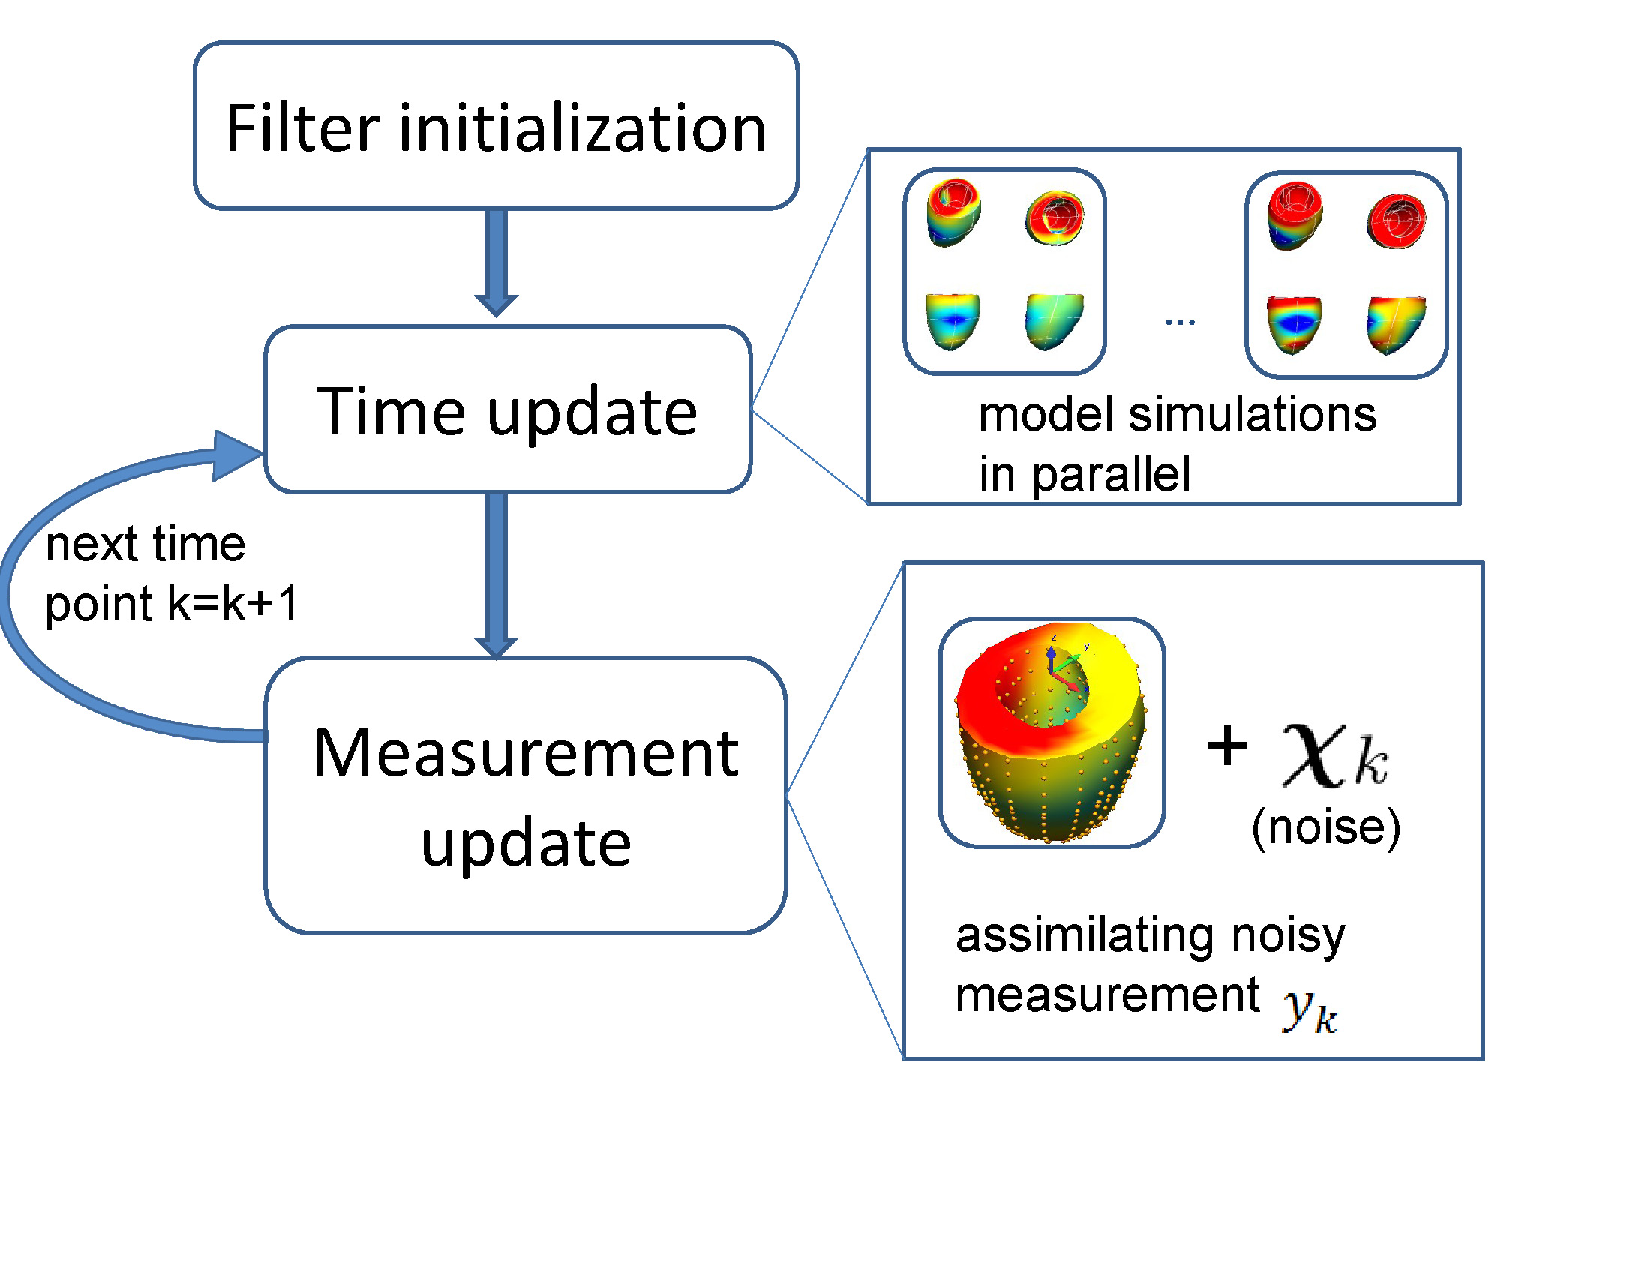
\includegraphics[width=110mm]{ParameterEstimation/2010-08-09-rUKF-estimation-workflow.pdf} %Width: 2001 pixels  Height: 1501 pixels
\caption{Schematic illustration of the estimation procedure via rUKF.}
\label{fig:schmeatic-rUKF}
\end{figure}


\subsubsection{Parameter estimator equations}
\label{sec-parameter-estimation-eq}
Our objective is to estimate constitutive parameters (table \ref{tab-cuccioneLawParameters}) in the mechanical system (eq. \ref{quasistatic_system_equation} and \ref{eq-measurement}) formulated in previous section. This is achieved by applying filtering on estimating the augmented state vector $\vect{z}_k$ (equation \ref{eq-augmented-state}).

%For the filtering on , we adopt rUKF  with canonical unscented transformation to improve estimation accuracy and to avoid possible numerical instability.
%In unscented Kalman filter (UKF), the statistics of a random variable that undergoes a nonlinear transformation is calculated through unscented transformation or sampling at \emph{sigma points}. It is the preferable choice for assimilating measurements into nonlinear systems since it has superior performance than the traditionally used extended Kalman filter (\citealt{Julier1995New}, \citealt[p. 441]{Simon2006Optimal}).

Compared with widely-employed unscented Kalman filter (UKF, \citealt{Julier1995New}), reduced-order UKF (rUKF, \citealt{Moireau2010Reduced}) essentially reduces the rank of the error covariance matrix of the augmented state vector $\vect{z}_k$ from full rank $n_\textnormal{z}$ to $r$, where
\begin{align}
r &\ll n_\textnormal{z}, \quad \vect{z}_k \in \Real^{n_\textnormal{z}}  \textnormal{ (i.e., $n_\textnormal{z}$ is the size of augmented state vector $\vect{z}_k$)}, \label{eq-system-size-01}
\end{align}
and
\begin{align}
r &\ll m, \quad \vect{y}_k \in \Real^{m} \textnormal{ (i.e., $m$ is the size of measurement vector $\vect{y}_k$)}. \label{eq-system-size-02}
\end{align}
With this simplification, the covariance matrix storage is reduced from $n_\textnormal{z} \times n_\textnormal{z}$ to $n_\textnormal{z} \times r$ and the matrix inversion operation can be performed in a subspace $\Matrix^{r \times r}$ instead of $\Matrix^{m \times m}$. Furthermore, the number of model evaluations required by the filter at each time point is also significant decreased, roughly from $O(n_\textnormal{z})$ to $O(r)$. As mentioned in remark (\ref{se-remark-quasitatic}), in the quasi-static systems the uncertainties primarily lie in the parameter space, and thus $r$ can be chosen as the dimension of parameter space, that is
\begin{align}
    r=n_\theta, \quad \vect{\theta}_k \in \Real^{n_\theta} \textnormal{ (i.e., $n_\theta$ is the size of parameter vector $\vect{\theta}_k$)}. \label{eq-system-size-03}
\end{align}


The filtering process consists of three steps (figure \ref{fig:schmeatic-rUKF}) -- initialization of the augmented state vector $\hat{\vect{z}}_{0}^{+}$ and its error matrix $\matr{P}_0^+$, their time updates involving one-step model evaluations, and measurement updates where the noisy data are assimilated based on the relative confidence of the model prediction and measurements accuracy.   In the following notations, we use superscripts $-$ and $+$ to differentiate the prior and posterior estimations (variables before and after assimilating measurements), and $\, \hat{ } \, $  for indicating estimated variables (the mean of the true variable value). Subscript $k$ is the time points with $0$ as the initialization time point.

\subsubsection*{Filter initialization}
For filter initialization, the initial error-covariance $\matr{P}_0^+  \in \Matrix^{n_\textnormal{z} \times n_\textnormal{z}}$, which is typically prescribed as a diagonal matrix with $r$ non-zero elements representing the uncertainties of the system parameters, is decomposed using singular value decomposition (SVD) method
\begin{align}
\matr{P}_0^+ &= \matr{L}_0^+ \matr{\Lambda}_0^+ {\matr{L}_0^+}^T , \label{eq-SEUK-initialization-01}
\end{align}
where $\matr{L}_0^+ \in \Matrix^{n_\textnormal{z} \times n_\textnormal{z}}$ and $\matr{\Lambda}_0^+ \in \Matrix^{n_\textnormal{z} \times n_\textnormal{z}}$ are orthonormal and diagonal matrices respectively.

We keep the first $r$ eigenvectors $\matr{L}_0^+(: \, ,1:r)$ (here this notation denotes the sub-matrix consisting of all the rows and $1$ to $r$ columns of $\matr{L}_0^+$) of $\matr{P}_0^+$, and define its reduced-rank square-root approximation $\matr{S}_0^+ \in \Matrix^{n_\textnormal{z} \times r}$ as
\begin{align}
\matr{S}_0^+ &= \matr{L}_0(: \, ,1:r)\sqrt{\matr{\Lambda}_0^+(1:r,1:r)}. \label{eq-SEUK-initialization-02}
\end{align}
The $r$ column vectors of $\matr{S}$ span the space in which the filter is allowed to make corrections to the augmented state vector $\vect{z}$.

\subsubsection*{Time update}
In time update phase, $2r$ model simulations $f(\hat{\vect{z}}_{k-1}^{+(i)},\vect{u}_{k-1})$ (recall equation \ref{quasistatic_system_equation}) are performed at a set of sampling points $\hat{\vect{z}}_{k-1}^{+(i)}$, in parallel:
\begin{align}
\hat{\vect{z}}_k^{-(i)} &= f(\hat{\vect{z}}_{k-1}^{+(i)},\vect{u}_{k-1}).
\end{align}

These sampling points are referred to as \emph{sigma points} if they are constructed by the so-called \emph{unscented transformation} (\citealt{Julier1997New}). Sigma points are deliberately constructed so that they have the same known statics, e.g., first and second and possibly higher moments, as the given estimate.

While a minimal set of $r+1$ sigma points are adequate to preserve the first and second moments (mean and covariance), we have adopted a \emph{symmetric} set of $2r$-sigma points to improve estimation accuracy, based on the assumption that error processes associated with calibrated measuring devices exhibit the symmetries about a set of principle measurement axes, and such symmetries provide information about the third central moment of the unknown distribution of estimated variables (\citealt{Julier2002Reduced}). We generate the $2r$ sigma points $\hat{\vect{z}}_{k-1}^{+(i)}$ from the reduced-rank square-root approximation matrix $\matr{S}$ by
\begin{align}
\hat{\vect{z}}_{k-1}^{+(i)} &= \hat{\vect{z}}_{k-1}^{+} + \tilde{\vect{z}}_{k-1}^{+(i)},\quad i=1,...,2r, \label{eq-unscented-transformation-01}
\end{align}
where
\begin{align}
\tilde{\vect{z}}_{k-1}^{+(i)}&=\matr{S}^{-}_{k-1}(:,i),\quad i=1,...,r,\label{eq-unscented-transformation-02}
\end{align}
and
\begin{align}
\tilde{\vect{z}}_{k-1}^{+(i)}&=-\matr{S}^{-}_{k-1}(:,i-r),\quad i=r+1,...,2r. \label{eq-unscented-transformation-03}
\end{align}

The statistics (mean $\hat{\vect{z}}_k^{-}$ and error covariance $\matr{P}_k^-$) of the augmented state variable $\vect{z}_k^{-}$ are estimated from the transformed sampling set by
\begin{align}
\hat{\vect{z}}_k^{-} &= \frac{1}{2r} \sum_{i=1}^{2r} \hat{\vect{z}}_k^{-(i)},\\
\matr{P}_k^- &= \frac{1}{\sqrt{2 \rho r}}  \sum_{i=1}^{2r} (\hat{\vect{z}}_k^{-(i)}-\hat{\vect{z}}_k^{-}) (\hat{\vect{z}}_k^{-(i)}-\hat{\vect{z}}_k^{-})^T, \label{eq-analysis-error-covariance}
\end{align}
where $\rho$ (typically $\rho \in [0.9,1]$) is an additional ``fading" parameter to prevent filter divergence through artificially increase the error covariance matrix (\citealt{Brasseur2006SEEK}).

To keep the rank of $\matr{P}_k^-$ to be $r$, we again decompose $\matr{P}_k^-$ as eq. (\ref{eq-SEUK-initialization-01}) and (\ref{eq-SEUK-initialization-02}) to reobtain the  reduced-rank square-root approximation $\matr{S}_{k}^-$ of $\matr{P}_k^-$:
\begin{align}
\opSVD(\matr{P}_k^-) &\to  \matr{S}_{k}^- (\matr{S}_{k}^-)^T.
\end{align}
We point out that the SVD operation in above equation can be computed efficiently without assembling the full $P_k^-$ (\citealt{Moireau2010Reduced}).

\subsubsection*{Measurement update}
Recalling equation (\ref{eq-measurement03}), the observation operator can be adequately written as the observational matrix $\matr{H}$ for our problem. In the measurement update phase, the observation $\vect{y}_k$ is assimilated into the prior estimation $\hat{\vect{z}}_k^-$ to give the posterior estimation based on the \emph{innovation or Kalman gain matrix} $\matr{K}_k$ by
\begin{align}
\hat{\vect{z}}_k^+ &= \hat{\vect{z}}_k^- + \matr{K}_k(\vect{y}_k - \matr{H} \hat{\vect{z}}_k^{-}),
\end{align}
In the above equation, the Kalman gain matrix $\matr{K}_k$ in rUKF can be obtained by applying the matrix inverse lemma (see e.g., \citealt{Simon2006Optimal}) to that for the UKF
\begin{align}
\matr{K}_k &=  \matr{S}_{k}^- (\matr{I} + (\matr{H} \matr{S}_{k}^-)^T \matr{R}_\textnormal{d}^{-1} \matr{H} \matr{S}_{k}^-)^{-1} (\matr{H} \matr{S}_{k}^-)^T \matr{R}_\textnormal{d}^{-1},
\end{align}
where $\matr{R}_\textnormal{d}$ is the measurement error covariance matrix (recall equation \ref{eq-measurement02}). The square-root approximation of error covariance $\matr{S}_{k}$ is updated as
\begin{align}
\matr{S}_{k}^+ &= \matr{S}_{k}^- (\matr{I} + (\matr{H} \matr{S}_{k}^-)^T \matr{R}_\textnormal{d}^{-1} \matr{H} \matr{S}_{k}^-)^{-1/2}.
\end{align}
Note that the matrix inverse and square-root operations in the above equations are performed on $\matr{I} + (\matr{H} \matr{S}_{k}^-)^T \matr{R}_\textnormal{d}^{-1} \matr{H} \matr{S}_{k}^-$ (as mentioned before at the beginning of this section), which reduces the computational cost significantly for large systems.

For further details and formal derivations of the equations in rUKF, please refer to \citet{Moireau2010Reduced}, in particular when the observation operator is nonlinear, which makes the expression of the filter much more intricate. As a summary, rUKF decreases the computational costs dramatically based on the assumption that the rank of error covariance (second order moment) can be reduced. However, filter optimality might be lost because of this simplification, and thus the performance of this filter on our cubic-Hermite interpolation based mechanical model needs to be assessed numerically (see results in the next section), especially with the introduction of measurement noise and exponential-form constitutive law.
                         %input from ParameterEstimation/ParameterEstimation.tex

\clearemptydoublepage
\addcontentsline{toc}{chapter}{\numberline{}References}

\renewcommand{\bibname}{References}

%\bibliographystyle{agsm}
\bibliographystyle{alpha}
\bibliography{../references/references,ParameterEstimation/ParameterEstimationReference} 
%bibliography from ../references/references.bib and ParameterEstimation/ParameterEstimationReference.bib

%%% Local Variables: 
%%% mode: latex
%%% TeX-master: 
%%% End: 
               %input from References/References.tex

\clearemptydoublepage
\addcontentsline{toc}{chapter}{\numberline{}Index}

\printindex

%%% Local Variables: 
%%% mode: latex
%%% TeX-master: 
%%% End: 
                         %input from Index/Index.tex

\end{document}   

%%% Local Variables: 
%%% mode: latex
%%% TeX-master: t
%%% End: 
